\section{Sparsity Patterns}

In this section, a number of sparsity patterns (a visualization of the potential nonzero entries in a matrix) are shown for the \qp{} matrices (see Fig.~\ref{fig:overview}).
The symbol \scalebox{1.5}{\mysparsesymbol} indicates a potential nonzero entry in the matrix and \scalebox{1.5}{\mytemp} indices a potential nonzero entry if we only look at the specific term mentioned.
In all the figures, $\{n_u, n_\xi, n_p, N_t \}$ are $\{1, 2, 2, 7\}$.

\begin{figure}[ht]

\centering

\begin{subfigure}{0.33\textwidth}
\centering
\begin{minipage}{1\textwidth}
\tikzsetnextfilename{Huu}

\centering
\resizebox{1\textwidth}{!}{
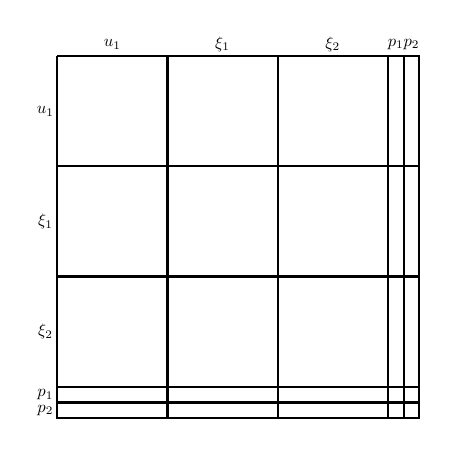
\begin{tikzpicture}[yscale=-1] 

\pgfmathsetmacro{\nt}{7};% time points
\pgfmathsetmacro{\nu}{1}; % controls
\pgfmathsetmacro{\nx}{2}; % states
\pgfmathsetmacro{\np}{2}; % parameters
\pgfmathsetmacro{\nc}{\nu + \nx}; % total continuous

%% control labels
\foreach \k in {1,...,\nu}{
	\pgfmathsetmacro{\x}{0.2*\nt*\k - 0.2/2*(\nt-1)};
	\node () at (\x,-0.05) {\scalebox{0.6}{$u_{\k}$}};
    \node () at (-0.05,\x) {\scalebox{0.6}{$u_{\k}$}};
}

%% state labels
\foreach \k in {1,...,\nx}{
	\pgfmathsetmacro{\x}{0.2*\nt*\k + 0.2*\nu*\nt - 0.2/2*(\nt-1)};
	\node () at (\x,-0.05) {\scalebox{0.6}{$\xi_{\k}$}};
    \node () at (-0.05,\x) {\scalebox{0.6}{$\xi_{\k}$}};
}

%% parameter labels
\foreach \k in {1,...,\np}{
	\pgfmathsetmacro{\x}{0.2*\k + 0.2*\nu*\nt + 0.2*\nx*\nt};
	\node () at (\x,-0.05) {\scalebox{0.6}{$p_{\k}$}};
    \node () at (-0.05,\x) {\scalebox{0.6}{$p_{\k}$}};
}


%% controls
\foreach \k in {1,...,\nu}{
	\foreach \j in {1,...,\nu}{
		\foreach \i in {1,...,\nt}{ 
        	\pgfmathsetmacro{\kk}{\k-1};
            \pgfmathsetmacro{\jj}{\j-1};
        	\pgfmathsetmacro{\x}{0.2*\i + 0.2*\kk*\nt};
            \pgfmathsetmacro{\y}{0.2*\i + 0.2*\jj*\nt};
        	\node () at (\x,\y) {\mysparsesymbol};
} 
    \pgfmathsetmacro{\kk}{\k-1};
    \pgfmathsetmacro{\jj}{\j-1};
    \pgfmathsetmacro{\x}{0.2*\kk*\nt + 0.1};
    \pgfmathsetmacro{\y}{0.2*\jj*\nt + 0.1};
	\draw[\mysparseboxcolor,thick](\x,\y) -- (\x+0.2*\nt,\y) -- (\x+0.2*\nt,\y+0.2*\nt) -- (\x,\y+0.2*\nt) -- (\x,\y);
} }

%% states
\foreach \k in {1,...,\nx}{
	\foreach \j in {1,...,\nx}{
		\foreach \i in {1,...,\nt}{ 
        	\pgfmathsetmacro{\kk}{\k-1};
            \pgfmathsetmacro{\jj}{\j-1};
        	\node () at (0.2*\i + 0.2*\kk*\nt + 0.2*\nu*\nt, 0.2*\i + 0.2*\jj*\nt + 0.2*\nu*\nt) {\mysparsesymbol};
} 
    \pgfmathsetmacro{\kk}{\k-1};
    \pgfmathsetmacro{\jj}{\j-1};
    \pgfmathsetmacro{\x}{0.2*\kk*\nt + 0.2*(\nu)*\nt + 0.1};
    \pgfmathsetmacro{\y}{0.2*\jj*\nt + 0.2*(\nu)*\nt + 0.1};
	\draw[\mysparseboxcolor,thick](\x,\y) -- (\x+0.2*\nt,\y) -- (\x+0.2*\nt,\y+0.2*\nt) -- (\x,\y+0.2*\nt) -- (\x,\y);
} }

%% parameters
\foreach \k in {1,...,\np}{
	\foreach \j in {1,...,\np}{
      \pgfmathsetmacro{\kk}{\k-1};
      \pgfmathsetmacro{\jj}{\j-1};
      \node ( ) at (0.2*\j + 0.2*\nx*\nt + 0.2*\nu*\nt, 0.2*\k + 0.2*\nx*\nt + 0.2*\nu*\nt) {\mysparsesymbol};
      \pgfmathsetmacro{\x}{0.2*\kk + 0.2*(\nu)*\nt + 0.2*\nx*\nt + 0.1};
      \pgfmathsetmacro{\y}{0.2*\jj + 0.2*(\nu)*\nt + 0.2*\nx*\nt + 0.1};
      \draw[\mysparseboxcolor,thick](\x,\y) -- (\x+0.2,\y) -- (\x+0.2,\y+0.2) -- (\x,\y+0.2) -- (\x,\y);
} }

%% states and controls
\foreach \k in {1,...,\nu}{
	\foreach \j in {1,...,\nx}{
		\foreach \i in {1,...,\nt}{ 
        	\pgfmathsetmacro{\kk}{\k-1};
            \pgfmathsetmacro{\jj}{\j-1};
        	\node () at ( 0.2*\i + 0.2*\kk*\nt , 0.2*\i + 0.2*\jj*\nt + 0.2*\nu*\nt) {\mysparsesymbol};
        	\node () at ( 0.2*\i + 0.2*\jj*\nt + 0.2*\nu*\nt, 0.2*\i + 0.2*\kk*\nt) {\mysparsesymbol};
} 
    \pgfmathsetmacro{\kk}{\k-1};
    \pgfmathsetmacro{\jj}{\j-1};
    \pgfmathsetmacro{\x}{0.2*\kk*\nt + 0.1};
    \pgfmathsetmacro{\y}{0.2*\jj*\nt + 0.2*(\nu)*\nt + 0.1};
	\draw[\mysparseboxcolor,thick](\x,\y) -- (\x+0.2*\nt,\y) -- (\x+0.2*\nt,\y+0.2*\nt) -- (\x,\y+0.2*\nt) -- (\x,\y);
    \draw[\mysparseboxcolor,thick](\y,\x) -- (\y+0.2*\nt,\x) -- (\y+0.2*\nt,\x+0.2*\nt) -- (\y,\x+0.2*\nt) -- (\y,\x);
} }

%% states and parameters
\foreach \k in {1,...,\np}{
	\foreach \j in {1,...,\nx}{
		\foreach \i in {1,...,\nt}{ 
        	\pgfmathsetmacro{\kk}{\k-1};
            \pgfmathsetmacro{\jj}{\j-1};
        	\node () at ( 0.2*\k + 0.2*\nx*\nt + 0.2*\nu*\nt, 0.2*\i + 0.2*\jj*\nt + 0.2*\nu*\nt ) {\mysparsesymbol};
            \node () at ( 0.2*\i + 0.2*\jj*\nt + 0.2*\nu*\nt, 0.2*\k + 0.2*\nx*\nt + 0.2*\nu*\nt ) {\mysparsesymbol};
} 
    \pgfmathsetmacro{\kk}{\k-1};
    \pgfmathsetmacro{\jj}{\j-1};
    \pgfmathsetmacro{\x}{0.2*\kk + 0.2*\nx*\nt + 0.2*\nu*\nt + 0.1};
    \pgfmathsetmacro{\y}{0.2*\jj*\nt + 0.2*\nu*\nt + 0.1};
	\draw[\mysparseboxcolor,thick](\x,\y) -- (\x+0.2,\y) -- (\x+0.2,\y+0.2*\nt) -- (\x,\y+0.2*\nt) -- (\x,\y);
    \draw[\mysparseboxcolor,thick](\y,\x) -- (\y+0.2*\nt,\x) -- (\y+0.2*\nt,\x+0.2) -- (\y,\x+0.2) -- (\y,\x);

} }

%% controls and parameters
\foreach \k in {1,...,\np}{
	\foreach \j in {1,...,\nu}{
		\foreach \i in {1,...,\nt}{ 
        	\pgfmathsetmacro{\kk}{\k-1};
            \pgfmathsetmacro{\jj}{\j-1};
        	\node () at ( 0.2*\k + 0.2*\nx*\nt + 0.2*\nu*\nt, 0.2*\i + 0.2*\jj*\nt ) {\mysparsesymbol};
            \node () at ( 0.2*\i + 0.2*\jj*\nt , 0.2*\k + 0.2*\nx*\nt + 0.2*\nu*\nt ) {\mysparsesymbol};
} 
    \pgfmathsetmacro{\kk}{\k-1};
    \pgfmathsetmacro{\jj}{\j-1};
    \pgfmathsetmacro{\x}{0.2*\kk + 0.2*\nx*\nt + 0.2*\nu*\nt + 0.1};
    \pgfmathsetmacro{\y}{0.2*\jj*\nt + 0.1};
	\draw[\mysparseboxcolor,thick](\x,\y) -- (\x+0.2,\y) -- (\x+0.2,\y+0.2*\nt) -- (\x,\y+0.2*\nt) -- (\x,\y);
    \draw[\mysparseboxcolor,thick](\y,\x) -- (\y+0.2*\nt,\x) -- (\y+0.2*\nt,\x+0.2) -- (\y,\x+0.2) -- (\y,\x);
} }

%% initial states
\foreach \k in {1,...,\nx}{
	\foreach \j in {1,...,\nc}{
		\foreach \i in {1,...,\nt}{ 
        	\pgfmathsetmacro{\kk}{\k-1};
            \pgfmathsetmacro{\jj}{\j-1};
        	\node () at (0.2 + 0.2*\kk*\nt + 0.2*\nu*\nt, 0.2*\i + 0.2*\jj*\nt ) {\mysparsesymbol};
            \node () at ( 0.2*\i + 0.2*\jj*\nt , 0.2 + 0.2*\kk*\nt + 0.2*\nu*\nt ) {\mysparsesymbol};
} } 
	\foreach \j in {1,...,\np}{
		\pgfmathsetmacro{\kk}{\k-1};
        \pgfmathsetmacro{\jj}{\j-1};
        \node () at ( 0.2*\k + 0.2*\nx*\nt + 0.2*\nu*\nt, 0.2 + 0.2*\jj*\nt + 0.2*\nu*\nt ) {\mysparsesymbol};
        \node () at ( 0.2 + 0.2*\jj*\nt + 0.2*\nu*\nt , 0.2*\k + 0.2*\nx*\nt + 0.2*\nu*\nt ) {\mysparsesymbol};
	}
}

%% final states
\foreach \k in {1,...,\nx}{
	\foreach \j in {1,...,\nc}{
		\foreach \i in {1,...,\nt}{ 
        	\pgfmathsetmacro{\kk}{\k-1};
            \pgfmathsetmacro{\jj}{\j-1};
        	\node () at (0.2*\nt + 0.2*\kk*\nt + 0.2*\nu*\nt, 0.2*\i + 0.2*\jj*\nt ) {\mysparsesymbol};
            \node () at ( 0.2*\i + 0.2*\jj*\nt , 0.2*\nt + 0.2*\kk*\nt + 0.2*\nu*\nt ) {\mysparsesymbol};
} } 
	\foreach \j in {1,...,\np}{
		\pgfmathsetmacro{\kk}{\k-1};
        \pgfmathsetmacro{\jj}{\j-1};
        \node () at ( 0.2*\k + 0.2*\nx*\nt + 0.2*\nu*\nt, 0.2*\nt + 0.2*\jj*\nt + 0.2*\nu*\nt ) {\mysparsesymbol};
        \node () at ( 0.2*\nt + 0.2*\jj*\nt + 0.2*\nu*\nt , 0.2*\k + 0.2*\nx*\nt + 0.2*\nu*\nt ) {\mysparsesymbol};
	}
}


























% %% states and controls
% \foreach \k in {0,...,2}{
% 	\foreach \j in {0,...,2}{
% 		\foreach \i in {1,...,5}{ 
%         	\node () at (0.2*\i + \k,0.2*\i + \j) {\mysparsesymbol};
% } } }

% %% parameters - right
% \foreach \k in {0,...,1}{
% 	\foreach \j in {0,...,2}{
% 		\foreach \i in {1,...,5}{
%         	\node ( ) at (0.2*\k + 3.2, 0.2*\i + \j) {\mysparsesymbol};
% } } }

% %% parameters - bottom
% \foreach \k in {0,...,1}{
% 	\foreach \j in {0,...,2}{
% 		\foreach \i in {1,...,5}{
%         	\node ( ) at (0.2*\i + \j, 0.2*\k + 3.2) {\mysparsesymbol};
% } } }

% %% parameters - corner
% \foreach \k in {0,...,1}{
% 	\foreach \j in {0,...,1}{
%         	\node ( ) at (0.2*\j + 3.2, 0.2*\k + 3.2) {\mysparsesymbol};
% } }

% %% initial states - bottom
% \foreach \k in {0,...,1}{
% 	\foreach \j in {0,...,2}{
% 		\foreach \i in {1,...,5}{
%         	\node ( ) at (0.2*\i + \j, \k + 1.2) {\mysparsesymbol};
% } } }

% %% final states - bottom
% \foreach \k in {0,...,1}{
% 	\foreach \j in {0,...,2}{
% 		\foreach \i in {1,...,5}{
%         	\node ( ) at (0.2*\i + \j, \k + 2.0) {\mysparsesymbol};
% } } }

% %% initial states - right
% \foreach \k in {0,...,1}{
% 	\foreach \j in {0,...,2}{
% 		\foreach \i in {1,...,5}{
%         	\node ( ) at (\k + 1.2, 0.2*\i + \j) {\mysparsesymbol};
% } } }

% %% final states - right
% \foreach \k in {0,...,1}{
% 	\foreach \j in {0,...,2}{
% 		\foreach \i in {1,...,5}{
%         	\node ( ) at (\k + 2.0, 0.2*\i + \j) {\mysparsesymbol};
% } } }


% %% draw boxes - states and controls
% \foreach \k in {0,...,2}{
% 	\foreach \j in {0,...,2}{
%     	\pgfmathsetmacro{\x}{\k + 0.1};
%     	\pgfmathsetmacro{\y}{\j + 0.1};
%         \draw[blue!70] (\x,\y) -- (\x+1,\y) -- (\x+1,\y+1) -- (\x,\y+1) -- (\x,\y);
% } }

% %% draw boxes - parameters - right
% \foreach \k in {0,...,1}{
% 	\foreach \j in {0,...,2}{
%     	\pgfmathsetmacro{\x}{0.2*\k + 0.1 + 3};
%     	\pgfmathsetmacro{\y}{\j + 0.1};
%         \draw[blue] (\x,\y) -- (\x+0.2,\y) -- (\x+0.2,\y+1) -- (\x,\y+1) -- (\x,\y);
% } }

% %% draw boxes - parameters - bottom
% \foreach \k in {0,...,2}{
% 	\foreach \j in {0,...,1}{
%     	\pgfmathsetmacro{\x}{\k + 0.1};
%     	\pgfmathsetmacro{\y}{0.2*\j + 0.1 + 3};
%         \draw[blue] (\x,\y) -- (\x+1,\y) -- (\x+1,\y+0.2) -- (\x,\y+0.2) -- (\x,\y);
% } }

% %% draw boxes - parameters - bottom
% \foreach \k in {0,...,1}{
% 	\foreach \j in {0,...,1}{
%     	\pgfmathsetmacro{\x}{0.2*\k + 0.1 + 3};
%     	\pgfmathsetmacro{\y}{0.2*\j + 0.1 + 3};
%         \draw[blue] (\x,\y) -- (\x+0.2,\y) -- (\x+0.2,\y+0.2) -- (\x,\y+0.2) -- (\x,\y);
% } }


%% controls
\foreach \k in {1,...,\nu}{
	\foreach \j in {1,...,\nu}{
		\foreach \i in {1,...,\nt}{ 
        	\pgfmathsetmacro{\kk}{\k-1};
            \pgfmathsetmacro{\jj}{\j-1};
        	\pgfmathsetmacro{\x}{0.2*\i + 0.2*\kk*\nt};
            \pgfmathsetmacro{\y}{0.2*\i + 0.2*\jj*\nt};
        	\node () at (\x,\y) {\mytemp};
} } }
\end{tikzpicture}
}
\end{minipage}
\caption{$\bm{L}_{11}$ terms.}
\label{fig:L11}
\end{subfigure}%
\begin{subfigure}{0.33\textwidth}
\centering
\begin{minipage}{1\textwidth}
\input{../ch5/sparsity/Hxx}
\end{minipage}
\caption{$\bm{L}_{22}$ terms.}
\label{fig:L22}
\end{subfigure}%
\begin{subfigure}{0.33\textwidth}
\centering
\begin{minipage}{1\textwidth}
\tikzsetnextfilename{Hpp}

\centering
\resizebox{1\textwidth}{!}{
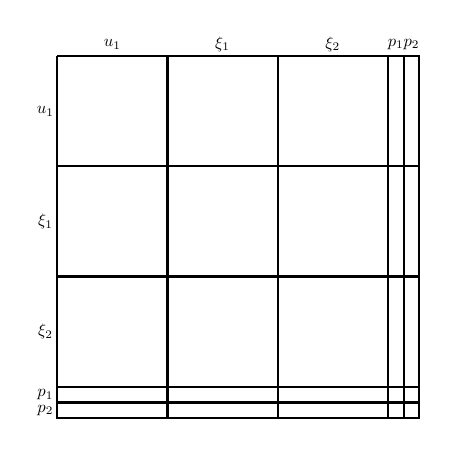
\begin{tikzpicture}[yscale=-1] 

\pgfmathsetmacro{\nt}{7};% time points
\pgfmathsetmacro{\nu}{1}; % controls
\pgfmathsetmacro{\nx}{2}; % states
\pgfmathsetmacro{\np}{2}; % parameters
\pgfmathsetmacro{\nc}{\nu + \nx}; % total continuous

%% control labels
\foreach \k in {1,...,\nu}{
	\pgfmathsetmacro{\x}{0.2*\nt*\k - 0.2/2*(\nt-1)};
	\node () at (\x,-0.05) {\scalebox{0.6}{$u_{\k}$}};
    \node () at (-0.05,\x) {\scalebox{0.6}{$u_{\k}$}};
}

%% state labels
\foreach \k in {1,...,\nx}{
	\pgfmathsetmacro{\x}{0.2*\nt*\k + 0.2*\nu*\nt - 0.2/2*(\nt-1)};
	\node () at (\x,-0.05) {\scalebox{0.6}{$\xi_{\k}$}};
    \node () at (-0.05,\x) {\scalebox{0.6}{$\xi_{\k}$}};
}

%% parameter labels
\foreach \k in {1,...,\np}{
	\pgfmathsetmacro{\x}{0.2*\k + 0.2*\nu*\nt + 0.2*\nx*\nt};
	\node () at (\x,-0.05) {\scalebox{0.6}{$p_{\k}$}};
    \node () at (-0.05,\x) {\scalebox{0.6}{$p_{\k}$}};
}


%% controls
\foreach \k in {1,...,\nu}{
	\foreach \j in {1,...,\nu}{
		\foreach \i in {1,...,\nt}{ 
        	\pgfmathsetmacro{\kk}{\k-1};
            \pgfmathsetmacro{\jj}{\j-1};
        	\pgfmathsetmacro{\x}{0.2*\i + 0.2*\kk*\nt};
            \pgfmathsetmacro{\y}{0.2*\i + 0.2*\jj*\nt};
        	\node () at (\x,\y) {\mysparsesymbol};
} 
    \pgfmathsetmacro{\kk}{\k-1};
    \pgfmathsetmacro{\jj}{\j-1};
    \pgfmathsetmacro{\x}{0.2*\kk*\nt + 0.1};
    \pgfmathsetmacro{\y}{0.2*\jj*\nt + 0.1};
	\draw[\mysparseboxcolor,thick](\x,\y) -- (\x+0.2*\nt,\y) -- (\x+0.2*\nt,\y+0.2*\nt) -- (\x,\y+0.2*\nt) -- (\x,\y);
} }

%% states
\foreach \k in {1,...,\nx}{
	\foreach \j in {1,...,\nx}{
		\foreach \i in {1,...,\nt}{ 
        	\pgfmathsetmacro{\kk}{\k-1};
            \pgfmathsetmacro{\jj}{\j-1};
        	\node () at (0.2*\i + 0.2*\kk*\nt + 0.2*\nu*\nt, 0.2*\i + 0.2*\jj*\nt + 0.2*\nu*\nt) {\mysparsesymbol};
} 
    \pgfmathsetmacro{\kk}{\k-1};
    \pgfmathsetmacro{\jj}{\j-1};
    \pgfmathsetmacro{\x}{0.2*\kk*\nt + 0.2*(\nu)*\nt + 0.1};
    \pgfmathsetmacro{\y}{0.2*\jj*\nt + 0.2*(\nu)*\nt + 0.1};
	\draw[\mysparseboxcolor,thick](\x,\y) -- (\x+0.2*\nt,\y) -- (\x+0.2*\nt,\y+0.2*\nt) -- (\x,\y+0.2*\nt) -- (\x,\y);
} }

%% parameters
\foreach \k in {1,...,\np}{
	\foreach \j in {1,...,\np}{
      \pgfmathsetmacro{\kk}{\k-1};
      \pgfmathsetmacro{\jj}{\j-1};
      \node ( ) at (0.2*\j + 0.2*\nx*\nt + 0.2*\nu*\nt, 0.2*\k + 0.2*\nx*\nt + 0.2*\nu*\nt) {\mysparsesymbol};
      \pgfmathsetmacro{\x}{0.2*\kk + 0.2*(\nu)*\nt + 0.2*\nx*\nt + 0.1};
      \pgfmathsetmacro{\y}{0.2*\jj + 0.2*(\nu)*\nt + 0.2*\nx*\nt + 0.1};
      \draw[\mysparseboxcolor,thick](\x,\y) -- (\x+0.2,\y) -- (\x+0.2,\y+0.2) -- (\x,\y+0.2) -- (\x,\y);
} }

%% states and controls
\foreach \k in {1,...,\nu}{
	\foreach \j in {1,...,\nx}{
		\foreach \i in {1,...,\nt}{ 
        	\pgfmathsetmacro{\kk}{\k-1};
            \pgfmathsetmacro{\jj}{\j-1};
        	\node () at ( 0.2*\i + 0.2*\kk*\nt , 0.2*\i + 0.2*\jj*\nt + 0.2*\nu*\nt) {\mysparsesymbol};
        	\node () at ( 0.2*\i + 0.2*\jj*\nt + 0.2*\nu*\nt, 0.2*\i + 0.2*\kk*\nt) {\mysparsesymbol};
} 
    \pgfmathsetmacro{\kk}{\k-1};
    \pgfmathsetmacro{\jj}{\j-1};
    \pgfmathsetmacro{\x}{0.2*\kk*\nt + 0.1};
    \pgfmathsetmacro{\y}{0.2*\jj*\nt + 0.2*(\nu)*\nt + 0.1};
	\draw[\mysparseboxcolor,thick](\x,\y) -- (\x+0.2*\nt,\y) -- (\x+0.2*\nt,\y+0.2*\nt) -- (\x,\y+0.2*\nt) -- (\x,\y);
    \draw[\mysparseboxcolor,thick](\y,\x) -- (\y+0.2*\nt,\x) -- (\y+0.2*\nt,\x+0.2*\nt) -- (\y,\x+0.2*\nt) -- (\y,\x);
} }

%% states and parameters
\foreach \k in {1,...,\np}{
	\foreach \j in {1,...,\nx}{
		\foreach \i in {1,...,\nt}{ 
        	\pgfmathsetmacro{\kk}{\k-1};
            \pgfmathsetmacro{\jj}{\j-1};
        	\node () at ( 0.2*\k + 0.2*\nx*\nt + 0.2*\nu*\nt, 0.2*\i + 0.2*\jj*\nt + 0.2*\nu*\nt ) {\mysparsesymbol};
            \node () at ( 0.2*\i + 0.2*\jj*\nt + 0.2*\nu*\nt, 0.2*\k + 0.2*\nx*\nt + 0.2*\nu*\nt ) {\mysparsesymbol};
} 
    \pgfmathsetmacro{\kk}{\k-1};
    \pgfmathsetmacro{\jj}{\j-1};
    \pgfmathsetmacro{\x}{0.2*\kk + 0.2*\nx*\nt + 0.2*\nu*\nt + 0.1};
    \pgfmathsetmacro{\y}{0.2*\jj*\nt + 0.2*\nu*\nt + 0.1};
	\draw[\mysparseboxcolor,thick](\x,\y) -- (\x+0.2,\y) -- (\x+0.2,\y+0.2*\nt) -- (\x,\y+0.2*\nt) -- (\x,\y);
    \draw[\mysparseboxcolor,thick](\y,\x) -- (\y+0.2*\nt,\x) -- (\y+0.2*\nt,\x+0.2) -- (\y,\x+0.2) -- (\y,\x);

} }

%% controls and parameters
\foreach \k in {1,...,\np}{
	\foreach \j in {1,...,\nu}{
		\foreach \i in {1,...,\nt}{ 
        	\pgfmathsetmacro{\kk}{\k-1};
            \pgfmathsetmacro{\jj}{\j-1};
        	\node () at ( 0.2*\k + 0.2*\nx*\nt + 0.2*\nu*\nt, 0.2*\i + 0.2*\jj*\nt ) {\mysparsesymbol};
            \node () at ( 0.2*\i + 0.2*\jj*\nt , 0.2*\k + 0.2*\nx*\nt + 0.2*\nu*\nt ) {\mysparsesymbol};
} 
    \pgfmathsetmacro{\kk}{\k-1};
    \pgfmathsetmacro{\jj}{\j-1};
    \pgfmathsetmacro{\x}{0.2*\kk + 0.2*\nx*\nt + 0.2*\nu*\nt + 0.1};
    \pgfmathsetmacro{\y}{0.2*\jj*\nt + 0.1};
	\draw[\mysparseboxcolor,thick](\x,\y) -- (\x+0.2,\y) -- (\x+0.2,\y+0.2*\nt) -- (\x,\y+0.2*\nt) -- (\x,\y);
    \draw[\mysparseboxcolor,thick](\y,\x) -- (\y+0.2*\nt,\x) -- (\y+0.2*\nt,\x+0.2) -- (\y,\x+0.2) -- (\y,\x);
} }

%% initial states
\foreach \k in {1,...,\nx}{
	\foreach \j in {1,...,\nc}{
		\foreach \i in {1,...,\nt}{ 
        	\pgfmathsetmacro{\kk}{\k-1};
            \pgfmathsetmacro{\jj}{\j-1};
        	\node () at (0.2 + 0.2*\kk*\nt + 0.2*\nu*\nt, 0.2*\i + 0.2*\jj*\nt ) {\mysparsesymbol};
            \node () at ( 0.2*\i + 0.2*\jj*\nt , 0.2 + 0.2*\kk*\nt + 0.2*\nu*\nt ) {\mysparsesymbol};
} } 
	\foreach \j in {1,...,\np}{
		\pgfmathsetmacro{\kk}{\k-1};
        \pgfmathsetmacro{\jj}{\j-1};
        \node () at ( 0.2*\k + 0.2*\nx*\nt + 0.2*\nu*\nt, 0.2 + 0.2*\jj*\nt + 0.2*\nu*\nt ) {\mysparsesymbol};
        \node () at ( 0.2 + 0.2*\jj*\nt + 0.2*\nu*\nt , 0.2*\k + 0.2*\nx*\nt + 0.2*\nu*\nt ) {\mysparsesymbol};
	}
}

%% final states
\foreach \k in {1,...,\nx}{
	\foreach \j in {1,...,\nc}{
		\foreach \i in {1,...,\nt}{ 
        	\pgfmathsetmacro{\kk}{\k-1};
            \pgfmathsetmacro{\jj}{\j-1};
        	\node () at (0.2*\nt + 0.2*\kk*\nt + 0.2*\nu*\nt, 0.2*\i + 0.2*\jj*\nt ) {\mysparsesymbol};
            \node () at ( 0.2*\i + 0.2*\jj*\nt , 0.2*\nt + 0.2*\kk*\nt + 0.2*\nu*\nt ) {\mysparsesymbol};
} } 
	\foreach \j in {1,...,\np}{
		\pgfmathsetmacro{\kk}{\k-1};
        \pgfmathsetmacro{\jj}{\j-1};
        \node () at ( 0.2*\k + 0.2*\nx*\nt + 0.2*\nu*\nt, 0.2*\nt + 0.2*\jj*\nt + 0.2*\nu*\nt ) {\mysparsesymbol};
        \node () at ( 0.2*\nt + 0.2*\jj*\nt + 0.2*\nu*\nt , 0.2*\k + 0.2*\nx*\nt + 0.2*\nu*\nt ) {\mysparsesymbol};
	}
}


























% %% states and controls
% \foreach \k in {0,...,2}{
% 	\foreach \j in {0,...,2}{
% 		\foreach \i in {1,...,5}{ 
%         	\node () at (0.2*\i + \k,0.2*\i + \j) {\mysparsesymbol};
% } } }

% %% parameters - right
% \foreach \k in {0,...,1}{
% 	\foreach \j in {0,...,2}{
% 		\foreach \i in {1,...,5}{
%         	\node ( ) at (0.2*\k + 3.2, 0.2*\i + \j) {\mysparsesymbol};
% } } }

% %% parameters - bottom
% \foreach \k in {0,...,1}{
% 	\foreach \j in {0,...,2}{
% 		\foreach \i in {1,...,5}{
%         	\node ( ) at (0.2*\i + \j, 0.2*\k + 3.2) {\mysparsesymbol};
% } } }

% %% parameters - corner
% \foreach \k in {0,...,1}{
% 	\foreach \j in {0,...,1}{
%         	\node ( ) at (0.2*\j + 3.2, 0.2*\k + 3.2) {\mysparsesymbol};
% } }

% %% initial states - bottom
% \foreach \k in {0,...,1}{
% 	\foreach \j in {0,...,2}{
% 		\foreach \i in {1,...,5}{
%         	\node ( ) at (0.2*\i + \j, \k + 1.2) {\mysparsesymbol};
% } } }

% %% final states - bottom
% \foreach \k in {0,...,1}{
% 	\foreach \j in {0,...,2}{
% 		\foreach \i in {1,...,5}{
%         	\node ( ) at (0.2*\i + \j, \k + 2.0) {\mysparsesymbol};
% } } }

% %% initial states - right
% \foreach \k in {0,...,1}{
% 	\foreach \j in {0,...,2}{
% 		\foreach \i in {1,...,5}{
%         	\node ( ) at (\k + 1.2, 0.2*\i + \j) {\mysparsesymbol};
% } } }

% %% final states - right
% \foreach \k in {0,...,1}{
% 	\foreach \j in {0,...,2}{
% 		\foreach \i in {1,...,5}{
%         	\node ( ) at (\k + 2.0, 0.2*\i + \j) {\mysparsesymbol};
% } } }


% %% draw boxes - states and controls
% \foreach \k in {0,...,2}{
% 	\foreach \j in {0,...,2}{
%     	\pgfmathsetmacro{\x}{\k + 0.1};
%     	\pgfmathsetmacro{\y}{\j + 0.1};
%         \draw[blue!70] (\x,\y) -- (\x+1,\y) -- (\x+1,\y+1) -- (\x,\y+1) -- (\x,\y);
% } }

% %% draw boxes - parameters - right
% \foreach \k in {0,...,1}{
% 	\foreach \j in {0,...,2}{
%     	\pgfmathsetmacro{\x}{0.2*\k + 0.1 + 3};
%     	\pgfmathsetmacro{\y}{\j + 0.1};
%         \draw[blue] (\x,\y) -- (\x+0.2,\y) -- (\x+0.2,\y+1) -- (\x,\y+1) -- (\x,\y);
% } }

% %% draw boxes - parameters - bottom
% \foreach \k in {0,...,2}{
% 	\foreach \j in {0,...,1}{
%     	\pgfmathsetmacro{\x}{\k + 0.1};
%     	\pgfmathsetmacro{\y}{0.2*\j + 0.1 + 3};
%         \draw[blue] (\x,\y) -- (\x+1,\y) -- (\x+1,\y+0.2) -- (\x,\y+0.2) -- (\x,\y);
% } }

% %% draw boxes - parameters - bottom
% \foreach \k in {0,...,1}{
% 	\foreach \j in {0,...,1}{
%     	\pgfmathsetmacro{\x}{0.2*\k + 0.1 + 3};
%     	\pgfmathsetmacro{\y}{0.2*\j + 0.1 + 3};
%         \draw[blue] (\x,\y) -- (\x+0.2,\y) -- (\x+0.2,\y+0.2) -- (\x,\y+0.2) -- (\x,\y);
% } }


%% parameters
\foreach \k in {1,...,\np}{
	\foreach \j in {1,...,\np}{
      \pgfmathsetmacro{\kk}{\k-1};
      \pgfmathsetmacro{\jj}{\j-1};
      \node ( ) at (0.2*\j + 0.2*\nx*\nt + 0.2*\nu*\nt, 0.2*\k + 0.2*\nx*\nt + 0.2*\nu*\nt) {\mytemp};
} }
\end{tikzpicture}
}
\end{minipage}
\caption{$\bm{L}_{33}$ terms.}
\label{fig:L33}
\end{subfigure}%

\begin{subfigure}{0.33\textwidth}
\centering
\begin{minipage}{1\textwidth}
\input{../ch5/sparsity/Hx0x0}
\end{minipage}
\caption{$\bm{L}_{4j}$ and $\bm{L}_{i4}$ terms.}
\label{fig:L4j}
\end{subfigure}%
\begin{subfigure}{0.33\textwidth}
\centering
\begin{minipage}{1\textwidth}
\tikzsetnextfilename{Hxfxf}

\centering
\resizebox{1\textwidth}{!}{
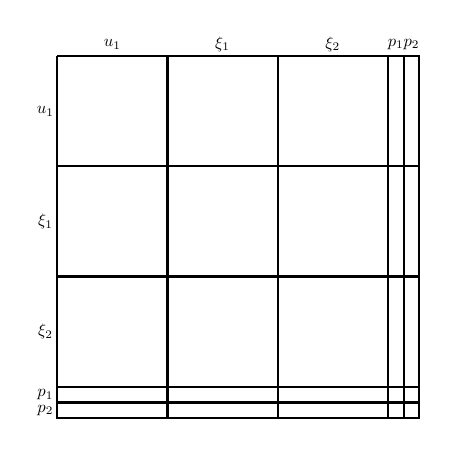
\begin{tikzpicture}[yscale=-1] 

\pgfmathsetmacro{\nt}{7};% time points
\pgfmathsetmacro{\nu}{1}; % controls
\pgfmathsetmacro{\nx}{2}; % states
\pgfmathsetmacro{\np}{2}; % parameters
\pgfmathsetmacro{\nc}{\nu + \nx}; % total continuous

%% control labels
\foreach \k in {1,...,\nu}{
	\pgfmathsetmacro{\x}{0.2*\nt*\k - 0.2/2*(\nt-1)};
	\node () at (\x,-0.05) {\scalebox{0.6}{$u_{\k}$}};
    \node () at (-0.05,\x) {\scalebox{0.6}{$u_{\k}$}};
}

%% state labels
\foreach \k in {1,...,\nx}{
	\pgfmathsetmacro{\x}{0.2*\nt*\k + 0.2*\nu*\nt - 0.2/2*(\nt-1)};
	\node () at (\x,-0.05) {\scalebox{0.6}{$\xi_{\k}$}};
    \node () at (-0.05,\x) {\scalebox{0.6}{$\xi_{\k}$}};
}

%% parameter labels
\foreach \k in {1,...,\np}{
	\pgfmathsetmacro{\x}{0.2*\k + 0.2*\nu*\nt + 0.2*\nx*\nt};
	\node () at (\x,-0.05) {\scalebox{0.6}{$p_{\k}$}};
    \node () at (-0.05,\x) {\scalebox{0.6}{$p_{\k}$}};
}


%% controls
\foreach \k in {1,...,\nu}{
	\foreach \j in {1,...,\nu}{
		\foreach \i in {1,...,\nt}{ 
        	\pgfmathsetmacro{\kk}{\k-1};
            \pgfmathsetmacro{\jj}{\j-1};
        	\pgfmathsetmacro{\x}{0.2*\i + 0.2*\kk*\nt};
            \pgfmathsetmacro{\y}{0.2*\i + 0.2*\jj*\nt};
        	\node () at (\x,\y) {\mysparsesymbol};
} 
    \pgfmathsetmacro{\kk}{\k-1};
    \pgfmathsetmacro{\jj}{\j-1};
    \pgfmathsetmacro{\x}{0.2*\kk*\nt + 0.1};
    \pgfmathsetmacro{\y}{0.2*\jj*\nt + 0.1};
	\draw[\mysparseboxcolor,thick](\x,\y) -- (\x+0.2*\nt,\y) -- (\x+0.2*\nt,\y+0.2*\nt) -- (\x,\y+0.2*\nt) -- (\x,\y);
} }

%% states
\foreach \k in {1,...,\nx}{
	\foreach \j in {1,...,\nx}{
		\foreach \i in {1,...,\nt}{ 
        	\pgfmathsetmacro{\kk}{\k-1};
            \pgfmathsetmacro{\jj}{\j-1};
        	\node () at (0.2*\i + 0.2*\kk*\nt + 0.2*\nu*\nt, 0.2*\i + 0.2*\jj*\nt + 0.2*\nu*\nt) {\mysparsesymbol};
} 
    \pgfmathsetmacro{\kk}{\k-1};
    \pgfmathsetmacro{\jj}{\j-1};
    \pgfmathsetmacro{\x}{0.2*\kk*\nt + 0.2*(\nu)*\nt + 0.1};
    \pgfmathsetmacro{\y}{0.2*\jj*\nt + 0.2*(\nu)*\nt + 0.1};
	\draw[\mysparseboxcolor,thick](\x,\y) -- (\x+0.2*\nt,\y) -- (\x+0.2*\nt,\y+0.2*\nt) -- (\x,\y+0.2*\nt) -- (\x,\y);
} }

%% parameters
\foreach \k in {1,...,\np}{
	\foreach \j in {1,...,\np}{
      \pgfmathsetmacro{\kk}{\k-1};
      \pgfmathsetmacro{\jj}{\j-1};
      \node ( ) at (0.2*\j + 0.2*\nx*\nt + 0.2*\nu*\nt, 0.2*\k + 0.2*\nx*\nt + 0.2*\nu*\nt) {\mysparsesymbol};
      \pgfmathsetmacro{\x}{0.2*\kk + 0.2*(\nu)*\nt + 0.2*\nx*\nt + 0.1};
      \pgfmathsetmacro{\y}{0.2*\jj + 0.2*(\nu)*\nt + 0.2*\nx*\nt + 0.1};
      \draw[\mysparseboxcolor,thick](\x,\y) -- (\x+0.2,\y) -- (\x+0.2,\y+0.2) -- (\x,\y+0.2) -- (\x,\y);
} }

%% states and controls
\foreach \k in {1,...,\nu}{
	\foreach \j in {1,...,\nx}{
		\foreach \i in {1,...,\nt}{ 
        	\pgfmathsetmacro{\kk}{\k-1};
            \pgfmathsetmacro{\jj}{\j-1};
        	\node () at ( 0.2*\i + 0.2*\kk*\nt , 0.2*\i + 0.2*\jj*\nt + 0.2*\nu*\nt) {\mysparsesymbol};
        	\node () at ( 0.2*\i + 0.2*\jj*\nt + 0.2*\nu*\nt, 0.2*\i + 0.2*\kk*\nt) {\mysparsesymbol};
} 
    \pgfmathsetmacro{\kk}{\k-1};
    \pgfmathsetmacro{\jj}{\j-1};
    \pgfmathsetmacro{\x}{0.2*\kk*\nt + 0.1};
    \pgfmathsetmacro{\y}{0.2*\jj*\nt + 0.2*(\nu)*\nt + 0.1};
	\draw[\mysparseboxcolor,thick](\x,\y) -- (\x+0.2*\nt,\y) -- (\x+0.2*\nt,\y+0.2*\nt) -- (\x,\y+0.2*\nt) -- (\x,\y);
    \draw[\mysparseboxcolor,thick](\y,\x) -- (\y+0.2*\nt,\x) -- (\y+0.2*\nt,\x+0.2*\nt) -- (\y,\x+0.2*\nt) -- (\y,\x);
} }

%% states and parameters
\foreach \k in {1,...,\np}{
	\foreach \j in {1,...,\nx}{
		\foreach \i in {1,...,\nt}{ 
        	\pgfmathsetmacro{\kk}{\k-1};
            \pgfmathsetmacro{\jj}{\j-1};
        	\node () at ( 0.2*\k + 0.2*\nx*\nt + 0.2*\nu*\nt, 0.2*\i + 0.2*\jj*\nt + 0.2*\nu*\nt ) {\mysparsesymbol};
            \node () at ( 0.2*\i + 0.2*\jj*\nt + 0.2*\nu*\nt, 0.2*\k + 0.2*\nx*\nt + 0.2*\nu*\nt ) {\mysparsesymbol};
} 
    \pgfmathsetmacro{\kk}{\k-1};
    \pgfmathsetmacro{\jj}{\j-1};
    \pgfmathsetmacro{\x}{0.2*\kk + 0.2*\nx*\nt + 0.2*\nu*\nt + 0.1};
    \pgfmathsetmacro{\y}{0.2*\jj*\nt + 0.2*\nu*\nt + 0.1};
	\draw[\mysparseboxcolor,thick](\x,\y) -- (\x+0.2,\y) -- (\x+0.2,\y+0.2*\nt) -- (\x,\y+0.2*\nt) -- (\x,\y);
    \draw[\mysparseboxcolor,thick](\y,\x) -- (\y+0.2*\nt,\x) -- (\y+0.2*\nt,\x+0.2) -- (\y,\x+0.2) -- (\y,\x);

} }

%% controls and parameters
\foreach \k in {1,...,\np}{
	\foreach \j in {1,...,\nu}{
		\foreach \i in {1,...,\nt}{ 
        	\pgfmathsetmacro{\kk}{\k-1};
            \pgfmathsetmacro{\jj}{\j-1};
        	\node () at ( 0.2*\k + 0.2*\nx*\nt + 0.2*\nu*\nt, 0.2*\i + 0.2*\jj*\nt ) {\mysparsesymbol};
            \node () at ( 0.2*\i + 0.2*\jj*\nt , 0.2*\k + 0.2*\nx*\nt + 0.2*\nu*\nt ) {\mysparsesymbol};
} 
    \pgfmathsetmacro{\kk}{\k-1};
    \pgfmathsetmacro{\jj}{\j-1};
    \pgfmathsetmacro{\x}{0.2*\kk + 0.2*\nx*\nt + 0.2*\nu*\nt + 0.1};
    \pgfmathsetmacro{\y}{0.2*\jj*\nt + 0.1};
	\draw[\mysparseboxcolor,thick](\x,\y) -- (\x+0.2,\y) -- (\x+0.2,\y+0.2*\nt) -- (\x,\y+0.2*\nt) -- (\x,\y);
    \draw[\mysparseboxcolor,thick](\y,\x) -- (\y+0.2*\nt,\x) -- (\y+0.2*\nt,\x+0.2) -- (\y,\x+0.2) -- (\y,\x);
} }

%% initial states
\foreach \k in {1,...,\nx}{
	\foreach \j in {1,...,\nc}{
		\foreach \i in {1,...,\nt}{ 
        	\pgfmathsetmacro{\kk}{\k-1};
            \pgfmathsetmacro{\jj}{\j-1};
        	\node () at (0.2 + 0.2*\kk*\nt + 0.2*\nu*\nt, 0.2*\i + 0.2*\jj*\nt ) {\mysparsesymbol};
            \node () at ( 0.2*\i + 0.2*\jj*\nt , 0.2 + 0.2*\kk*\nt + 0.2*\nu*\nt ) {\mysparsesymbol};
} } 
	\foreach \j in {1,...,\np}{
		\pgfmathsetmacro{\kk}{\k-1};
        \pgfmathsetmacro{\jj}{\j-1};
        \node () at ( 0.2*\k + 0.2*\nx*\nt + 0.2*\nu*\nt, 0.2 + 0.2*\jj*\nt + 0.2*\nu*\nt ) {\mysparsesymbol};
        \node () at ( 0.2 + 0.2*\jj*\nt + 0.2*\nu*\nt , 0.2*\k + 0.2*\nx*\nt + 0.2*\nu*\nt ) {\mysparsesymbol};
	}
}

%% final states
\foreach \k in {1,...,\nx}{
	\foreach \j in {1,...,\nc}{
		\foreach \i in {1,...,\nt}{ 
        	\pgfmathsetmacro{\kk}{\k-1};
            \pgfmathsetmacro{\jj}{\j-1};
        	\node () at (0.2*\nt + 0.2*\kk*\nt + 0.2*\nu*\nt, 0.2*\i + 0.2*\jj*\nt ) {\mysparsesymbol};
            \node () at ( 0.2*\i + 0.2*\jj*\nt , 0.2*\nt + 0.2*\kk*\nt + 0.2*\nu*\nt ) {\mysparsesymbol};
} } 
	\foreach \j in {1,...,\np}{
		\pgfmathsetmacro{\kk}{\k-1};
        \pgfmathsetmacro{\jj}{\j-1};
        \node () at ( 0.2*\k + 0.2*\nx*\nt + 0.2*\nu*\nt, 0.2*\nt + 0.2*\jj*\nt + 0.2*\nu*\nt ) {\mysparsesymbol};
        \node () at ( 0.2*\nt + 0.2*\jj*\nt + 0.2*\nu*\nt , 0.2*\k + 0.2*\nx*\nt + 0.2*\nu*\nt ) {\mysparsesymbol};
	}
}


























% %% states and controls
% \foreach \k in {0,...,2}{
% 	\foreach \j in {0,...,2}{
% 		\foreach \i in {1,...,5}{ 
%         	\node () at (0.2*\i + \k,0.2*\i + \j) {\mysparsesymbol};
% } } }

% %% parameters - right
% \foreach \k in {0,...,1}{
% 	\foreach \j in {0,...,2}{
% 		\foreach \i in {1,...,5}{
%         	\node ( ) at (0.2*\k + 3.2, 0.2*\i + \j) {\mysparsesymbol};
% } } }

% %% parameters - bottom
% \foreach \k in {0,...,1}{
% 	\foreach \j in {0,...,2}{
% 		\foreach \i in {1,...,5}{
%         	\node ( ) at (0.2*\i + \j, 0.2*\k + 3.2) {\mysparsesymbol};
% } } }

% %% parameters - corner
% \foreach \k in {0,...,1}{
% 	\foreach \j in {0,...,1}{
%         	\node ( ) at (0.2*\j + 3.2, 0.2*\k + 3.2) {\mysparsesymbol};
% } }

% %% initial states - bottom
% \foreach \k in {0,...,1}{
% 	\foreach \j in {0,...,2}{
% 		\foreach \i in {1,...,5}{
%         	\node ( ) at (0.2*\i + \j, \k + 1.2) {\mysparsesymbol};
% } } }

% %% final states - bottom
% \foreach \k in {0,...,1}{
% 	\foreach \j in {0,...,2}{
% 		\foreach \i in {1,...,5}{
%         	\node ( ) at (0.2*\i + \j, \k + 2.0) {\mysparsesymbol};
% } } }

% %% initial states - right
% \foreach \k in {0,...,1}{
% 	\foreach \j in {0,...,2}{
% 		\foreach \i in {1,...,5}{
%         	\node ( ) at (\k + 1.2, 0.2*\i + \j) {\mysparsesymbol};
% } } }

% %% final states - right
% \foreach \k in {0,...,1}{
% 	\foreach \j in {0,...,2}{
% 		\foreach \i in {1,...,5}{
%         	\node ( ) at (\k + 2.0, 0.2*\i + \j) {\mysparsesymbol};
% } } }


% %% draw boxes - states and controls
% \foreach \k in {0,...,2}{
% 	\foreach \j in {0,...,2}{
%     	\pgfmathsetmacro{\x}{\k + 0.1};
%     	\pgfmathsetmacro{\y}{\j + 0.1};
%         \draw[blue!70] (\x,\y) -- (\x+1,\y) -- (\x+1,\y+1) -- (\x,\y+1) -- (\x,\y);
% } }

% %% draw boxes - parameters - right
% \foreach \k in {0,...,1}{
% 	\foreach \j in {0,...,2}{
%     	\pgfmathsetmacro{\x}{0.2*\k + 0.1 + 3};
%     	\pgfmathsetmacro{\y}{\j + 0.1};
%         \draw[blue] (\x,\y) -- (\x+0.2,\y) -- (\x+0.2,\y+1) -- (\x,\y+1) -- (\x,\y);
% } }

% %% draw boxes - parameters - bottom
% \foreach \k in {0,...,2}{
% 	\foreach \j in {0,...,1}{
%     	\pgfmathsetmacro{\x}{\k + 0.1};
%     	\pgfmathsetmacro{\y}{0.2*\j + 0.1 + 3};
%         \draw[blue] (\x,\y) -- (\x+1,\y) -- (\x+1,\y+0.2) -- (\x,\y+0.2) -- (\x,\y);
% } }

% %% draw boxes - parameters - bottom
% \foreach \k in {0,...,1}{
% 	\foreach \j in {0,...,1}{
%     	\pgfmathsetmacro{\x}{0.2*\k + 0.1 + 3};
%     	\pgfmathsetmacro{\y}{0.2*\j + 0.1 + 3};
%         \draw[blue] (\x,\y) -- (\x+0.2,\y) -- (\x+0.2,\y+0.2) -- (\x,\y+0.2) -- (\x,\y);
% } }


%% final states
\foreach \k in {1,...,\nx}{
	\foreach \j in {1,...,\nc}{
		\foreach \i in {1,...,\nt}{ 
        	\pgfmathsetmacro{\kk}{\k-1};
            \pgfmathsetmacro{\jj}{\j-1};
        	\node () at (0.2*\nt + 0.2*\kk*\nt + 0.2*\nu*\nt, 0.2*\i + 0.2*\jj*\nt ) {\mytemp};
            \node () at ( 0.2*\i + 0.2*\jj*\nt , 0.2*\nt + 0.2*\kk*\nt + 0.2*\nu*\nt ) {\mytemp};
} } 
	\foreach \j in {1,...,\np}{
		\pgfmathsetmacro{\kk}{\k-1};
        \pgfmathsetmacro{\jj}{\j-1};
        \node () at ( 0.2*\k + 0.2*\nx*\nt + 0.2*\nu*\nt, 0.2*\nt + 0.2*\jj*\nt + 0.2*\nu*\nt ) {\mytemp};
        \node () at ( 0.2*\nt + 0.2*\jj*\nt + 0.2*\nu*\nt , 0.2*\k + 0.2*\nx*\nt + 0.2*\nu*\nt ) {\mytemp};
	}
}
\end{tikzpicture}
}
\end{minipage}
\caption{$\bm{L}_{5j}$ and $\bm{L}_{i5}$ terms.}
% \label{fig:}
\end{subfigure}%
\begin{subfigure}{0.33\textwidth}
\centering
\begin{minipage}{1\textwidth}
\tikzsetnextfilename{Hoff}

\centering
\resizebox{1\textwidth}{!}{
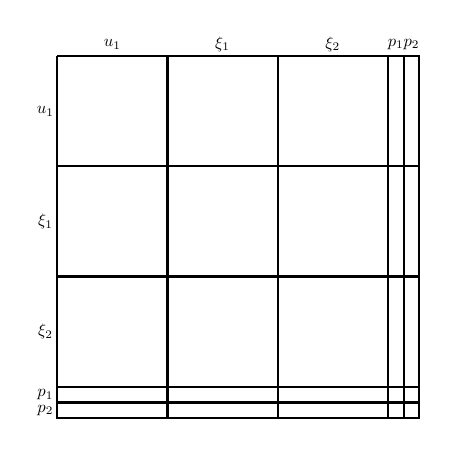
\begin{tikzpicture}[yscale=-1] 

\pgfmathsetmacro{\nt}{7};% time points
\pgfmathsetmacro{\nu}{1}; % controls
\pgfmathsetmacro{\nx}{2}; % states
\pgfmathsetmacro{\np}{2}; % parameters
\pgfmathsetmacro{\nc}{\nu + \nx}; % total continuous

%% control labels
\foreach \k in {1,...,\nu}{
	\pgfmathsetmacro{\x}{0.2*\nt*\k - 0.2/2*(\nt-1)};
	\node () at (\x,-0.05) {\scalebox{0.6}{$u_{\k}$}};
    \node () at (-0.05,\x) {\scalebox{0.6}{$u_{\k}$}};
}

%% state labels
\foreach \k in {1,...,\nx}{
	\pgfmathsetmacro{\x}{0.2*\nt*\k + 0.2*\nu*\nt - 0.2/2*(\nt-1)};
	\node () at (\x,-0.05) {\scalebox{0.6}{$\xi_{\k}$}};
    \node () at (-0.05,\x) {\scalebox{0.6}{$\xi_{\k}$}};
}

%% parameter labels
\foreach \k in {1,...,\np}{
	\pgfmathsetmacro{\x}{0.2*\k + 0.2*\nu*\nt + 0.2*\nx*\nt};
	\node () at (\x,-0.05) {\scalebox{0.6}{$p_{\k}$}};
    \node () at (-0.05,\x) {\scalebox{0.6}{$p_{\k}$}};
}


%% controls
\foreach \k in {1,...,\nu}{
	\foreach \j in {1,...,\nu}{
		\foreach \i in {1,...,\nt}{ 
        	\pgfmathsetmacro{\kk}{\k-1};
            \pgfmathsetmacro{\jj}{\j-1};
        	\pgfmathsetmacro{\x}{0.2*\i + 0.2*\kk*\nt};
            \pgfmathsetmacro{\y}{0.2*\i + 0.2*\jj*\nt};
        	\node () at (\x,\y) {\mysparsesymbol};
} 
    \pgfmathsetmacro{\kk}{\k-1};
    \pgfmathsetmacro{\jj}{\j-1};
    \pgfmathsetmacro{\x}{0.2*\kk*\nt + 0.1};
    \pgfmathsetmacro{\y}{0.2*\jj*\nt + 0.1};
	\draw[\mysparseboxcolor,thick](\x,\y) -- (\x+0.2*\nt,\y) -- (\x+0.2*\nt,\y+0.2*\nt) -- (\x,\y+0.2*\nt) -- (\x,\y);
} }

%% states
\foreach \k in {1,...,\nx}{
	\foreach \j in {1,...,\nx}{
		\foreach \i in {1,...,\nt}{ 
        	\pgfmathsetmacro{\kk}{\k-1};
            \pgfmathsetmacro{\jj}{\j-1};
        	\node () at (0.2*\i + 0.2*\kk*\nt + 0.2*\nu*\nt, 0.2*\i + 0.2*\jj*\nt + 0.2*\nu*\nt) {\mysparsesymbol};
} 
    \pgfmathsetmacro{\kk}{\k-1};
    \pgfmathsetmacro{\jj}{\j-1};
    \pgfmathsetmacro{\x}{0.2*\kk*\nt + 0.2*(\nu)*\nt + 0.1};
    \pgfmathsetmacro{\y}{0.2*\jj*\nt + 0.2*(\nu)*\nt + 0.1};
	\draw[\mysparseboxcolor,thick](\x,\y) -- (\x+0.2*\nt,\y) -- (\x+0.2*\nt,\y+0.2*\nt) -- (\x,\y+0.2*\nt) -- (\x,\y);
} }

%% parameters
\foreach \k in {1,...,\np}{
	\foreach \j in {1,...,\np}{
      \pgfmathsetmacro{\kk}{\k-1};
      \pgfmathsetmacro{\jj}{\j-1};
      \node ( ) at (0.2*\j + 0.2*\nx*\nt + 0.2*\nu*\nt, 0.2*\k + 0.2*\nx*\nt + 0.2*\nu*\nt) {\mysparsesymbol};
      \pgfmathsetmacro{\x}{0.2*\kk + 0.2*(\nu)*\nt + 0.2*\nx*\nt + 0.1};
      \pgfmathsetmacro{\y}{0.2*\jj + 0.2*(\nu)*\nt + 0.2*\nx*\nt + 0.1};
      \draw[\mysparseboxcolor,thick](\x,\y) -- (\x+0.2,\y) -- (\x+0.2,\y+0.2) -- (\x,\y+0.2) -- (\x,\y);
} }

%% states and controls
\foreach \k in {1,...,\nu}{
	\foreach \j in {1,...,\nx}{
		\foreach \i in {1,...,\nt}{ 
        	\pgfmathsetmacro{\kk}{\k-1};
            \pgfmathsetmacro{\jj}{\j-1};
        	\node () at ( 0.2*\i + 0.2*\kk*\nt , 0.2*\i + 0.2*\jj*\nt + 0.2*\nu*\nt) {\mysparsesymbol};
        	\node () at ( 0.2*\i + 0.2*\jj*\nt + 0.2*\nu*\nt, 0.2*\i + 0.2*\kk*\nt) {\mysparsesymbol};
} 
    \pgfmathsetmacro{\kk}{\k-1};
    \pgfmathsetmacro{\jj}{\j-1};
    \pgfmathsetmacro{\x}{0.2*\kk*\nt + 0.1};
    \pgfmathsetmacro{\y}{0.2*\jj*\nt + 0.2*(\nu)*\nt + 0.1};
	\draw[\mysparseboxcolor,thick](\x,\y) -- (\x+0.2*\nt,\y) -- (\x+0.2*\nt,\y+0.2*\nt) -- (\x,\y+0.2*\nt) -- (\x,\y);
    \draw[\mysparseboxcolor,thick](\y,\x) -- (\y+0.2*\nt,\x) -- (\y+0.2*\nt,\x+0.2*\nt) -- (\y,\x+0.2*\nt) -- (\y,\x);
} }

%% states and parameters
\foreach \k in {1,...,\np}{
	\foreach \j in {1,...,\nx}{
		\foreach \i in {1,...,\nt}{ 
        	\pgfmathsetmacro{\kk}{\k-1};
            \pgfmathsetmacro{\jj}{\j-1};
        	\node () at ( 0.2*\k + 0.2*\nx*\nt + 0.2*\nu*\nt, 0.2*\i + 0.2*\jj*\nt + 0.2*\nu*\nt ) {\mysparsesymbol};
            \node () at ( 0.2*\i + 0.2*\jj*\nt + 0.2*\nu*\nt, 0.2*\k + 0.2*\nx*\nt + 0.2*\nu*\nt ) {\mysparsesymbol};
} 
    \pgfmathsetmacro{\kk}{\k-1};
    \pgfmathsetmacro{\jj}{\j-1};
    \pgfmathsetmacro{\x}{0.2*\kk + 0.2*\nx*\nt + 0.2*\nu*\nt + 0.1};
    \pgfmathsetmacro{\y}{0.2*\jj*\nt + 0.2*\nu*\nt + 0.1};
	\draw[\mysparseboxcolor,thick](\x,\y) -- (\x+0.2,\y) -- (\x+0.2,\y+0.2*\nt) -- (\x,\y+0.2*\nt) -- (\x,\y);
    \draw[\mysparseboxcolor,thick](\y,\x) -- (\y+0.2*\nt,\x) -- (\y+0.2*\nt,\x+0.2) -- (\y,\x+0.2) -- (\y,\x);

} }

%% controls and parameters
\foreach \k in {1,...,\np}{
	\foreach \j in {1,...,\nu}{
		\foreach \i in {1,...,\nt}{ 
        	\pgfmathsetmacro{\kk}{\k-1};
            \pgfmathsetmacro{\jj}{\j-1};
        	\node () at ( 0.2*\k + 0.2*\nx*\nt + 0.2*\nu*\nt, 0.2*\i + 0.2*\jj*\nt ) {\mysparsesymbol};
            \node () at ( 0.2*\i + 0.2*\jj*\nt , 0.2*\k + 0.2*\nx*\nt + 0.2*\nu*\nt ) {\mysparsesymbol};
} 
    \pgfmathsetmacro{\kk}{\k-1};
    \pgfmathsetmacro{\jj}{\j-1};
    \pgfmathsetmacro{\x}{0.2*\kk + 0.2*\nx*\nt + 0.2*\nu*\nt + 0.1};
    \pgfmathsetmacro{\y}{0.2*\jj*\nt + 0.1};
	\draw[\mysparseboxcolor,thick](\x,\y) -- (\x+0.2,\y) -- (\x+0.2,\y+0.2*\nt) -- (\x,\y+0.2*\nt) -- (\x,\y);
    \draw[\mysparseboxcolor,thick](\y,\x) -- (\y+0.2*\nt,\x) -- (\y+0.2*\nt,\x+0.2) -- (\y,\x+0.2) -- (\y,\x);
} }

%% initial states
\foreach \k in {1,...,\nx}{
	\foreach \j in {1,...,\nc}{
		\foreach \i in {1,...,\nt}{ 
        	\pgfmathsetmacro{\kk}{\k-1};
            \pgfmathsetmacro{\jj}{\j-1};
        	\node () at (0.2 + 0.2*\kk*\nt + 0.2*\nu*\nt, 0.2*\i + 0.2*\jj*\nt ) {\mysparsesymbol};
            \node () at ( 0.2*\i + 0.2*\jj*\nt , 0.2 + 0.2*\kk*\nt + 0.2*\nu*\nt ) {\mysparsesymbol};
} } 
	\foreach \j in {1,...,\np}{
		\pgfmathsetmacro{\kk}{\k-1};
        \pgfmathsetmacro{\jj}{\j-1};
        \node () at ( 0.2*\k + 0.2*\nx*\nt + 0.2*\nu*\nt, 0.2 + 0.2*\jj*\nt + 0.2*\nu*\nt ) {\mysparsesymbol};
        \node () at ( 0.2 + 0.2*\jj*\nt + 0.2*\nu*\nt , 0.2*\k + 0.2*\nx*\nt + 0.2*\nu*\nt ) {\mysparsesymbol};
	}
}

%% final states
\foreach \k in {1,...,\nx}{
	\foreach \j in {1,...,\nc}{
		\foreach \i in {1,...,\nt}{ 
        	\pgfmathsetmacro{\kk}{\k-1};
            \pgfmathsetmacro{\jj}{\j-1};
        	\node () at (0.2*\nt + 0.2*\kk*\nt + 0.2*\nu*\nt, 0.2*\i + 0.2*\jj*\nt ) {\mysparsesymbol};
            \node () at ( 0.2*\i + 0.2*\jj*\nt , 0.2*\nt + 0.2*\kk*\nt + 0.2*\nu*\nt ) {\mysparsesymbol};
} } 
	\foreach \j in {1,...,\np}{
		\pgfmathsetmacro{\kk}{\k-1};
        \pgfmathsetmacro{\jj}{\j-1};
        \node () at ( 0.2*\k + 0.2*\nx*\nt + 0.2*\nu*\nt, 0.2*\nt + 0.2*\jj*\nt + 0.2*\nu*\nt ) {\mysparsesymbol};
        \node () at ( 0.2*\nt + 0.2*\jj*\nt + 0.2*\nu*\nt , 0.2*\k + 0.2*\nx*\nt + 0.2*\nu*\nt ) {\mysparsesymbol};
	}
}


























% %% states and controls
% \foreach \k in {0,...,2}{
% 	\foreach \j in {0,...,2}{
% 		\foreach \i in {1,...,5}{ 
%         	\node () at (0.2*\i + \k,0.2*\i + \j) {\mysparsesymbol};
% } } }

% %% parameters - right
% \foreach \k in {0,...,1}{
% 	\foreach \j in {0,...,2}{
% 		\foreach \i in {1,...,5}{
%         	\node ( ) at (0.2*\k + 3.2, 0.2*\i + \j) {\mysparsesymbol};
% } } }

% %% parameters - bottom
% \foreach \k in {0,...,1}{
% 	\foreach \j in {0,...,2}{
% 		\foreach \i in {1,...,5}{
%         	\node ( ) at (0.2*\i + \j, 0.2*\k + 3.2) {\mysparsesymbol};
% } } }

% %% parameters - corner
% \foreach \k in {0,...,1}{
% 	\foreach \j in {0,...,1}{
%         	\node ( ) at (0.2*\j + 3.2, 0.2*\k + 3.2) {\mysparsesymbol};
% } }

% %% initial states - bottom
% \foreach \k in {0,...,1}{
% 	\foreach \j in {0,...,2}{
% 		\foreach \i in {1,...,5}{
%         	\node ( ) at (0.2*\i + \j, \k + 1.2) {\mysparsesymbol};
% } } }

% %% final states - bottom
% \foreach \k in {0,...,1}{
% 	\foreach \j in {0,...,2}{
% 		\foreach \i in {1,...,5}{
%         	\node ( ) at (0.2*\i + \j, \k + 2.0) {\mysparsesymbol};
% } } }

% %% initial states - right
% \foreach \k in {0,...,1}{
% 	\foreach \j in {0,...,2}{
% 		\foreach \i in {1,...,5}{
%         	\node ( ) at (\k + 1.2, 0.2*\i + \j) {\mysparsesymbol};
% } } }

% %% final states - right
% \foreach \k in {0,...,1}{
% 	\foreach \j in {0,...,2}{
% 		\foreach \i in {1,...,5}{
%         	\node ( ) at (\k + 2.0, 0.2*\i + \j) {\mysparsesymbol};
% } } }


% %% draw boxes - states and controls
% \foreach \k in {0,...,2}{
% 	\foreach \j in {0,...,2}{
%     	\pgfmathsetmacro{\x}{\k + 0.1};
%     	\pgfmathsetmacro{\y}{\j + 0.1};
%         \draw[blue!70] (\x,\y) -- (\x+1,\y) -- (\x+1,\y+1) -- (\x,\y+1) -- (\x,\y);
% } }

% %% draw boxes - parameters - right
% \foreach \k in {0,...,1}{
% 	\foreach \j in {0,...,2}{
%     	\pgfmathsetmacro{\x}{0.2*\k + 0.1 + 3};
%     	\pgfmathsetmacro{\y}{\j + 0.1};
%         \draw[blue] (\x,\y) -- (\x+0.2,\y) -- (\x+0.2,\y+1) -- (\x,\y+1) -- (\x,\y);
% } }

% %% draw boxes - parameters - bottom
% \foreach \k in {0,...,2}{
% 	\foreach \j in {0,...,1}{
%     	\pgfmathsetmacro{\x}{\k + 0.1};
%     	\pgfmathsetmacro{\y}{0.2*\j + 0.1 + 3};
%         \draw[blue] (\x,\y) -- (\x+1,\y) -- (\x+1,\y+0.2) -- (\x,\y+0.2) -- (\x,\y);
% } }

% %% draw boxes - parameters - bottom
% \foreach \k in {0,...,1}{
% 	\foreach \j in {0,...,1}{
%     	\pgfmathsetmacro{\x}{0.2*\k + 0.1 + 3};
%     	\pgfmathsetmacro{\y}{0.2*\j + 0.1 + 3};
%         \draw[blue] (\x,\y) -- (\x+0.2,\y) -- (\x+0.2,\y+0.2) -- (\x,\y+0.2) -- (\x,\y);
% } }


%% states and controls
\foreach \k in {1,...,\nu}{
	\foreach \j in {1,...,\nx}{
		\foreach \i in {1,...,\nt}{ 
        	\pgfmathsetmacro{\kk}{\k-1};
            \pgfmathsetmacro{\jj}{\j-1};
        	\node () at ( 0.2*\i + 0.2*\kk*\nt , 0.2*\i + 0.2*\jj*\nt + 0.2*\nu*\nt) {\mytemp};
        	\node () at ( 0.2*\i + 0.2*\jj*\nt + 0.2*\nu*\nt, 0.2*\i + 0.2*\kk*\nt) {\mytemp};
} } }

%% states and parameters
\foreach \k in {1,...,\np}{
	\foreach \j in {1,...,\nx}{
		\foreach \i in {1,...,\nt}{ 
        	\pgfmathsetmacro{\kk}{\k-1};
            \pgfmathsetmacro{\jj}{\j-1};
        	\node () at ( 0.2*\k + 0.2*\nx*\nt + 0.2*\nu*\nt, 0.2*\i + 0.2*\jj*\nt + 0.2*\nu*\nt ) {\mytemp};
            \node () at ( 0.2*\i + 0.2*\jj*\nt + 0.2*\nu*\nt, 0.2*\k + 0.2*\nx*\nt + 0.2*\nu*\nt ) {\mytemp};
} } }

%% controls and parameters
\foreach \k in {1,...,\np}{
	\foreach \j in {1,...,\nu}{
		\foreach \i in {1,...,\nt}{ 
        	\pgfmathsetmacro{\kk}{\k-1};
            \pgfmathsetmacro{\jj}{\j-1};
        	\node () at ( 0.2*\k + 0.2*\nx*\nt + 0.2*\nu*\nt, 0.2*\i + 0.2*\jj*\nt ) {\mytemp};
            \node () at ( 0.2*\i + 0.2*\jj*\nt , 0.2*\k + 0.2*\nx*\nt + 0.2*\nu*\nt ) {\mytemp};
} } }

\end{tikzpicture}
}
\end{minipage}
\caption{Remaining terms.}
% \label{fig:}
\end{subfigure}%

\caption{Sparsity pattern of $\mathbf{H}$ matrix for all considered methods except CQHS.}
\label{fig:figsparsityHSS}
\end{figure}


% \begin{figure}[h]

% \centering

% \subfloat[(a) $\bm{L}_{11}$ terms.]{\label{fig:L11}
% 	\begin{minipage}{0.33\textwidth}
% 	\tikzsetnextfilename{Huu}

\centering
\resizebox{1\textwidth}{!}{
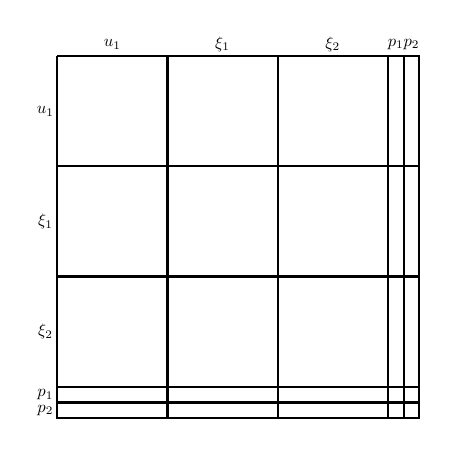
\begin{tikzpicture}[yscale=-1] 

\pgfmathsetmacro{\nt}{7};% time points
\pgfmathsetmacro{\nu}{1}; % controls
\pgfmathsetmacro{\nx}{2}; % states
\pgfmathsetmacro{\np}{2}; % parameters
\pgfmathsetmacro{\nc}{\nu + \nx}; % total continuous

%% control labels
\foreach \k in {1,...,\nu}{
	\pgfmathsetmacro{\x}{0.2*\nt*\k - 0.2/2*(\nt-1)};
	\node () at (\x,-0.05) {\scalebox{0.6}{$u_{\k}$}};
    \node () at (-0.05,\x) {\scalebox{0.6}{$u_{\k}$}};
}

%% state labels
\foreach \k in {1,...,\nx}{
	\pgfmathsetmacro{\x}{0.2*\nt*\k + 0.2*\nu*\nt - 0.2/2*(\nt-1)};
	\node () at (\x,-0.05) {\scalebox{0.6}{$\xi_{\k}$}};
    \node () at (-0.05,\x) {\scalebox{0.6}{$\xi_{\k}$}};
}

%% parameter labels
\foreach \k in {1,...,\np}{
	\pgfmathsetmacro{\x}{0.2*\k + 0.2*\nu*\nt + 0.2*\nx*\nt};
	\node () at (\x,-0.05) {\scalebox{0.6}{$p_{\k}$}};
    \node () at (-0.05,\x) {\scalebox{0.6}{$p_{\k}$}};
}


%% controls
\foreach \k in {1,...,\nu}{
	\foreach \j in {1,...,\nu}{
		\foreach \i in {1,...,\nt}{ 
        	\pgfmathsetmacro{\kk}{\k-1};
            \pgfmathsetmacro{\jj}{\j-1};
        	\pgfmathsetmacro{\x}{0.2*\i + 0.2*\kk*\nt};
            \pgfmathsetmacro{\y}{0.2*\i + 0.2*\jj*\nt};
        	\node () at (\x,\y) {\mysparsesymbol};
} 
    \pgfmathsetmacro{\kk}{\k-1};
    \pgfmathsetmacro{\jj}{\j-1};
    \pgfmathsetmacro{\x}{0.2*\kk*\nt + 0.1};
    \pgfmathsetmacro{\y}{0.2*\jj*\nt + 0.1};
	\draw[\mysparseboxcolor,thick](\x,\y) -- (\x+0.2*\nt,\y) -- (\x+0.2*\nt,\y+0.2*\nt) -- (\x,\y+0.2*\nt) -- (\x,\y);
} }

%% states
\foreach \k in {1,...,\nx}{
	\foreach \j in {1,...,\nx}{
		\foreach \i in {1,...,\nt}{ 
        	\pgfmathsetmacro{\kk}{\k-1};
            \pgfmathsetmacro{\jj}{\j-1};
        	\node () at (0.2*\i + 0.2*\kk*\nt + 0.2*\nu*\nt, 0.2*\i + 0.2*\jj*\nt + 0.2*\nu*\nt) {\mysparsesymbol};
} 
    \pgfmathsetmacro{\kk}{\k-1};
    \pgfmathsetmacro{\jj}{\j-1};
    \pgfmathsetmacro{\x}{0.2*\kk*\nt + 0.2*(\nu)*\nt + 0.1};
    \pgfmathsetmacro{\y}{0.2*\jj*\nt + 0.2*(\nu)*\nt + 0.1};
	\draw[\mysparseboxcolor,thick](\x,\y) -- (\x+0.2*\nt,\y) -- (\x+0.2*\nt,\y+0.2*\nt) -- (\x,\y+0.2*\nt) -- (\x,\y);
} }

%% parameters
\foreach \k in {1,...,\np}{
	\foreach \j in {1,...,\np}{
      \pgfmathsetmacro{\kk}{\k-1};
      \pgfmathsetmacro{\jj}{\j-1};
      \node ( ) at (0.2*\j + 0.2*\nx*\nt + 0.2*\nu*\nt, 0.2*\k + 0.2*\nx*\nt + 0.2*\nu*\nt) {\mysparsesymbol};
      \pgfmathsetmacro{\x}{0.2*\kk + 0.2*(\nu)*\nt + 0.2*\nx*\nt + 0.1};
      \pgfmathsetmacro{\y}{0.2*\jj + 0.2*(\nu)*\nt + 0.2*\nx*\nt + 0.1};
      \draw[\mysparseboxcolor,thick](\x,\y) -- (\x+0.2,\y) -- (\x+0.2,\y+0.2) -- (\x,\y+0.2) -- (\x,\y);
} }

%% states and controls
\foreach \k in {1,...,\nu}{
	\foreach \j in {1,...,\nx}{
		\foreach \i in {1,...,\nt}{ 
        	\pgfmathsetmacro{\kk}{\k-1};
            \pgfmathsetmacro{\jj}{\j-1};
        	\node () at ( 0.2*\i + 0.2*\kk*\nt , 0.2*\i + 0.2*\jj*\nt + 0.2*\nu*\nt) {\mysparsesymbol};
        	\node () at ( 0.2*\i + 0.2*\jj*\nt + 0.2*\nu*\nt, 0.2*\i + 0.2*\kk*\nt) {\mysparsesymbol};
} 
    \pgfmathsetmacro{\kk}{\k-1};
    \pgfmathsetmacro{\jj}{\j-1};
    \pgfmathsetmacro{\x}{0.2*\kk*\nt + 0.1};
    \pgfmathsetmacro{\y}{0.2*\jj*\nt + 0.2*(\nu)*\nt + 0.1};
	\draw[\mysparseboxcolor,thick](\x,\y) -- (\x+0.2*\nt,\y) -- (\x+0.2*\nt,\y+0.2*\nt) -- (\x,\y+0.2*\nt) -- (\x,\y);
    \draw[\mysparseboxcolor,thick](\y,\x) -- (\y+0.2*\nt,\x) -- (\y+0.2*\nt,\x+0.2*\nt) -- (\y,\x+0.2*\nt) -- (\y,\x);
} }

%% states and parameters
\foreach \k in {1,...,\np}{
	\foreach \j in {1,...,\nx}{
		\foreach \i in {1,...,\nt}{ 
        	\pgfmathsetmacro{\kk}{\k-1};
            \pgfmathsetmacro{\jj}{\j-1};
        	\node () at ( 0.2*\k + 0.2*\nx*\nt + 0.2*\nu*\nt, 0.2*\i + 0.2*\jj*\nt + 0.2*\nu*\nt ) {\mysparsesymbol};
            \node () at ( 0.2*\i + 0.2*\jj*\nt + 0.2*\nu*\nt, 0.2*\k + 0.2*\nx*\nt + 0.2*\nu*\nt ) {\mysparsesymbol};
} 
    \pgfmathsetmacro{\kk}{\k-1};
    \pgfmathsetmacro{\jj}{\j-1};
    \pgfmathsetmacro{\x}{0.2*\kk + 0.2*\nx*\nt + 0.2*\nu*\nt + 0.1};
    \pgfmathsetmacro{\y}{0.2*\jj*\nt + 0.2*\nu*\nt + 0.1};
	\draw[\mysparseboxcolor,thick](\x,\y) -- (\x+0.2,\y) -- (\x+0.2,\y+0.2*\nt) -- (\x,\y+0.2*\nt) -- (\x,\y);
    \draw[\mysparseboxcolor,thick](\y,\x) -- (\y+0.2*\nt,\x) -- (\y+0.2*\nt,\x+0.2) -- (\y,\x+0.2) -- (\y,\x);

} }

%% controls and parameters
\foreach \k in {1,...,\np}{
	\foreach \j in {1,...,\nu}{
		\foreach \i in {1,...,\nt}{ 
        	\pgfmathsetmacro{\kk}{\k-1};
            \pgfmathsetmacro{\jj}{\j-1};
        	\node () at ( 0.2*\k + 0.2*\nx*\nt + 0.2*\nu*\nt, 0.2*\i + 0.2*\jj*\nt ) {\mysparsesymbol};
            \node () at ( 0.2*\i + 0.2*\jj*\nt , 0.2*\k + 0.2*\nx*\nt + 0.2*\nu*\nt ) {\mysparsesymbol};
} 
    \pgfmathsetmacro{\kk}{\k-1};
    \pgfmathsetmacro{\jj}{\j-1};
    \pgfmathsetmacro{\x}{0.2*\kk + 0.2*\nx*\nt + 0.2*\nu*\nt + 0.1};
    \pgfmathsetmacro{\y}{0.2*\jj*\nt + 0.1};
	\draw[\mysparseboxcolor,thick](\x,\y) -- (\x+0.2,\y) -- (\x+0.2,\y+0.2*\nt) -- (\x,\y+0.2*\nt) -- (\x,\y);
    \draw[\mysparseboxcolor,thick](\y,\x) -- (\y+0.2*\nt,\x) -- (\y+0.2*\nt,\x+0.2) -- (\y,\x+0.2) -- (\y,\x);
} }

%% initial states
\foreach \k in {1,...,\nx}{
	\foreach \j in {1,...,\nc}{
		\foreach \i in {1,...,\nt}{ 
        	\pgfmathsetmacro{\kk}{\k-1};
            \pgfmathsetmacro{\jj}{\j-1};
        	\node () at (0.2 + 0.2*\kk*\nt + 0.2*\nu*\nt, 0.2*\i + 0.2*\jj*\nt ) {\mysparsesymbol};
            \node () at ( 0.2*\i + 0.2*\jj*\nt , 0.2 + 0.2*\kk*\nt + 0.2*\nu*\nt ) {\mysparsesymbol};
} } 
	\foreach \j in {1,...,\np}{
		\pgfmathsetmacro{\kk}{\k-1};
        \pgfmathsetmacro{\jj}{\j-1};
        \node () at ( 0.2*\k + 0.2*\nx*\nt + 0.2*\nu*\nt, 0.2 + 0.2*\jj*\nt + 0.2*\nu*\nt ) {\mysparsesymbol};
        \node () at ( 0.2 + 0.2*\jj*\nt + 0.2*\nu*\nt , 0.2*\k + 0.2*\nx*\nt + 0.2*\nu*\nt ) {\mysparsesymbol};
	}
}

%% final states
\foreach \k in {1,...,\nx}{
	\foreach \j in {1,...,\nc}{
		\foreach \i in {1,...,\nt}{ 
        	\pgfmathsetmacro{\kk}{\k-1};
            \pgfmathsetmacro{\jj}{\j-1};
        	\node () at (0.2*\nt + 0.2*\kk*\nt + 0.2*\nu*\nt, 0.2*\i + 0.2*\jj*\nt ) {\mysparsesymbol};
            \node () at ( 0.2*\i + 0.2*\jj*\nt , 0.2*\nt + 0.2*\kk*\nt + 0.2*\nu*\nt ) {\mysparsesymbol};
} } 
	\foreach \j in {1,...,\np}{
		\pgfmathsetmacro{\kk}{\k-1};
        \pgfmathsetmacro{\jj}{\j-1};
        \node () at ( 0.2*\k + 0.2*\nx*\nt + 0.2*\nu*\nt, 0.2*\nt + 0.2*\jj*\nt + 0.2*\nu*\nt ) {\mysparsesymbol};
        \node () at ( 0.2*\nt + 0.2*\jj*\nt + 0.2*\nu*\nt , 0.2*\k + 0.2*\nx*\nt + 0.2*\nu*\nt ) {\mysparsesymbol};
	}
}


























% %% states and controls
% \foreach \k in {0,...,2}{
% 	\foreach \j in {0,...,2}{
% 		\foreach \i in {1,...,5}{ 
%         	\node () at (0.2*\i + \k,0.2*\i + \j) {\mysparsesymbol};
% } } }

% %% parameters - right
% \foreach \k in {0,...,1}{
% 	\foreach \j in {0,...,2}{
% 		\foreach \i in {1,...,5}{
%         	\node ( ) at (0.2*\k + 3.2, 0.2*\i + \j) {\mysparsesymbol};
% } } }

% %% parameters - bottom
% \foreach \k in {0,...,1}{
% 	\foreach \j in {0,...,2}{
% 		\foreach \i in {1,...,5}{
%         	\node ( ) at (0.2*\i + \j, 0.2*\k + 3.2) {\mysparsesymbol};
% } } }

% %% parameters - corner
% \foreach \k in {0,...,1}{
% 	\foreach \j in {0,...,1}{
%         	\node ( ) at (0.2*\j + 3.2, 0.2*\k + 3.2) {\mysparsesymbol};
% } }

% %% initial states - bottom
% \foreach \k in {0,...,1}{
% 	\foreach \j in {0,...,2}{
% 		\foreach \i in {1,...,5}{
%         	\node ( ) at (0.2*\i + \j, \k + 1.2) {\mysparsesymbol};
% } } }

% %% final states - bottom
% \foreach \k in {0,...,1}{
% 	\foreach \j in {0,...,2}{
% 		\foreach \i in {1,...,5}{
%         	\node ( ) at (0.2*\i + \j, \k + 2.0) {\mysparsesymbol};
% } } }

% %% initial states - right
% \foreach \k in {0,...,1}{
% 	\foreach \j in {0,...,2}{
% 		\foreach \i in {1,...,5}{
%         	\node ( ) at (\k + 1.2, 0.2*\i + \j) {\mysparsesymbol};
% } } }

% %% final states - right
% \foreach \k in {0,...,1}{
% 	\foreach \j in {0,...,2}{
% 		\foreach \i in {1,...,5}{
%         	\node ( ) at (\k + 2.0, 0.2*\i + \j) {\mysparsesymbol};
% } } }


% %% draw boxes - states and controls
% \foreach \k in {0,...,2}{
% 	\foreach \j in {0,...,2}{
%     	\pgfmathsetmacro{\x}{\k + 0.1};
%     	\pgfmathsetmacro{\y}{\j + 0.1};
%         \draw[blue!70] (\x,\y) -- (\x+1,\y) -- (\x+1,\y+1) -- (\x,\y+1) -- (\x,\y);
% } }

% %% draw boxes - parameters - right
% \foreach \k in {0,...,1}{
% 	\foreach \j in {0,...,2}{
%     	\pgfmathsetmacro{\x}{0.2*\k + 0.1 + 3};
%     	\pgfmathsetmacro{\y}{\j + 0.1};
%         \draw[blue] (\x,\y) -- (\x+0.2,\y) -- (\x+0.2,\y+1) -- (\x,\y+1) -- (\x,\y);
% } }

% %% draw boxes - parameters - bottom
% \foreach \k in {0,...,2}{
% 	\foreach \j in {0,...,1}{
%     	\pgfmathsetmacro{\x}{\k + 0.1};
%     	\pgfmathsetmacro{\y}{0.2*\j + 0.1 + 3};
%         \draw[blue] (\x,\y) -- (\x+1,\y) -- (\x+1,\y+0.2) -- (\x,\y+0.2) -- (\x,\y);
% } }

% %% draw boxes - parameters - bottom
% \foreach \k in {0,...,1}{
% 	\foreach \j in {0,...,1}{
%     	\pgfmathsetmacro{\x}{0.2*\k + 0.1 + 3};
%     	\pgfmathsetmacro{\y}{0.2*\j + 0.1 + 3};
%         \draw[blue] (\x,\y) -- (\x+0.2,\y) -- (\x+0.2,\y+0.2) -- (\x,\y+0.2) -- (\x,\y);
% } }


%% controls
\foreach \k in {1,...,\nu}{
	\foreach \j in {1,...,\nu}{
		\foreach \i in {1,...,\nt}{ 
        	\pgfmathsetmacro{\kk}{\k-1};
            \pgfmathsetmacro{\jj}{\j-1};
        	\pgfmathsetmacro{\x}{0.2*\i + 0.2*\kk*\nt};
            \pgfmathsetmacro{\y}{0.2*\i + 0.2*\jj*\nt};
        	\node () at (\x,\y) {\mytemp};
} } }
\end{tikzpicture}
}
% 	\end{minipage}
% }%
% \subfloat[(b) $\bm{L}_{22}$ terms.]{\label{fig:L22}
% 	\begin{minipage}{0.33\textwidth}
% 	\input{../ch5/sparsity/Hxx}
% 	\end{minipage}
% }%
% \subfloat[(c) $\bm{L}_{33}$ terms.]{
% 	\begin{minipage}{0.33\textwidth}
% 	\tikzsetnextfilename{Hpp}

\centering
\resizebox{1\textwidth}{!}{
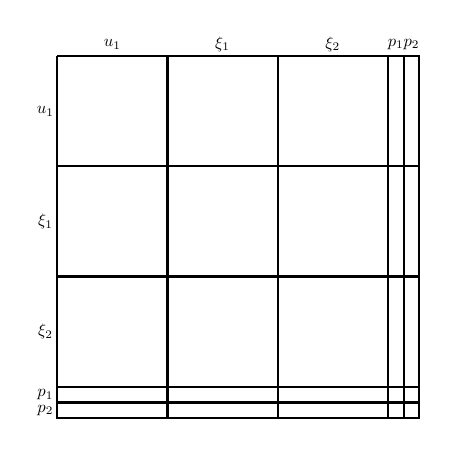
\begin{tikzpicture}[yscale=-1] 

\pgfmathsetmacro{\nt}{7};% time points
\pgfmathsetmacro{\nu}{1}; % controls
\pgfmathsetmacro{\nx}{2}; % states
\pgfmathsetmacro{\np}{2}; % parameters
\pgfmathsetmacro{\nc}{\nu + \nx}; % total continuous

%% control labels
\foreach \k in {1,...,\nu}{
	\pgfmathsetmacro{\x}{0.2*\nt*\k - 0.2/2*(\nt-1)};
	\node () at (\x,-0.05) {\scalebox{0.6}{$u_{\k}$}};
    \node () at (-0.05,\x) {\scalebox{0.6}{$u_{\k}$}};
}

%% state labels
\foreach \k in {1,...,\nx}{
	\pgfmathsetmacro{\x}{0.2*\nt*\k + 0.2*\nu*\nt - 0.2/2*(\nt-1)};
	\node () at (\x,-0.05) {\scalebox{0.6}{$\xi_{\k}$}};
    \node () at (-0.05,\x) {\scalebox{0.6}{$\xi_{\k}$}};
}

%% parameter labels
\foreach \k in {1,...,\np}{
	\pgfmathsetmacro{\x}{0.2*\k + 0.2*\nu*\nt + 0.2*\nx*\nt};
	\node () at (\x,-0.05) {\scalebox{0.6}{$p_{\k}$}};
    \node () at (-0.05,\x) {\scalebox{0.6}{$p_{\k}$}};
}


%% controls
\foreach \k in {1,...,\nu}{
	\foreach \j in {1,...,\nu}{
		\foreach \i in {1,...,\nt}{ 
        	\pgfmathsetmacro{\kk}{\k-1};
            \pgfmathsetmacro{\jj}{\j-1};
        	\pgfmathsetmacro{\x}{0.2*\i + 0.2*\kk*\nt};
            \pgfmathsetmacro{\y}{0.2*\i + 0.2*\jj*\nt};
        	\node () at (\x,\y) {\mysparsesymbol};
} 
    \pgfmathsetmacro{\kk}{\k-1};
    \pgfmathsetmacro{\jj}{\j-1};
    \pgfmathsetmacro{\x}{0.2*\kk*\nt + 0.1};
    \pgfmathsetmacro{\y}{0.2*\jj*\nt + 0.1};
	\draw[\mysparseboxcolor,thick](\x,\y) -- (\x+0.2*\nt,\y) -- (\x+0.2*\nt,\y+0.2*\nt) -- (\x,\y+0.2*\nt) -- (\x,\y);
} }

%% states
\foreach \k in {1,...,\nx}{
	\foreach \j in {1,...,\nx}{
		\foreach \i in {1,...,\nt}{ 
        	\pgfmathsetmacro{\kk}{\k-1};
            \pgfmathsetmacro{\jj}{\j-1};
        	\node () at (0.2*\i + 0.2*\kk*\nt + 0.2*\nu*\nt, 0.2*\i + 0.2*\jj*\nt + 0.2*\nu*\nt) {\mysparsesymbol};
} 
    \pgfmathsetmacro{\kk}{\k-1};
    \pgfmathsetmacro{\jj}{\j-1};
    \pgfmathsetmacro{\x}{0.2*\kk*\nt + 0.2*(\nu)*\nt + 0.1};
    \pgfmathsetmacro{\y}{0.2*\jj*\nt + 0.2*(\nu)*\nt + 0.1};
	\draw[\mysparseboxcolor,thick](\x,\y) -- (\x+0.2*\nt,\y) -- (\x+0.2*\nt,\y+0.2*\nt) -- (\x,\y+0.2*\nt) -- (\x,\y);
} }

%% parameters
\foreach \k in {1,...,\np}{
	\foreach \j in {1,...,\np}{
      \pgfmathsetmacro{\kk}{\k-1};
      \pgfmathsetmacro{\jj}{\j-1};
      \node ( ) at (0.2*\j + 0.2*\nx*\nt + 0.2*\nu*\nt, 0.2*\k + 0.2*\nx*\nt + 0.2*\nu*\nt) {\mysparsesymbol};
      \pgfmathsetmacro{\x}{0.2*\kk + 0.2*(\nu)*\nt + 0.2*\nx*\nt + 0.1};
      \pgfmathsetmacro{\y}{0.2*\jj + 0.2*(\nu)*\nt + 0.2*\nx*\nt + 0.1};
      \draw[\mysparseboxcolor,thick](\x,\y) -- (\x+0.2,\y) -- (\x+0.2,\y+0.2) -- (\x,\y+0.2) -- (\x,\y);
} }

%% states and controls
\foreach \k in {1,...,\nu}{
	\foreach \j in {1,...,\nx}{
		\foreach \i in {1,...,\nt}{ 
        	\pgfmathsetmacro{\kk}{\k-1};
            \pgfmathsetmacro{\jj}{\j-1};
        	\node () at ( 0.2*\i + 0.2*\kk*\nt , 0.2*\i + 0.2*\jj*\nt + 0.2*\nu*\nt) {\mysparsesymbol};
        	\node () at ( 0.2*\i + 0.2*\jj*\nt + 0.2*\nu*\nt, 0.2*\i + 0.2*\kk*\nt) {\mysparsesymbol};
} 
    \pgfmathsetmacro{\kk}{\k-1};
    \pgfmathsetmacro{\jj}{\j-1};
    \pgfmathsetmacro{\x}{0.2*\kk*\nt + 0.1};
    \pgfmathsetmacro{\y}{0.2*\jj*\nt + 0.2*(\nu)*\nt + 0.1};
	\draw[\mysparseboxcolor,thick](\x,\y) -- (\x+0.2*\nt,\y) -- (\x+0.2*\nt,\y+0.2*\nt) -- (\x,\y+0.2*\nt) -- (\x,\y);
    \draw[\mysparseboxcolor,thick](\y,\x) -- (\y+0.2*\nt,\x) -- (\y+0.2*\nt,\x+0.2*\nt) -- (\y,\x+0.2*\nt) -- (\y,\x);
} }

%% states and parameters
\foreach \k in {1,...,\np}{
	\foreach \j in {1,...,\nx}{
		\foreach \i in {1,...,\nt}{ 
        	\pgfmathsetmacro{\kk}{\k-1};
            \pgfmathsetmacro{\jj}{\j-1};
        	\node () at ( 0.2*\k + 0.2*\nx*\nt + 0.2*\nu*\nt, 0.2*\i + 0.2*\jj*\nt + 0.2*\nu*\nt ) {\mysparsesymbol};
            \node () at ( 0.2*\i + 0.2*\jj*\nt + 0.2*\nu*\nt, 0.2*\k + 0.2*\nx*\nt + 0.2*\nu*\nt ) {\mysparsesymbol};
} 
    \pgfmathsetmacro{\kk}{\k-1};
    \pgfmathsetmacro{\jj}{\j-1};
    \pgfmathsetmacro{\x}{0.2*\kk + 0.2*\nx*\nt + 0.2*\nu*\nt + 0.1};
    \pgfmathsetmacro{\y}{0.2*\jj*\nt + 0.2*\nu*\nt + 0.1};
	\draw[\mysparseboxcolor,thick](\x,\y) -- (\x+0.2,\y) -- (\x+0.2,\y+0.2*\nt) -- (\x,\y+0.2*\nt) -- (\x,\y);
    \draw[\mysparseboxcolor,thick](\y,\x) -- (\y+0.2*\nt,\x) -- (\y+0.2*\nt,\x+0.2) -- (\y,\x+0.2) -- (\y,\x);

} }

%% controls and parameters
\foreach \k in {1,...,\np}{
	\foreach \j in {1,...,\nu}{
		\foreach \i in {1,...,\nt}{ 
        	\pgfmathsetmacro{\kk}{\k-1};
            \pgfmathsetmacro{\jj}{\j-1};
        	\node () at ( 0.2*\k + 0.2*\nx*\nt + 0.2*\nu*\nt, 0.2*\i + 0.2*\jj*\nt ) {\mysparsesymbol};
            \node () at ( 0.2*\i + 0.2*\jj*\nt , 0.2*\k + 0.2*\nx*\nt + 0.2*\nu*\nt ) {\mysparsesymbol};
} 
    \pgfmathsetmacro{\kk}{\k-1};
    \pgfmathsetmacro{\jj}{\j-1};
    \pgfmathsetmacro{\x}{0.2*\kk + 0.2*\nx*\nt + 0.2*\nu*\nt + 0.1};
    \pgfmathsetmacro{\y}{0.2*\jj*\nt + 0.1};
	\draw[\mysparseboxcolor,thick](\x,\y) -- (\x+0.2,\y) -- (\x+0.2,\y+0.2*\nt) -- (\x,\y+0.2*\nt) -- (\x,\y);
    \draw[\mysparseboxcolor,thick](\y,\x) -- (\y+0.2*\nt,\x) -- (\y+0.2*\nt,\x+0.2) -- (\y,\x+0.2) -- (\y,\x);
} }

%% initial states
\foreach \k in {1,...,\nx}{
	\foreach \j in {1,...,\nc}{
		\foreach \i in {1,...,\nt}{ 
        	\pgfmathsetmacro{\kk}{\k-1};
            \pgfmathsetmacro{\jj}{\j-1};
        	\node () at (0.2 + 0.2*\kk*\nt + 0.2*\nu*\nt, 0.2*\i + 0.2*\jj*\nt ) {\mysparsesymbol};
            \node () at ( 0.2*\i + 0.2*\jj*\nt , 0.2 + 0.2*\kk*\nt + 0.2*\nu*\nt ) {\mysparsesymbol};
} } 
	\foreach \j in {1,...,\np}{
		\pgfmathsetmacro{\kk}{\k-1};
        \pgfmathsetmacro{\jj}{\j-1};
        \node () at ( 0.2*\k + 0.2*\nx*\nt + 0.2*\nu*\nt, 0.2 + 0.2*\jj*\nt + 0.2*\nu*\nt ) {\mysparsesymbol};
        \node () at ( 0.2 + 0.2*\jj*\nt + 0.2*\nu*\nt , 0.2*\k + 0.2*\nx*\nt + 0.2*\nu*\nt ) {\mysparsesymbol};
	}
}

%% final states
\foreach \k in {1,...,\nx}{
	\foreach \j in {1,...,\nc}{
		\foreach \i in {1,...,\nt}{ 
        	\pgfmathsetmacro{\kk}{\k-1};
            \pgfmathsetmacro{\jj}{\j-1};
        	\node () at (0.2*\nt + 0.2*\kk*\nt + 0.2*\nu*\nt, 0.2*\i + 0.2*\jj*\nt ) {\mysparsesymbol};
            \node () at ( 0.2*\i + 0.2*\jj*\nt , 0.2*\nt + 0.2*\kk*\nt + 0.2*\nu*\nt ) {\mysparsesymbol};
} } 
	\foreach \j in {1,...,\np}{
		\pgfmathsetmacro{\kk}{\k-1};
        \pgfmathsetmacro{\jj}{\j-1};
        \node () at ( 0.2*\k + 0.2*\nx*\nt + 0.2*\nu*\nt, 0.2*\nt + 0.2*\jj*\nt + 0.2*\nu*\nt ) {\mysparsesymbol};
        \node () at ( 0.2*\nt + 0.2*\jj*\nt + 0.2*\nu*\nt , 0.2*\k + 0.2*\nx*\nt + 0.2*\nu*\nt ) {\mysparsesymbol};
	}
}


























% %% states and controls
% \foreach \k in {0,...,2}{
% 	\foreach \j in {0,...,2}{
% 		\foreach \i in {1,...,5}{ 
%         	\node () at (0.2*\i + \k,0.2*\i + \j) {\mysparsesymbol};
% } } }

% %% parameters - right
% \foreach \k in {0,...,1}{
% 	\foreach \j in {0,...,2}{
% 		\foreach \i in {1,...,5}{
%         	\node ( ) at (0.2*\k + 3.2, 0.2*\i + \j) {\mysparsesymbol};
% } } }

% %% parameters - bottom
% \foreach \k in {0,...,1}{
% 	\foreach \j in {0,...,2}{
% 		\foreach \i in {1,...,5}{
%         	\node ( ) at (0.2*\i + \j, 0.2*\k + 3.2) {\mysparsesymbol};
% } } }

% %% parameters - corner
% \foreach \k in {0,...,1}{
% 	\foreach \j in {0,...,1}{
%         	\node ( ) at (0.2*\j + 3.2, 0.2*\k + 3.2) {\mysparsesymbol};
% } }

% %% initial states - bottom
% \foreach \k in {0,...,1}{
% 	\foreach \j in {0,...,2}{
% 		\foreach \i in {1,...,5}{
%         	\node ( ) at (0.2*\i + \j, \k + 1.2) {\mysparsesymbol};
% } } }

% %% final states - bottom
% \foreach \k in {0,...,1}{
% 	\foreach \j in {0,...,2}{
% 		\foreach \i in {1,...,5}{
%         	\node ( ) at (0.2*\i + \j, \k + 2.0) {\mysparsesymbol};
% } } }

% %% initial states - right
% \foreach \k in {0,...,1}{
% 	\foreach \j in {0,...,2}{
% 		\foreach \i in {1,...,5}{
%         	\node ( ) at (\k + 1.2, 0.2*\i + \j) {\mysparsesymbol};
% } } }

% %% final states - right
% \foreach \k in {0,...,1}{
% 	\foreach \j in {0,...,2}{
% 		\foreach \i in {1,...,5}{
%         	\node ( ) at (\k + 2.0, 0.2*\i + \j) {\mysparsesymbol};
% } } }


% %% draw boxes - states and controls
% \foreach \k in {0,...,2}{
% 	\foreach \j in {0,...,2}{
%     	\pgfmathsetmacro{\x}{\k + 0.1};
%     	\pgfmathsetmacro{\y}{\j + 0.1};
%         \draw[blue!70] (\x,\y) -- (\x+1,\y) -- (\x+1,\y+1) -- (\x,\y+1) -- (\x,\y);
% } }

% %% draw boxes - parameters - right
% \foreach \k in {0,...,1}{
% 	\foreach \j in {0,...,2}{
%     	\pgfmathsetmacro{\x}{0.2*\k + 0.1 + 3};
%     	\pgfmathsetmacro{\y}{\j + 0.1};
%         \draw[blue] (\x,\y) -- (\x+0.2,\y) -- (\x+0.2,\y+1) -- (\x,\y+1) -- (\x,\y);
% } }

% %% draw boxes - parameters - bottom
% \foreach \k in {0,...,2}{
% 	\foreach \j in {0,...,1}{
%     	\pgfmathsetmacro{\x}{\k + 0.1};
%     	\pgfmathsetmacro{\y}{0.2*\j + 0.1 + 3};
%         \draw[blue] (\x,\y) -- (\x+1,\y) -- (\x+1,\y+0.2) -- (\x,\y+0.2) -- (\x,\y);
% } }

% %% draw boxes - parameters - bottom
% \foreach \k in {0,...,1}{
% 	\foreach \j in {0,...,1}{
%     	\pgfmathsetmacro{\x}{0.2*\k + 0.1 + 3};
%     	\pgfmathsetmacro{\y}{0.2*\j + 0.1 + 3};
%         \draw[blue] (\x,\y) -- (\x+0.2,\y) -- (\x+0.2,\y+0.2) -- (\x,\y+0.2) -- (\x,\y);
% } }


%% parameters
\foreach \k in {1,...,\np}{
	\foreach \j in {1,...,\np}{
      \pgfmathsetmacro{\kk}{\k-1};
      \pgfmathsetmacro{\jj}{\j-1};
      \node ( ) at (0.2*\j + 0.2*\nx*\nt + 0.2*\nu*\nt, 0.2*\k + 0.2*\nx*\nt + 0.2*\nu*\nt) {\mytemp};
} }
\end{tikzpicture}
}
% 	\end{minipage}
% }%

% \subfloat[(d) $\bm{L}_{4j}$ and $\bm{L}_{i4}$ terms.]{\label{fig:L4j}
% 	\begin{minipage}{0.33\textwidth}
% 	\input{../ch5/sparsity/Hx0x0}
% 	\end{minipage}
% }%
% \subfloat[(e) $\bm{L}_{5j}$ and $\bm{L}_{i5}$ terms.]{
% 	\begin{minipage}{0.33\textwidth}
% 	\tikzsetnextfilename{Hxfxf}

\centering
\resizebox{1\textwidth}{!}{
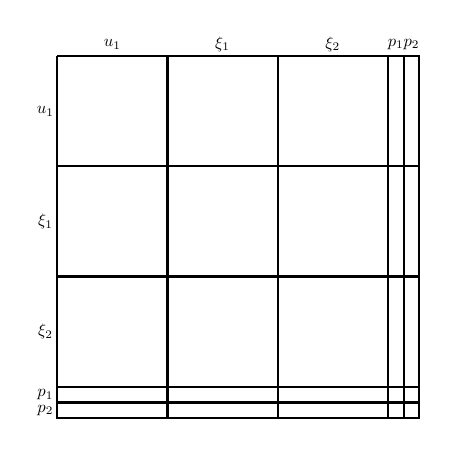
\begin{tikzpicture}[yscale=-1] 

\pgfmathsetmacro{\nt}{7};% time points
\pgfmathsetmacro{\nu}{1}; % controls
\pgfmathsetmacro{\nx}{2}; % states
\pgfmathsetmacro{\np}{2}; % parameters
\pgfmathsetmacro{\nc}{\nu + \nx}; % total continuous

%% control labels
\foreach \k in {1,...,\nu}{
	\pgfmathsetmacro{\x}{0.2*\nt*\k - 0.2/2*(\nt-1)};
	\node () at (\x,-0.05) {\scalebox{0.6}{$u_{\k}$}};
    \node () at (-0.05,\x) {\scalebox{0.6}{$u_{\k}$}};
}

%% state labels
\foreach \k in {1,...,\nx}{
	\pgfmathsetmacro{\x}{0.2*\nt*\k + 0.2*\nu*\nt - 0.2/2*(\nt-1)};
	\node () at (\x,-0.05) {\scalebox{0.6}{$\xi_{\k}$}};
    \node () at (-0.05,\x) {\scalebox{0.6}{$\xi_{\k}$}};
}

%% parameter labels
\foreach \k in {1,...,\np}{
	\pgfmathsetmacro{\x}{0.2*\k + 0.2*\nu*\nt + 0.2*\nx*\nt};
	\node () at (\x,-0.05) {\scalebox{0.6}{$p_{\k}$}};
    \node () at (-0.05,\x) {\scalebox{0.6}{$p_{\k}$}};
}


%% controls
\foreach \k in {1,...,\nu}{
	\foreach \j in {1,...,\nu}{
		\foreach \i in {1,...,\nt}{ 
        	\pgfmathsetmacro{\kk}{\k-1};
            \pgfmathsetmacro{\jj}{\j-1};
        	\pgfmathsetmacro{\x}{0.2*\i + 0.2*\kk*\nt};
            \pgfmathsetmacro{\y}{0.2*\i + 0.2*\jj*\nt};
        	\node () at (\x,\y) {\mysparsesymbol};
} 
    \pgfmathsetmacro{\kk}{\k-1};
    \pgfmathsetmacro{\jj}{\j-1};
    \pgfmathsetmacro{\x}{0.2*\kk*\nt + 0.1};
    \pgfmathsetmacro{\y}{0.2*\jj*\nt + 0.1};
	\draw[\mysparseboxcolor,thick](\x,\y) -- (\x+0.2*\nt,\y) -- (\x+0.2*\nt,\y+0.2*\nt) -- (\x,\y+0.2*\nt) -- (\x,\y);
} }

%% states
\foreach \k in {1,...,\nx}{
	\foreach \j in {1,...,\nx}{
		\foreach \i in {1,...,\nt}{ 
        	\pgfmathsetmacro{\kk}{\k-1};
            \pgfmathsetmacro{\jj}{\j-1};
        	\node () at (0.2*\i + 0.2*\kk*\nt + 0.2*\nu*\nt, 0.2*\i + 0.2*\jj*\nt + 0.2*\nu*\nt) {\mysparsesymbol};
} 
    \pgfmathsetmacro{\kk}{\k-1};
    \pgfmathsetmacro{\jj}{\j-1};
    \pgfmathsetmacro{\x}{0.2*\kk*\nt + 0.2*(\nu)*\nt + 0.1};
    \pgfmathsetmacro{\y}{0.2*\jj*\nt + 0.2*(\nu)*\nt + 0.1};
	\draw[\mysparseboxcolor,thick](\x,\y) -- (\x+0.2*\nt,\y) -- (\x+0.2*\nt,\y+0.2*\nt) -- (\x,\y+0.2*\nt) -- (\x,\y);
} }

%% parameters
\foreach \k in {1,...,\np}{
	\foreach \j in {1,...,\np}{
      \pgfmathsetmacro{\kk}{\k-1};
      \pgfmathsetmacro{\jj}{\j-1};
      \node ( ) at (0.2*\j + 0.2*\nx*\nt + 0.2*\nu*\nt, 0.2*\k + 0.2*\nx*\nt + 0.2*\nu*\nt) {\mysparsesymbol};
      \pgfmathsetmacro{\x}{0.2*\kk + 0.2*(\nu)*\nt + 0.2*\nx*\nt + 0.1};
      \pgfmathsetmacro{\y}{0.2*\jj + 0.2*(\nu)*\nt + 0.2*\nx*\nt + 0.1};
      \draw[\mysparseboxcolor,thick](\x,\y) -- (\x+0.2,\y) -- (\x+0.2,\y+0.2) -- (\x,\y+0.2) -- (\x,\y);
} }

%% states and controls
\foreach \k in {1,...,\nu}{
	\foreach \j in {1,...,\nx}{
		\foreach \i in {1,...,\nt}{ 
        	\pgfmathsetmacro{\kk}{\k-1};
            \pgfmathsetmacro{\jj}{\j-1};
        	\node () at ( 0.2*\i + 0.2*\kk*\nt , 0.2*\i + 0.2*\jj*\nt + 0.2*\nu*\nt) {\mysparsesymbol};
        	\node () at ( 0.2*\i + 0.2*\jj*\nt + 0.2*\nu*\nt, 0.2*\i + 0.2*\kk*\nt) {\mysparsesymbol};
} 
    \pgfmathsetmacro{\kk}{\k-1};
    \pgfmathsetmacro{\jj}{\j-1};
    \pgfmathsetmacro{\x}{0.2*\kk*\nt + 0.1};
    \pgfmathsetmacro{\y}{0.2*\jj*\nt + 0.2*(\nu)*\nt + 0.1};
	\draw[\mysparseboxcolor,thick](\x,\y) -- (\x+0.2*\nt,\y) -- (\x+0.2*\nt,\y+0.2*\nt) -- (\x,\y+0.2*\nt) -- (\x,\y);
    \draw[\mysparseboxcolor,thick](\y,\x) -- (\y+0.2*\nt,\x) -- (\y+0.2*\nt,\x+0.2*\nt) -- (\y,\x+0.2*\nt) -- (\y,\x);
} }

%% states and parameters
\foreach \k in {1,...,\np}{
	\foreach \j in {1,...,\nx}{
		\foreach \i in {1,...,\nt}{ 
        	\pgfmathsetmacro{\kk}{\k-1};
            \pgfmathsetmacro{\jj}{\j-1};
        	\node () at ( 0.2*\k + 0.2*\nx*\nt + 0.2*\nu*\nt, 0.2*\i + 0.2*\jj*\nt + 0.2*\nu*\nt ) {\mysparsesymbol};
            \node () at ( 0.2*\i + 0.2*\jj*\nt + 0.2*\nu*\nt, 0.2*\k + 0.2*\nx*\nt + 0.2*\nu*\nt ) {\mysparsesymbol};
} 
    \pgfmathsetmacro{\kk}{\k-1};
    \pgfmathsetmacro{\jj}{\j-1};
    \pgfmathsetmacro{\x}{0.2*\kk + 0.2*\nx*\nt + 0.2*\nu*\nt + 0.1};
    \pgfmathsetmacro{\y}{0.2*\jj*\nt + 0.2*\nu*\nt + 0.1};
	\draw[\mysparseboxcolor,thick](\x,\y) -- (\x+0.2,\y) -- (\x+0.2,\y+0.2*\nt) -- (\x,\y+0.2*\nt) -- (\x,\y);
    \draw[\mysparseboxcolor,thick](\y,\x) -- (\y+0.2*\nt,\x) -- (\y+0.2*\nt,\x+0.2) -- (\y,\x+0.2) -- (\y,\x);

} }

%% controls and parameters
\foreach \k in {1,...,\np}{
	\foreach \j in {1,...,\nu}{
		\foreach \i in {1,...,\nt}{ 
        	\pgfmathsetmacro{\kk}{\k-1};
            \pgfmathsetmacro{\jj}{\j-1};
        	\node () at ( 0.2*\k + 0.2*\nx*\nt + 0.2*\nu*\nt, 0.2*\i + 0.2*\jj*\nt ) {\mysparsesymbol};
            \node () at ( 0.2*\i + 0.2*\jj*\nt , 0.2*\k + 0.2*\nx*\nt + 0.2*\nu*\nt ) {\mysparsesymbol};
} 
    \pgfmathsetmacro{\kk}{\k-1};
    \pgfmathsetmacro{\jj}{\j-1};
    \pgfmathsetmacro{\x}{0.2*\kk + 0.2*\nx*\nt + 0.2*\nu*\nt + 0.1};
    \pgfmathsetmacro{\y}{0.2*\jj*\nt + 0.1};
	\draw[\mysparseboxcolor,thick](\x,\y) -- (\x+0.2,\y) -- (\x+0.2,\y+0.2*\nt) -- (\x,\y+0.2*\nt) -- (\x,\y);
    \draw[\mysparseboxcolor,thick](\y,\x) -- (\y+0.2*\nt,\x) -- (\y+0.2*\nt,\x+0.2) -- (\y,\x+0.2) -- (\y,\x);
} }

%% initial states
\foreach \k in {1,...,\nx}{
	\foreach \j in {1,...,\nc}{
		\foreach \i in {1,...,\nt}{ 
        	\pgfmathsetmacro{\kk}{\k-1};
            \pgfmathsetmacro{\jj}{\j-1};
        	\node () at (0.2 + 0.2*\kk*\nt + 0.2*\nu*\nt, 0.2*\i + 0.2*\jj*\nt ) {\mysparsesymbol};
            \node () at ( 0.2*\i + 0.2*\jj*\nt , 0.2 + 0.2*\kk*\nt + 0.2*\nu*\nt ) {\mysparsesymbol};
} } 
	\foreach \j in {1,...,\np}{
		\pgfmathsetmacro{\kk}{\k-1};
        \pgfmathsetmacro{\jj}{\j-1};
        \node () at ( 0.2*\k + 0.2*\nx*\nt + 0.2*\nu*\nt, 0.2 + 0.2*\jj*\nt + 0.2*\nu*\nt ) {\mysparsesymbol};
        \node () at ( 0.2 + 0.2*\jj*\nt + 0.2*\nu*\nt , 0.2*\k + 0.2*\nx*\nt + 0.2*\nu*\nt ) {\mysparsesymbol};
	}
}

%% final states
\foreach \k in {1,...,\nx}{
	\foreach \j in {1,...,\nc}{
		\foreach \i in {1,...,\nt}{ 
        	\pgfmathsetmacro{\kk}{\k-1};
            \pgfmathsetmacro{\jj}{\j-1};
        	\node () at (0.2*\nt + 0.2*\kk*\nt + 0.2*\nu*\nt, 0.2*\i + 0.2*\jj*\nt ) {\mysparsesymbol};
            \node () at ( 0.2*\i + 0.2*\jj*\nt , 0.2*\nt + 0.2*\kk*\nt + 0.2*\nu*\nt ) {\mysparsesymbol};
} } 
	\foreach \j in {1,...,\np}{
		\pgfmathsetmacro{\kk}{\k-1};
        \pgfmathsetmacro{\jj}{\j-1};
        \node () at ( 0.2*\k + 0.2*\nx*\nt + 0.2*\nu*\nt, 0.2*\nt + 0.2*\jj*\nt + 0.2*\nu*\nt ) {\mysparsesymbol};
        \node () at ( 0.2*\nt + 0.2*\jj*\nt + 0.2*\nu*\nt , 0.2*\k + 0.2*\nx*\nt + 0.2*\nu*\nt ) {\mysparsesymbol};
	}
}


























% %% states and controls
% \foreach \k in {0,...,2}{
% 	\foreach \j in {0,...,2}{
% 		\foreach \i in {1,...,5}{ 
%         	\node () at (0.2*\i + \k,0.2*\i + \j) {\mysparsesymbol};
% } } }

% %% parameters - right
% \foreach \k in {0,...,1}{
% 	\foreach \j in {0,...,2}{
% 		\foreach \i in {1,...,5}{
%         	\node ( ) at (0.2*\k + 3.2, 0.2*\i + \j) {\mysparsesymbol};
% } } }

% %% parameters - bottom
% \foreach \k in {0,...,1}{
% 	\foreach \j in {0,...,2}{
% 		\foreach \i in {1,...,5}{
%         	\node ( ) at (0.2*\i + \j, 0.2*\k + 3.2) {\mysparsesymbol};
% } } }

% %% parameters - corner
% \foreach \k in {0,...,1}{
% 	\foreach \j in {0,...,1}{
%         	\node ( ) at (0.2*\j + 3.2, 0.2*\k + 3.2) {\mysparsesymbol};
% } }

% %% initial states - bottom
% \foreach \k in {0,...,1}{
% 	\foreach \j in {0,...,2}{
% 		\foreach \i in {1,...,5}{
%         	\node ( ) at (0.2*\i + \j, \k + 1.2) {\mysparsesymbol};
% } } }

% %% final states - bottom
% \foreach \k in {0,...,1}{
% 	\foreach \j in {0,...,2}{
% 		\foreach \i in {1,...,5}{
%         	\node ( ) at (0.2*\i + \j, \k + 2.0) {\mysparsesymbol};
% } } }

% %% initial states - right
% \foreach \k in {0,...,1}{
% 	\foreach \j in {0,...,2}{
% 		\foreach \i in {1,...,5}{
%         	\node ( ) at (\k + 1.2, 0.2*\i + \j) {\mysparsesymbol};
% } } }

% %% final states - right
% \foreach \k in {0,...,1}{
% 	\foreach \j in {0,...,2}{
% 		\foreach \i in {1,...,5}{
%         	\node ( ) at (\k + 2.0, 0.2*\i + \j) {\mysparsesymbol};
% } } }


% %% draw boxes - states and controls
% \foreach \k in {0,...,2}{
% 	\foreach \j in {0,...,2}{
%     	\pgfmathsetmacro{\x}{\k + 0.1};
%     	\pgfmathsetmacro{\y}{\j + 0.1};
%         \draw[blue!70] (\x,\y) -- (\x+1,\y) -- (\x+1,\y+1) -- (\x,\y+1) -- (\x,\y);
% } }

% %% draw boxes - parameters - right
% \foreach \k in {0,...,1}{
% 	\foreach \j in {0,...,2}{
%     	\pgfmathsetmacro{\x}{0.2*\k + 0.1 + 3};
%     	\pgfmathsetmacro{\y}{\j + 0.1};
%         \draw[blue] (\x,\y) -- (\x+0.2,\y) -- (\x+0.2,\y+1) -- (\x,\y+1) -- (\x,\y);
% } }

% %% draw boxes - parameters - bottom
% \foreach \k in {0,...,2}{
% 	\foreach \j in {0,...,1}{
%     	\pgfmathsetmacro{\x}{\k + 0.1};
%     	\pgfmathsetmacro{\y}{0.2*\j + 0.1 + 3};
%         \draw[blue] (\x,\y) -- (\x+1,\y) -- (\x+1,\y+0.2) -- (\x,\y+0.2) -- (\x,\y);
% } }

% %% draw boxes - parameters - bottom
% \foreach \k in {0,...,1}{
% 	\foreach \j in {0,...,1}{
%     	\pgfmathsetmacro{\x}{0.2*\k + 0.1 + 3};
%     	\pgfmathsetmacro{\y}{0.2*\j + 0.1 + 3};
%         \draw[blue] (\x,\y) -- (\x+0.2,\y) -- (\x+0.2,\y+0.2) -- (\x,\y+0.2) -- (\x,\y);
% } }


%% final states
\foreach \k in {1,...,\nx}{
	\foreach \j in {1,...,\nc}{
		\foreach \i in {1,...,\nt}{ 
        	\pgfmathsetmacro{\kk}{\k-1};
            \pgfmathsetmacro{\jj}{\j-1};
        	\node () at (0.2*\nt + 0.2*\kk*\nt + 0.2*\nu*\nt, 0.2*\i + 0.2*\jj*\nt ) {\mytemp};
            \node () at ( 0.2*\i + 0.2*\jj*\nt , 0.2*\nt + 0.2*\kk*\nt + 0.2*\nu*\nt ) {\mytemp};
} } 
	\foreach \j in {1,...,\np}{
		\pgfmathsetmacro{\kk}{\k-1};
        \pgfmathsetmacro{\jj}{\j-1};
        \node () at ( 0.2*\k + 0.2*\nx*\nt + 0.2*\nu*\nt, 0.2*\nt + 0.2*\jj*\nt + 0.2*\nu*\nt ) {\mytemp};
        \node () at ( 0.2*\nt + 0.2*\jj*\nt + 0.2*\nu*\nt , 0.2*\k + 0.2*\nx*\nt + 0.2*\nu*\nt ) {\mytemp};
	}
}
\end{tikzpicture}
}
% 	\end{minipage}
% }%
% \subfloat[(f) Remaining terms.]{
% 	\begin{minipage}{0.33\textwidth}
% 	\tikzsetnextfilename{Hoff}

\centering
\resizebox{1\textwidth}{!}{
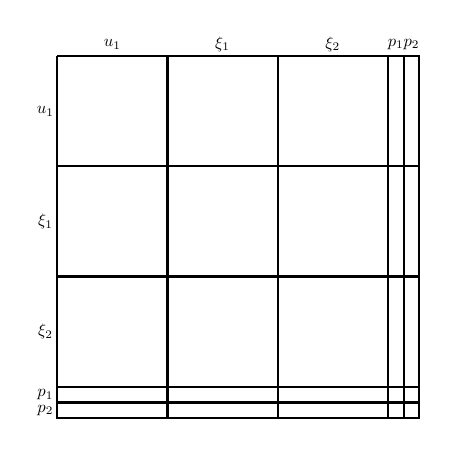
\begin{tikzpicture}[yscale=-1] 

\pgfmathsetmacro{\nt}{7};% time points
\pgfmathsetmacro{\nu}{1}; % controls
\pgfmathsetmacro{\nx}{2}; % states
\pgfmathsetmacro{\np}{2}; % parameters
\pgfmathsetmacro{\nc}{\nu + \nx}; % total continuous

%% control labels
\foreach \k in {1,...,\nu}{
	\pgfmathsetmacro{\x}{0.2*\nt*\k - 0.2/2*(\nt-1)};
	\node () at (\x,-0.05) {\scalebox{0.6}{$u_{\k}$}};
    \node () at (-0.05,\x) {\scalebox{0.6}{$u_{\k}$}};
}

%% state labels
\foreach \k in {1,...,\nx}{
	\pgfmathsetmacro{\x}{0.2*\nt*\k + 0.2*\nu*\nt - 0.2/2*(\nt-1)};
	\node () at (\x,-0.05) {\scalebox{0.6}{$\xi_{\k}$}};
    \node () at (-0.05,\x) {\scalebox{0.6}{$\xi_{\k}$}};
}

%% parameter labels
\foreach \k in {1,...,\np}{
	\pgfmathsetmacro{\x}{0.2*\k + 0.2*\nu*\nt + 0.2*\nx*\nt};
	\node () at (\x,-0.05) {\scalebox{0.6}{$p_{\k}$}};
    \node () at (-0.05,\x) {\scalebox{0.6}{$p_{\k}$}};
}


%% controls
\foreach \k in {1,...,\nu}{
	\foreach \j in {1,...,\nu}{
		\foreach \i in {1,...,\nt}{ 
        	\pgfmathsetmacro{\kk}{\k-1};
            \pgfmathsetmacro{\jj}{\j-1};
        	\pgfmathsetmacro{\x}{0.2*\i + 0.2*\kk*\nt};
            \pgfmathsetmacro{\y}{0.2*\i + 0.2*\jj*\nt};
        	\node () at (\x,\y) {\mysparsesymbol};
} 
    \pgfmathsetmacro{\kk}{\k-1};
    \pgfmathsetmacro{\jj}{\j-1};
    \pgfmathsetmacro{\x}{0.2*\kk*\nt + 0.1};
    \pgfmathsetmacro{\y}{0.2*\jj*\nt + 0.1};
	\draw[\mysparseboxcolor,thick](\x,\y) -- (\x+0.2*\nt,\y) -- (\x+0.2*\nt,\y+0.2*\nt) -- (\x,\y+0.2*\nt) -- (\x,\y);
} }

%% states
\foreach \k in {1,...,\nx}{
	\foreach \j in {1,...,\nx}{
		\foreach \i in {1,...,\nt}{ 
        	\pgfmathsetmacro{\kk}{\k-1};
            \pgfmathsetmacro{\jj}{\j-1};
        	\node () at (0.2*\i + 0.2*\kk*\nt + 0.2*\nu*\nt, 0.2*\i + 0.2*\jj*\nt + 0.2*\nu*\nt) {\mysparsesymbol};
} 
    \pgfmathsetmacro{\kk}{\k-1};
    \pgfmathsetmacro{\jj}{\j-1};
    \pgfmathsetmacro{\x}{0.2*\kk*\nt + 0.2*(\nu)*\nt + 0.1};
    \pgfmathsetmacro{\y}{0.2*\jj*\nt + 0.2*(\nu)*\nt + 0.1};
	\draw[\mysparseboxcolor,thick](\x,\y) -- (\x+0.2*\nt,\y) -- (\x+0.2*\nt,\y+0.2*\nt) -- (\x,\y+0.2*\nt) -- (\x,\y);
} }

%% parameters
\foreach \k in {1,...,\np}{
	\foreach \j in {1,...,\np}{
      \pgfmathsetmacro{\kk}{\k-1};
      \pgfmathsetmacro{\jj}{\j-1};
      \node ( ) at (0.2*\j + 0.2*\nx*\nt + 0.2*\nu*\nt, 0.2*\k + 0.2*\nx*\nt + 0.2*\nu*\nt) {\mysparsesymbol};
      \pgfmathsetmacro{\x}{0.2*\kk + 0.2*(\nu)*\nt + 0.2*\nx*\nt + 0.1};
      \pgfmathsetmacro{\y}{0.2*\jj + 0.2*(\nu)*\nt + 0.2*\nx*\nt + 0.1};
      \draw[\mysparseboxcolor,thick](\x,\y) -- (\x+0.2,\y) -- (\x+0.2,\y+0.2) -- (\x,\y+0.2) -- (\x,\y);
} }

%% states and controls
\foreach \k in {1,...,\nu}{
	\foreach \j in {1,...,\nx}{
		\foreach \i in {1,...,\nt}{ 
        	\pgfmathsetmacro{\kk}{\k-1};
            \pgfmathsetmacro{\jj}{\j-1};
        	\node () at ( 0.2*\i + 0.2*\kk*\nt , 0.2*\i + 0.2*\jj*\nt + 0.2*\nu*\nt) {\mysparsesymbol};
        	\node () at ( 0.2*\i + 0.2*\jj*\nt + 0.2*\nu*\nt, 0.2*\i + 0.2*\kk*\nt) {\mysparsesymbol};
} 
    \pgfmathsetmacro{\kk}{\k-1};
    \pgfmathsetmacro{\jj}{\j-1};
    \pgfmathsetmacro{\x}{0.2*\kk*\nt + 0.1};
    \pgfmathsetmacro{\y}{0.2*\jj*\nt + 0.2*(\nu)*\nt + 0.1};
	\draw[\mysparseboxcolor,thick](\x,\y) -- (\x+0.2*\nt,\y) -- (\x+0.2*\nt,\y+0.2*\nt) -- (\x,\y+0.2*\nt) -- (\x,\y);
    \draw[\mysparseboxcolor,thick](\y,\x) -- (\y+0.2*\nt,\x) -- (\y+0.2*\nt,\x+0.2*\nt) -- (\y,\x+0.2*\nt) -- (\y,\x);
} }

%% states and parameters
\foreach \k in {1,...,\np}{
	\foreach \j in {1,...,\nx}{
		\foreach \i in {1,...,\nt}{ 
        	\pgfmathsetmacro{\kk}{\k-1};
            \pgfmathsetmacro{\jj}{\j-1};
        	\node () at ( 0.2*\k + 0.2*\nx*\nt + 0.2*\nu*\nt, 0.2*\i + 0.2*\jj*\nt + 0.2*\nu*\nt ) {\mysparsesymbol};
            \node () at ( 0.2*\i + 0.2*\jj*\nt + 0.2*\nu*\nt, 0.2*\k + 0.2*\nx*\nt + 0.2*\nu*\nt ) {\mysparsesymbol};
} 
    \pgfmathsetmacro{\kk}{\k-1};
    \pgfmathsetmacro{\jj}{\j-1};
    \pgfmathsetmacro{\x}{0.2*\kk + 0.2*\nx*\nt + 0.2*\nu*\nt + 0.1};
    \pgfmathsetmacro{\y}{0.2*\jj*\nt + 0.2*\nu*\nt + 0.1};
	\draw[\mysparseboxcolor,thick](\x,\y) -- (\x+0.2,\y) -- (\x+0.2,\y+0.2*\nt) -- (\x,\y+0.2*\nt) -- (\x,\y);
    \draw[\mysparseboxcolor,thick](\y,\x) -- (\y+0.2*\nt,\x) -- (\y+0.2*\nt,\x+0.2) -- (\y,\x+0.2) -- (\y,\x);

} }

%% controls and parameters
\foreach \k in {1,...,\np}{
	\foreach \j in {1,...,\nu}{
		\foreach \i in {1,...,\nt}{ 
        	\pgfmathsetmacro{\kk}{\k-1};
            \pgfmathsetmacro{\jj}{\j-1};
        	\node () at ( 0.2*\k + 0.2*\nx*\nt + 0.2*\nu*\nt, 0.2*\i + 0.2*\jj*\nt ) {\mysparsesymbol};
            \node () at ( 0.2*\i + 0.2*\jj*\nt , 0.2*\k + 0.2*\nx*\nt + 0.2*\nu*\nt ) {\mysparsesymbol};
} 
    \pgfmathsetmacro{\kk}{\k-1};
    \pgfmathsetmacro{\jj}{\j-1};
    \pgfmathsetmacro{\x}{0.2*\kk + 0.2*\nx*\nt + 0.2*\nu*\nt + 0.1};
    \pgfmathsetmacro{\y}{0.2*\jj*\nt + 0.1};
	\draw[\mysparseboxcolor,thick](\x,\y) -- (\x+0.2,\y) -- (\x+0.2,\y+0.2*\nt) -- (\x,\y+0.2*\nt) -- (\x,\y);
    \draw[\mysparseboxcolor,thick](\y,\x) -- (\y+0.2*\nt,\x) -- (\y+0.2*\nt,\x+0.2) -- (\y,\x+0.2) -- (\y,\x);
} }

%% initial states
\foreach \k in {1,...,\nx}{
	\foreach \j in {1,...,\nc}{
		\foreach \i in {1,...,\nt}{ 
        	\pgfmathsetmacro{\kk}{\k-1};
            \pgfmathsetmacro{\jj}{\j-1};
        	\node () at (0.2 + 0.2*\kk*\nt + 0.2*\nu*\nt, 0.2*\i + 0.2*\jj*\nt ) {\mysparsesymbol};
            \node () at ( 0.2*\i + 0.2*\jj*\nt , 0.2 + 0.2*\kk*\nt + 0.2*\nu*\nt ) {\mysparsesymbol};
} } 
	\foreach \j in {1,...,\np}{
		\pgfmathsetmacro{\kk}{\k-1};
        \pgfmathsetmacro{\jj}{\j-1};
        \node () at ( 0.2*\k + 0.2*\nx*\nt + 0.2*\nu*\nt, 0.2 + 0.2*\jj*\nt + 0.2*\nu*\nt ) {\mysparsesymbol};
        \node () at ( 0.2 + 0.2*\jj*\nt + 0.2*\nu*\nt , 0.2*\k + 0.2*\nx*\nt + 0.2*\nu*\nt ) {\mysparsesymbol};
	}
}

%% final states
\foreach \k in {1,...,\nx}{
	\foreach \j in {1,...,\nc}{
		\foreach \i in {1,...,\nt}{ 
        	\pgfmathsetmacro{\kk}{\k-1};
            \pgfmathsetmacro{\jj}{\j-1};
        	\node () at (0.2*\nt + 0.2*\kk*\nt + 0.2*\nu*\nt, 0.2*\i + 0.2*\jj*\nt ) {\mysparsesymbol};
            \node () at ( 0.2*\i + 0.2*\jj*\nt , 0.2*\nt + 0.2*\kk*\nt + 0.2*\nu*\nt ) {\mysparsesymbol};
} } 
	\foreach \j in {1,...,\np}{
		\pgfmathsetmacro{\kk}{\k-1};
        \pgfmathsetmacro{\jj}{\j-1};
        \node () at ( 0.2*\k + 0.2*\nx*\nt + 0.2*\nu*\nt, 0.2*\nt + 0.2*\jj*\nt + 0.2*\nu*\nt ) {\mysparsesymbol};
        \node () at ( 0.2*\nt + 0.2*\jj*\nt + 0.2*\nu*\nt , 0.2*\k + 0.2*\nx*\nt + 0.2*\nu*\nt ) {\mysparsesymbol};
	}
}


























% %% states and controls
% \foreach \k in {0,...,2}{
% 	\foreach \j in {0,...,2}{
% 		\foreach \i in {1,...,5}{ 
%         	\node () at (0.2*\i + \k,0.2*\i + \j) {\mysparsesymbol};
% } } }

% %% parameters - right
% \foreach \k in {0,...,1}{
% 	\foreach \j in {0,...,2}{
% 		\foreach \i in {1,...,5}{
%         	\node ( ) at (0.2*\k + 3.2, 0.2*\i + \j) {\mysparsesymbol};
% } } }

% %% parameters - bottom
% \foreach \k in {0,...,1}{
% 	\foreach \j in {0,...,2}{
% 		\foreach \i in {1,...,5}{
%         	\node ( ) at (0.2*\i + \j, 0.2*\k + 3.2) {\mysparsesymbol};
% } } }

% %% parameters - corner
% \foreach \k in {0,...,1}{
% 	\foreach \j in {0,...,1}{
%         	\node ( ) at (0.2*\j + 3.2, 0.2*\k + 3.2) {\mysparsesymbol};
% } }

% %% initial states - bottom
% \foreach \k in {0,...,1}{
% 	\foreach \j in {0,...,2}{
% 		\foreach \i in {1,...,5}{
%         	\node ( ) at (0.2*\i + \j, \k + 1.2) {\mysparsesymbol};
% } } }

% %% final states - bottom
% \foreach \k in {0,...,1}{
% 	\foreach \j in {0,...,2}{
% 		\foreach \i in {1,...,5}{
%         	\node ( ) at (0.2*\i + \j, \k + 2.0) {\mysparsesymbol};
% } } }

% %% initial states - right
% \foreach \k in {0,...,1}{
% 	\foreach \j in {0,...,2}{
% 		\foreach \i in {1,...,5}{
%         	\node ( ) at (\k + 1.2, 0.2*\i + \j) {\mysparsesymbol};
% } } }

% %% final states - right
% \foreach \k in {0,...,1}{
% 	\foreach \j in {0,...,2}{
% 		\foreach \i in {1,...,5}{
%         	\node ( ) at (\k + 2.0, 0.2*\i + \j) {\mysparsesymbol};
% } } }


% %% draw boxes - states and controls
% \foreach \k in {0,...,2}{
% 	\foreach \j in {0,...,2}{
%     	\pgfmathsetmacro{\x}{\k + 0.1};
%     	\pgfmathsetmacro{\y}{\j + 0.1};
%         \draw[blue!70] (\x,\y) -- (\x+1,\y) -- (\x+1,\y+1) -- (\x,\y+1) -- (\x,\y);
% } }

% %% draw boxes - parameters - right
% \foreach \k in {0,...,1}{
% 	\foreach \j in {0,...,2}{
%     	\pgfmathsetmacro{\x}{0.2*\k + 0.1 + 3};
%     	\pgfmathsetmacro{\y}{\j + 0.1};
%         \draw[blue] (\x,\y) -- (\x+0.2,\y) -- (\x+0.2,\y+1) -- (\x,\y+1) -- (\x,\y);
% } }

% %% draw boxes - parameters - bottom
% \foreach \k in {0,...,2}{
% 	\foreach \j in {0,...,1}{
%     	\pgfmathsetmacro{\x}{\k + 0.1};
%     	\pgfmathsetmacro{\y}{0.2*\j + 0.1 + 3};
%         \draw[blue] (\x,\y) -- (\x+1,\y) -- (\x+1,\y+0.2) -- (\x,\y+0.2) -- (\x,\y);
% } }

% %% draw boxes - parameters - bottom
% \foreach \k in {0,...,1}{
% 	\foreach \j in {0,...,1}{
%     	\pgfmathsetmacro{\x}{0.2*\k + 0.1 + 3};
%     	\pgfmathsetmacro{\y}{0.2*\j + 0.1 + 3};
%         \draw[blue] (\x,\y) -- (\x+0.2,\y) -- (\x+0.2,\y+0.2) -- (\x,\y+0.2) -- (\x,\y);
% } }


%% states and controls
\foreach \k in {1,...,\nu}{
	\foreach \j in {1,...,\nx}{
		\foreach \i in {1,...,\nt}{ 
        	\pgfmathsetmacro{\kk}{\k-1};
            \pgfmathsetmacro{\jj}{\j-1};
        	\node () at ( 0.2*\i + 0.2*\kk*\nt , 0.2*\i + 0.2*\jj*\nt + 0.2*\nu*\nt) {\mytemp};
        	\node () at ( 0.2*\i + 0.2*\jj*\nt + 0.2*\nu*\nt, 0.2*\i + 0.2*\kk*\nt) {\mytemp};
} } }

%% states and parameters
\foreach \k in {1,...,\np}{
	\foreach \j in {1,...,\nx}{
		\foreach \i in {1,...,\nt}{ 
        	\pgfmathsetmacro{\kk}{\k-1};
            \pgfmathsetmacro{\jj}{\j-1};
        	\node () at ( 0.2*\k + 0.2*\nx*\nt + 0.2*\nu*\nt, 0.2*\i + 0.2*\jj*\nt + 0.2*\nu*\nt ) {\mytemp};
            \node () at ( 0.2*\i + 0.2*\jj*\nt + 0.2*\nu*\nt, 0.2*\k + 0.2*\nx*\nt + 0.2*\nu*\nt ) {\mytemp};
} } }

%% controls and parameters
\foreach \k in {1,...,\np}{
	\foreach \j in {1,...,\nu}{
		\foreach \i in {1,...,\nt}{ 
        	\pgfmathsetmacro{\kk}{\k-1};
            \pgfmathsetmacro{\jj}{\j-1};
        	\node () at ( 0.2*\k + 0.2*\nx*\nt + 0.2*\nu*\nt, 0.2*\i + 0.2*\jj*\nt ) {\mytemp};
            \node () at ( 0.2*\i + 0.2*\jj*\nt , 0.2*\k + 0.2*\nx*\nt + 0.2*\nu*\nt ) {\mytemp};
} } }

\end{tikzpicture}
}
% 	\end{minipage}
% }%

% \caption{Sparsity pattern of $\mathbf{H}$ matrix for all considered methods except CQHS.}\label{fig:figsparsityHSS}
% \end{figure}

\begin{figure}[ht]

\centering

\begin{minipage}{0.33\textwidth}
\tikzsetnextfilename{Hcqhs}

\centering
\resizebox{1\textwidth}{!}{
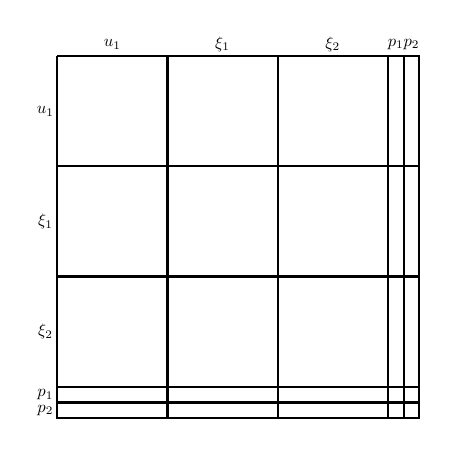
\begin{tikzpicture}[yscale=-1] 

\pgfmathsetmacro{\nt}{7};% time points
\pgfmathsetmacro{\nu}{1}; % controls
\pgfmathsetmacro{\nx}{2}; % states
\pgfmathsetmacro{\np}{2}; % parameters
\pgfmathsetmacro{\nc}{\nu + \nx}; % total continuous

%% control labels
\foreach \k in {1,...,\nu}{
	\pgfmathsetmacro{\x}{0.2*\nt*\k - 0.2/2*(\nt-1)};
	\node () at (\x,-0.05) {\scalebox{0.6}{$u_{\k}$}};
    \node () at (-0.05,\x) {\scalebox{0.6}{$u_{\k}$}};
}

%% state labels
\foreach \k in {1,...,\nx}{
	\pgfmathsetmacro{\x}{0.2*\nt*\k + 0.2*\nu*\nt - 0.2/2*(\nt-1)};
	\node () at (\x,-0.05) {\scalebox{0.6}{$\xi_{\k}$}};
    \node () at (-0.05,\x) {\scalebox{0.6}{$\xi_{\k}$}};
}

%% parameter labels
\foreach \k in {1,...,\np}{
	\pgfmathsetmacro{\x}{0.2*\k + 0.2*\nu*\nt + 0.2*\nx*\nt};
	\node () at (\x,-0.05) {\scalebox{0.6}{$p_{\k}$}};
    \node () at (-0.05,\x) {\scalebox{0.6}{$p_{\k}$}};
}


%% controls
\foreach \k in {1,...,\nu}{
	\foreach \j in {1,...,\nu}{
		\foreach \i in {1,...,\nt}{ 
        	\pgfmathsetmacro{\kk}{\k-1};
            \pgfmathsetmacro{\jj}{\j-1};
        	\pgfmathsetmacro{\x}{0.2*\i + 0.2*\kk*\nt};
            \pgfmathsetmacro{\y}{0.2*\i + 0.2*\jj*\nt};
        	\node () at (\x,\y) {\mysparsesymbol};
} 
    \pgfmathsetmacro{\kk}{\k-1};
    \pgfmathsetmacro{\jj}{\j-1};
    \pgfmathsetmacro{\x}{0.2*\kk*\nt + 0.1};
    \pgfmathsetmacro{\y}{0.2*\jj*\nt + 0.1};
	\draw[\mysparseboxcolor,thick](\x,\y) -- (\x+0.2*\nt,\y) -- (\x+0.2*\nt,\y+0.2*\nt) -- (\x,\y+0.2*\nt) -- (\x,\y);
} }

%% states
\foreach \k in {1,...,\nx}{
	\foreach \j in {1,...,\nx}{
		\foreach \i in {1,...,\nt}{ 
        	\pgfmathsetmacro{\kk}{\k-1};
            \pgfmathsetmacro{\jj}{\j-1};
        	\node () at (0.2*\i + 0.2*\kk*\nt + 0.2*\nu*\nt, 0.2*\i + 0.2*\jj*\nt + 0.2*\nu*\nt) {\mysparsesymbol};
} 
    \pgfmathsetmacro{\kk}{\k-1};
    \pgfmathsetmacro{\jj}{\j-1};
    \pgfmathsetmacro{\x}{0.2*\kk*\nt + 0.2*(\nu)*\nt + 0.1};
    \pgfmathsetmacro{\y}{0.2*\jj*\nt + 0.2*(\nu)*\nt + 0.1};
	\draw[\mysparseboxcolor,thick](\x,\y) -- (\x+0.2*\nt,\y) -- (\x+0.2*\nt,\y+0.2*\nt) -- (\x,\y+0.2*\nt) -- (\x,\y);
} }

%% parameters
\foreach \k in {1,...,\np}{
	\foreach \j in {1,...,\np}{
      \pgfmathsetmacro{\kk}{\k-1};
      \pgfmathsetmacro{\jj}{\j-1};
      \node ( ) at (0.2*\j + 0.2*\nx*\nt + 0.2*\nu*\nt, 0.2*\k + 0.2*\nx*\nt + 0.2*\nu*\nt) {\mysparsesymbol};
      \pgfmathsetmacro{\x}{0.2*\kk + 0.2*(\nu)*\nt + 0.2*\nx*\nt + 0.1};
      \pgfmathsetmacro{\y}{0.2*\jj + 0.2*(\nu)*\nt + 0.2*\nx*\nt + 0.1};
      \draw[\mysparseboxcolor,thick](\x,\y) -- (\x+0.2,\y) -- (\x+0.2,\y+0.2) -- (\x,\y+0.2) -- (\x,\y);
} }

%% states and controls
\foreach \k in {1,...,\nu}{
	\foreach \j in {1,...,\nx}{
		\foreach \i in {1,...,\nt}{ 
        	\pgfmathsetmacro{\kk}{\k-1};
            \pgfmathsetmacro{\jj}{\j-1};
        	\node () at ( 0.2*\i + 0.2*\kk*\nt , 0.2*\i + 0.2*\jj*\nt + 0.2*\nu*\nt) {\mysparsesymbol};
        	\node () at ( 0.2*\i + 0.2*\jj*\nt + 0.2*\nu*\nt, 0.2*\i + 0.2*\kk*\nt) {\mysparsesymbol};
} 
    \pgfmathsetmacro{\kk}{\k-1};
    \pgfmathsetmacro{\jj}{\j-1};
    \pgfmathsetmacro{\x}{0.2*\kk*\nt + 0.1};
    \pgfmathsetmacro{\y}{0.2*\jj*\nt + 0.2*(\nu)*\nt + 0.1};
	\draw[\mysparseboxcolor,thick](\x,\y) -- (\x+0.2*\nt,\y) -- (\x+0.2*\nt,\y+0.2*\nt) -- (\x,\y+0.2*\nt) -- (\x,\y);
    \draw[\mysparseboxcolor,thick](\y,\x) -- (\y+0.2*\nt,\x) -- (\y+0.2*\nt,\x+0.2*\nt) -- (\y,\x+0.2*\nt) -- (\y,\x);
} }

%% states and parameters
\foreach \k in {1,...,\np}{
	\foreach \j in {1,...,\nx}{
		\foreach \i in {1,...,\nt}{ 
        	\pgfmathsetmacro{\kk}{\k-1};
            \pgfmathsetmacro{\jj}{\j-1};
        	\node () at ( 0.2*\k + 0.2*\nx*\nt + 0.2*\nu*\nt, 0.2*\i + 0.2*\jj*\nt + 0.2*\nu*\nt ) {\mysparsesymbol};
            \node () at ( 0.2*\i + 0.2*\jj*\nt + 0.2*\nu*\nt, 0.2*\k + 0.2*\nx*\nt + 0.2*\nu*\nt ) {\mysparsesymbol};
} 
    \pgfmathsetmacro{\kk}{\k-1};
    \pgfmathsetmacro{\jj}{\j-1};
    \pgfmathsetmacro{\x}{0.2*\kk + 0.2*\nx*\nt + 0.2*\nu*\nt + 0.1};
    \pgfmathsetmacro{\y}{0.2*\jj*\nt + 0.2*\nu*\nt + 0.1};
	\draw[\mysparseboxcolor,thick](\x,\y) -- (\x+0.2,\y) -- (\x+0.2,\y+0.2*\nt) -- (\x,\y+0.2*\nt) -- (\x,\y);
    \draw[\mysparseboxcolor,thick](\y,\x) -- (\y+0.2*\nt,\x) -- (\y+0.2*\nt,\x+0.2) -- (\y,\x+0.2) -- (\y,\x);

} }

%% controls and parameters
\foreach \k in {1,...,\np}{
	\foreach \j in {1,...,\nu}{
		\foreach \i in {1,...,\nt}{ 
        	\pgfmathsetmacro{\kk}{\k-1};
            \pgfmathsetmacro{\jj}{\j-1};
        	\node () at ( 0.2*\k + 0.2*\nx*\nt + 0.2*\nu*\nt, 0.2*\i + 0.2*\jj*\nt ) {\mysparsesymbol};
            \node () at ( 0.2*\i + 0.2*\jj*\nt , 0.2*\k + 0.2*\nx*\nt + 0.2*\nu*\nt ) {\mysparsesymbol};
} 
    \pgfmathsetmacro{\kk}{\k-1};
    \pgfmathsetmacro{\jj}{\j-1};
    \pgfmathsetmacro{\x}{0.2*\kk + 0.2*\nx*\nt + 0.2*\nu*\nt + 0.1};
    \pgfmathsetmacro{\y}{0.2*\jj*\nt + 0.1};
	\draw[\mysparseboxcolor,thick](\x,\y) -- (\x+0.2,\y) -- (\x+0.2,\y+0.2*\nt) -- (\x,\y+0.2*\nt) -- (\x,\y);
    \draw[\mysparseboxcolor,thick](\y,\x) -- (\y+0.2*\nt,\x) -- (\y+0.2*\nt,\x+0.2) -- (\y,\x+0.2) -- (\y,\x);
} }

%% initial states
\foreach \k in {1,...,\nx}{
	\foreach \j in {1,...,\nc}{
		\foreach \i in {1,...,\nt}{ 
        	\pgfmathsetmacro{\kk}{\k-1};
            \pgfmathsetmacro{\jj}{\j-1};
        	\node () at (0.2 + 0.2*\kk*\nt + 0.2*\nu*\nt, 0.2*\i + 0.2*\jj*\nt ) {\mysparsesymbol};
            \node () at ( 0.2*\i + 0.2*\jj*\nt , 0.2 + 0.2*\kk*\nt + 0.2*\nu*\nt ) {\mysparsesymbol};
} } 
	\foreach \j in {1,...,\np}{
		\pgfmathsetmacro{\kk}{\k-1};
        \pgfmathsetmacro{\jj}{\j-1};
        \node () at ( 0.2*\k + 0.2*\nx*\nt + 0.2*\nu*\nt, 0.2 + 0.2*\jj*\nt + 0.2*\nu*\nt ) {\mysparsesymbol};
        \node () at ( 0.2 + 0.2*\jj*\nt + 0.2*\nu*\nt , 0.2*\k + 0.2*\nx*\nt + 0.2*\nu*\nt ) {\mysparsesymbol};
	}
}

%% final states
\foreach \k in {1,...,\nx}{
	\foreach \j in {1,...,\nc}{
		\foreach \i in {1,...,\nt}{ 
        	\pgfmathsetmacro{\kk}{\k-1};
            \pgfmathsetmacro{\jj}{\j-1};
        	\node () at (0.2*\nt + 0.2*\kk*\nt + 0.2*\nu*\nt, 0.2*\i + 0.2*\jj*\nt ) {\mysparsesymbol};
            \node () at ( 0.2*\i + 0.2*\jj*\nt , 0.2*\nt + 0.2*\kk*\nt + 0.2*\nu*\nt ) {\mysparsesymbol};
} } 
	\foreach \j in {1,...,\np}{
		\pgfmathsetmacro{\kk}{\k-1};
        \pgfmathsetmacro{\jj}{\j-1};
        \node () at ( 0.2*\k + 0.2*\nx*\nt + 0.2*\nu*\nt, 0.2*\nt + 0.2*\jj*\nt + 0.2*\nu*\nt ) {\mysparsesymbol};
        \node () at ( 0.2*\nt + 0.2*\jj*\nt + 0.2*\nu*\nt , 0.2*\k + 0.2*\nx*\nt + 0.2*\nu*\nt ) {\mysparsesymbol};
	}
}


























% %% states and controls
% \foreach \k in {0,...,2}{
% 	\foreach \j in {0,...,2}{
% 		\foreach \i in {1,...,5}{ 
%         	\node () at (0.2*\i + \k,0.2*\i + \j) {\mysparsesymbol};
% } } }

% %% parameters - right
% \foreach \k in {0,...,1}{
% 	\foreach \j in {0,...,2}{
% 		\foreach \i in {1,...,5}{
%         	\node ( ) at (0.2*\k + 3.2, 0.2*\i + \j) {\mysparsesymbol};
% } } }

% %% parameters - bottom
% \foreach \k in {0,...,1}{
% 	\foreach \j in {0,...,2}{
% 		\foreach \i in {1,...,5}{
%         	\node ( ) at (0.2*\i + \j, 0.2*\k + 3.2) {\mysparsesymbol};
% } } }

% %% parameters - corner
% \foreach \k in {0,...,1}{
% 	\foreach \j in {0,...,1}{
%         	\node ( ) at (0.2*\j + 3.2, 0.2*\k + 3.2) {\mysparsesymbol};
% } }

% %% initial states - bottom
% \foreach \k in {0,...,1}{
% 	\foreach \j in {0,...,2}{
% 		\foreach \i in {1,...,5}{
%         	\node ( ) at (0.2*\i + \j, \k + 1.2) {\mysparsesymbol};
% } } }

% %% final states - bottom
% \foreach \k in {0,...,1}{
% 	\foreach \j in {0,...,2}{
% 		\foreach \i in {1,...,5}{
%         	\node ( ) at (0.2*\i + \j, \k + 2.0) {\mysparsesymbol};
% } } }

% %% initial states - right
% \foreach \k in {0,...,1}{
% 	\foreach \j in {0,...,2}{
% 		\foreach \i in {1,...,5}{
%         	\node ( ) at (\k + 1.2, 0.2*\i + \j) {\mysparsesymbol};
% } } }

% %% final states - right
% \foreach \k in {0,...,1}{
% 	\foreach \j in {0,...,2}{
% 		\foreach \i in {1,...,5}{
%         	\node ( ) at (\k + 2.0, 0.2*\i + \j) {\mysparsesymbol};
% } } }


% %% draw boxes - states and controls
% \foreach \k in {0,...,2}{
% 	\foreach \j in {0,...,2}{
%     	\pgfmathsetmacro{\x}{\k + 0.1};
%     	\pgfmathsetmacro{\y}{\j + 0.1};
%         \draw[blue!70] (\x,\y) -- (\x+1,\y) -- (\x+1,\y+1) -- (\x,\y+1) -- (\x,\y);
% } }

% %% draw boxes - parameters - right
% \foreach \k in {0,...,1}{
% 	\foreach \j in {0,...,2}{
%     	\pgfmathsetmacro{\x}{0.2*\k + 0.1 + 3};
%     	\pgfmathsetmacro{\y}{\j + 0.1};
%         \draw[blue] (\x,\y) -- (\x+0.2,\y) -- (\x+0.2,\y+1) -- (\x,\y+1) -- (\x,\y);
% } }

% %% draw boxes - parameters - bottom
% \foreach \k in {0,...,2}{
% 	\foreach \j in {0,...,1}{
%     	\pgfmathsetmacro{\x}{\k + 0.1};
%     	\pgfmathsetmacro{\y}{0.2*\j + 0.1 + 3};
%         \draw[blue] (\x,\y) -- (\x+1,\y) -- (\x+1,\y+0.2) -- (\x,\y+0.2) -- (\x,\y);
% } }

% %% draw boxes - parameters - bottom
% \foreach \k in {0,...,1}{
% 	\foreach \j in {0,...,1}{
%     	\pgfmathsetmacro{\x}{0.2*\k + 0.1 + 3};
%     	\pgfmathsetmacro{\y}{0.2*\j + 0.1 + 3};
%         \draw[blue] (\x,\y) -- (\x+0.2,\y) -- (\x+0.2,\y+0.2) -- (\x,\y+0.2) -- (\x,\y);
% } }


%% controls
\foreach \k in {1,...,\nu}{
	\foreach \j in {1,...,\nu}{
		\foreach \i in {2,...,\nt}{ 
        	\pgfmathsetmacro{\kk}{\k-1};
            \pgfmathsetmacro{\jj}{\j-1};
            \pgfmathsetmacro{\ii}{\i-1};
        	\node () at (0.2*\ii + 0.2*\kk*\nt + 0.2, 0.2*\ii + 0.2*\jj*\nt ) {\mytemp};
            \node () at ( 0.2*\ii + 0.2*\jj*\nt , 0.2*\ii + 0.2*\kk*\nt + 0.2 ) {\mytemp};
} } }

%% states
\foreach \k in {1,...,\nx}{
	\foreach \j in {1,...,\nx}{
		\foreach \i in {2,...,\nt}{ 
        	\pgfmathsetmacro{\kk}{\k-1};
            \pgfmathsetmacro{\jj}{\j-1};
            \pgfmathsetmacro{\ii}{\i-1};
        	\node () at (0.2*\ii + 0.2*\kk*\nt + 0.2*\nu*\nt + 0.2, 0.2*\ii + 0.2*\jj*\nt + 0.2*\nu*\nt) {\mytemp};
            \node () at ( 0.2*\ii + 0.2*\jj*\nt + 0.2*\nu*\nt , 0.2*\ii + 0.2*\kk*\nt + 0.2*\nu*\nt + 0.2 ) {\mytemp};
} } }


%% states and controls
\foreach \k in {1,...,\nu}{
	\foreach \j in {1,...,\nx}{
		\foreach \i in {2,...,\nt}{ 
        	\pgfmathsetmacro{\kk}{\k-1};
            \pgfmathsetmacro{\jj}{\j-1};
            \pgfmathsetmacro{\ii}{\i-1};
        	\node () at (0.2*\ii + 0.2*\kk*\nt + 0.2, 0.2*\ii + 0.2*\jj*\nt + 0.2*\nu*\nt) {\mytemp};
			\node () at ( 0.2*\ii + 0.2*\jj*\nt + 0.2*\nu*\nt , 0.2*\ii + 0.2*\kk*\nt + 0.2) {\mytemp};
            \node () at (0.2*\ii + 0.2*\kk*\nt , 0.2*\ii + 0.2*\jj*\nt + 0.2*\nu*\nt + 0.2) {\mytemp};
            \node () at ( 0.2*\ii + 0.2*\jj*\nt + 0.2*\nu*\nt + 0.2 , 0.2*\ii + 0.2*\kk*\nt) {\mytemp};
} } }




\end{tikzpicture}
}
\end{minipage}

\caption{Sparsity pattern of the off-diagonal terms of $\{ \bm{L}_{11}, \bm{L}_{12}, \bm{L}_{21}, \bm{L}_{22} \}$ in the $\mathbf{H}$ matrix using the CQHS method.}\label{fig:figsparsityCQHS}
\end{figure}

\begin{figure}[ht]

\centering

\begin{subfigure}{0.33\textwidth}
\centering
\begin{minipage}{1\textwidth}
\input{../ch5/sparsity/Mpp}
\end{minipage}
\caption{$\bm{M}_{33}$ terms.}
% \label{fig:}
\end{subfigure}%
\begin{subfigure}{0.33\textwidth}
\centering
\begin{minipage}{1\textwidth}
\tikzsetnextfilename{Mx0x0}

\centering
\resizebox{1\textwidth}{!}{
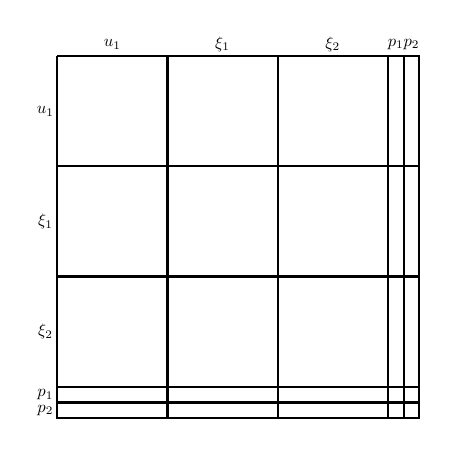
\begin{tikzpicture}[yscale=-1] 

\pgfmathsetmacro{\nt}{7};% time points
\pgfmathsetmacro{\nu}{1}; % controls
\pgfmathsetmacro{\nx}{2}; % states
\pgfmathsetmacro{\np}{2}; % parameters
\pgfmathsetmacro{\nc}{\nu + \nx}; % total continuous

%% control labels
\foreach \k in {1,...,\nu}{
	\pgfmathsetmacro{\x}{0.2*\nt*\k - 0.2/2*(\nt-1)};
	\node () at (\x,-0.05) {\scalebox{0.6}{$u_{\k}$}};
    \node () at (-0.05,\x) {\scalebox{0.6}{$u_{\k}$}};
}

%% state labels
\foreach \k in {1,...,\nx}{
	\pgfmathsetmacro{\x}{0.2*\nt*\k + 0.2*\nu*\nt - 0.2/2*(\nt-1)};
	\node () at (\x,-0.05) {\scalebox{0.6}{$\xi_{\k}$}};
    \node () at (-0.05,\x) {\scalebox{0.6}{$\xi_{\k}$}};
}

%% parameter labels
\foreach \k in {1,...,\np}{
	\pgfmathsetmacro{\x}{0.2*\k + 0.2*\nu*\nt + 0.2*\nx*\nt};
	\node () at (\x,-0.05) {\scalebox{0.6}{$p_{\k}$}};
    \node () at (-0.05,\x) {\scalebox{0.6}{$p_{\k}$}};
}


%% controls
\foreach \k in {1,...,\nu}{
	\foreach \j in {1,...,\nu}{
    \pgfmathsetmacro{\kk}{\k-1};
    \pgfmathsetmacro{\jj}{\j-1};
    \pgfmathsetmacro{\x}{0.2*\kk*\nt + 0.1};
    \pgfmathsetmacro{\y}{0.2*\jj*\nt + 0.1};
	\draw[\mysparseboxcolor,thick](\x,\y) -- (\x+0.2*\nt,\y) -- (\x+0.2*\nt,\y+0.2*\nt) -- (\x,\y+0.2*\nt) -- (\x,\y);
} }

%% states
\foreach \k in {1,...,\nx}{
	\foreach \j in {1,...,\nx}{
    \pgfmathsetmacro{\kk}{\k-1};
    \pgfmathsetmacro{\jj}{\j-1};
    \pgfmathsetmacro{\x}{0.2*\kk*\nt + 0.2*(\nu)*\nt + 0.1};
    \pgfmathsetmacro{\y}{0.2*\jj*\nt + 0.2*(\nu)*\nt + 0.1};
	\draw[\mysparseboxcolor,thick](\x,\y) -- (\x+0.2*\nt,\y) -- (\x+0.2*\nt,\y+0.2*\nt) -- (\x,\y+0.2*\nt) -- (\x,\y);
} }

%% parameters
\foreach \k in {1,...,\np}{
	\foreach \j in {1,...,\np}{
      \pgfmathsetmacro{\kk}{\k-1};
      \pgfmathsetmacro{\jj}{\j-1};
      \pgfmathsetmacro{\x}{0.2*\kk + 0.2*(\nu)*\nt + 0.2*\nx*\nt + 0.1};
      \pgfmathsetmacro{\y}{0.2*\jj + 0.2*(\nu)*\nt + 0.2*\nx*\nt + 0.1};
      \draw[\mysparseboxcolor,thick](\x,\y) -- (\x+0.2,\y) -- (\x+0.2,\y+0.2) -- (\x,\y+0.2) -- (\x,\y);
} }

%% states and controls
\foreach \k in {1,...,\nu}{
	\foreach \j in {1,...,\nx}{ 
    \pgfmathsetmacro{\kk}{\k-1};
    \pgfmathsetmacro{\jj}{\j-1};
    \pgfmathsetmacro{\x}{0.2*\kk*\nt + 0.1};
    \pgfmathsetmacro{\y}{0.2*\jj*\nt + 0.2*(\nu)*\nt + 0.1};
	\draw[\mysparseboxcolor,thick](\x,\y) -- (\x+0.2*\nt,\y) -- (\x+0.2*\nt,\y+0.2*\nt) -- (\x,\y+0.2*\nt) -- (\x,\y);
    \draw[\mysparseboxcolor,thick](\y,\x) -- (\y+0.2*\nt,\x) -- (\y+0.2*\nt,\x+0.2*\nt) -- (\y,\x+0.2*\nt) -- (\y,\x);
} }

%% states and parameters
\foreach \k in {1,...,\np}{
	\foreach \j in {1,...,\nx}{ 
    \pgfmathsetmacro{\kk}{\k-1};
    \pgfmathsetmacro{\jj}{\j-1};
    \pgfmathsetmacro{\x}{0.2*\kk + 0.2*\nx*\nt + 0.2*\nu*\nt + 0.1};
    \pgfmathsetmacro{\y}{0.2*\jj*\nt + 0.2*\nu*\nt + 0.1};
	\draw[\mysparseboxcolor,thick](\x,\y) -- (\x+0.2,\y) -- (\x+0.2,\y+0.2*\nt) -- (\x,\y+0.2*\nt) -- (\x,\y);
    \draw[\mysparseboxcolor,thick](\y,\x) -- (\y+0.2*\nt,\x) -- (\y+0.2*\nt,\x+0.2) -- (\y,\x+0.2) -- (\y,\x);

} }

%% controls and parameters
\foreach \k in {1,...,\np}{
	\foreach \j in {1,...,\nu}{
    \pgfmathsetmacro{\kk}{\k-1};
    \pgfmathsetmacro{\jj}{\j-1};
    \pgfmathsetmacro{\x}{0.2*\kk + 0.2*\nx*\nt + 0.2*\nu*\nt + 0.1};
    \pgfmathsetmacro{\y}{0.2*\jj*\nt + 0.1};
	\draw[\mysparseboxcolor,thick](\x,\y) -- (\x+0.2,\y) -- (\x+0.2,\y+0.2*\nt) -- (\x,\y+0.2*\nt) -- (\x,\y);
    \draw[\mysparseboxcolor,thick](\y,\x) -- (\y+0.2*\nt,\x) -- (\y+0.2*\nt,\x+0.2) -- (\y,\x+0.2) -- (\y,\x);
} }

%% states off 
\foreach \k in {1,...,\nx}{
	\foreach \j in {1,...,\nx}{
      \pgfmathsetmacro{\kk}{\k-1};
      \pgfmathsetmacro{\jj}{\j-1};
      \node () at ( 0.2 + 0.2*\kk*\nt + 0.2*\nu*\nt, 0.2*\nt + 0.2*\jj*\nt + 0.2*\nu*\nt ) {\mysparsesymbol};
      \node () at ( 0.2*\nt + 0.2*\jj*\nt + 0.2*\nu*\nt , 0.2 + 0.2*\kk*\nt + 0.2*\nu*\nt ) {\mysparsesymbol};
} }

%% parameters off
\foreach \k in {1,...,\np}{
	\foreach \j in {1,...,\nx}{
      \pgfmathsetmacro{\kk}{\k-1};
      \pgfmathsetmacro{\jj}{\j-1};
      \node ( ) at (0.2*\nt*\j + 0.2*\nu*\nt, 0.2*\k + 0.2*\nx*\nt + 0.2*\nu*\nt) {\mysparsesymbol};
	  \node ( ) at ( 0.2*\k + 0.2*\nx*\nt + 0.2*\nu*\nt, 0.2*\nt*\j + 0.2*\nu*\nt ) {\mysparsesymbol};
      
      \node ( ) at ( 0.2*\k + 0.2*\nx*\nt + 0.2*\nu*\nt, 0.2*\nt*\j - 0.2*\nt + 0.2 + 0.2*\nu*\nt ) {\mysparsesymbol};
      
      \node ( ) at ( 0.2*\nt*\j - 0.2*\nt + 0.2 + 0.2*\nu*\nt , 0.2*\k + 0.2*\nx*\nt + 0.2*\nu*\nt ) {\mysparsesymbol};
	  
} }

%% parameters
\foreach \k in {1,...,\np}{
      \foreach \j in {1,...,\np}{
      \pgfmathsetmacro{\kk}{\k-1};
      \pgfmathsetmacro{\jj}{\j-1};
      \node ( ) at (0.2*\j + 0.2*\nx*\nt + 0.2*\nu*\nt, 0.2*\k + 0.2*\nx*\nt + 0.2*\nu*\nt) {\mysparsesymbol};
} }

%% initial states
\foreach \k in {1,...,\nx}{
      \foreach \j in {1,...,\nx}{
      \pgfmathsetmacro{\kk}{\k-1};
      \pgfmathsetmacro{\jj}{\j-1};
      \node () at (0.2 + 0.2*\kk*\nt + 0.2*\nu*\nt, 0.2*1 + 0.2*\jj*\nt + 0.2*\nu*\nt ) {\mysparsesymbol};
} }

%% initial states
\foreach \k in {1,...,\nx}{
      \foreach \j in {1,...,\nx}{
      \pgfmathsetmacro{\kk}{\k-1};
      \pgfmathsetmacro{\jj}{\j-1};
      \node () at ( 0.2*\nt + 0.2*\kk*\nt + 0.2*\nu*\nt, 0.2*\nt + 0.2*\jj*\nt + 0.2*\nu*\nt ) {\mysparsesymbol};
} }



%% initial states
\foreach \k in {1,...,\nx}{
	\foreach \j in {1,...,\nx}{
      \pgfmathsetmacro{\kk}{\k-1};
      \pgfmathsetmacro{\jj}{\j-1};
      \node () at (0.2 + 0.2*\kk*\nt + 0.2*\nu*\nt, 0.2*1 + 0.2*\jj*\nt + 0.2*\nu*\nt ) {\mytemp};
} }
   
   
   
  
  
  
  
  
  
\end{tikzpicture}
}
\end{minipage}
\caption{$\bm{M}_{44}$ terms.}
% \label{fig:}
\end{subfigure}%
\begin{subfigure}{0.33\textwidth}
\centering
\begin{minipage}{1\textwidth}
\input{../ch5/sparsity/Mxfxf}
\end{minipage}
\caption{$\bm{M}_{55}$ terms.}
% \label{fig:}
\end{subfigure}%

% \begin{subfigure}{0.33\textwidth}
% \centering
% \begin{minipage}{1\textwidth}
% \tikzsetnextfilename{Moff}

\centering
\resizebox{1\textwidth}{!}{
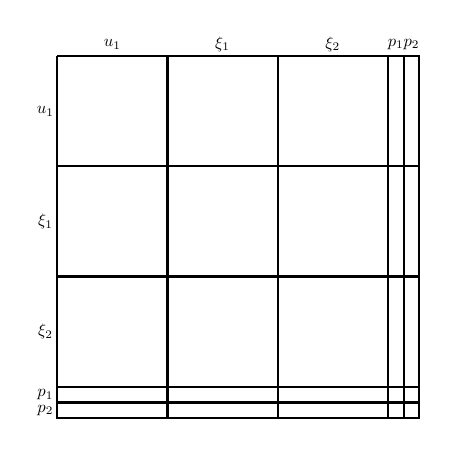
\begin{tikzpicture}[yscale=-1] 

\pgfmathsetmacro{\nt}{7};% time points
\pgfmathsetmacro{\nu}{1}; % controls
\pgfmathsetmacro{\nx}{2}; % states
\pgfmathsetmacro{\np}{2}; % parameters
\pgfmathsetmacro{\nc}{\nu + \nx}; % total continuous

%% control labels
\foreach \k in {1,...,\nu}{
	\pgfmathsetmacro{\x}{0.2*\nt*\k - 0.2/2*(\nt-1)};
	\node () at (\x,-0.05) {\scalebox{0.6}{$u_{\k}$}};
    \node () at (-0.05,\x) {\scalebox{0.6}{$u_{\k}$}};
}

%% state labels
\foreach \k in {1,...,\nx}{
	\pgfmathsetmacro{\x}{0.2*\nt*\k + 0.2*\nu*\nt - 0.2/2*(\nt-1)};
	\node () at (\x,-0.05) {\scalebox{0.6}{$\xi_{\k}$}};
    \node () at (-0.05,\x) {\scalebox{0.6}{$\xi_{\k}$}};
}

%% parameter labels
\foreach \k in {1,...,\np}{
	\pgfmathsetmacro{\x}{0.2*\k + 0.2*\nu*\nt + 0.2*\nx*\nt};
	\node () at (\x,-0.05) {\scalebox{0.6}{$p_{\k}$}};
    \node () at (-0.05,\x) {\scalebox{0.6}{$p_{\k}$}};
}


%% controls
\foreach \k in {1,...,\nu}{
	\foreach \j in {1,...,\nu}{
    \pgfmathsetmacro{\kk}{\k-1};
    \pgfmathsetmacro{\jj}{\j-1};
    \pgfmathsetmacro{\x}{0.2*\kk*\nt + 0.1};
    \pgfmathsetmacro{\y}{0.2*\jj*\nt + 0.1};
	\draw[\mysparseboxcolor,thick](\x,\y) -- (\x+0.2*\nt,\y) -- (\x+0.2*\nt,\y+0.2*\nt) -- (\x,\y+0.2*\nt) -- (\x,\y);
} }

%% states
\foreach \k in {1,...,\nx}{
	\foreach \j in {1,...,\nx}{
    \pgfmathsetmacro{\kk}{\k-1};
    \pgfmathsetmacro{\jj}{\j-1};
    \pgfmathsetmacro{\x}{0.2*\kk*\nt + 0.2*(\nu)*\nt + 0.1};
    \pgfmathsetmacro{\y}{0.2*\jj*\nt + 0.2*(\nu)*\nt + 0.1};
	\draw[\mysparseboxcolor,thick](\x,\y) -- (\x+0.2*\nt,\y) -- (\x+0.2*\nt,\y+0.2*\nt) -- (\x,\y+0.2*\nt) -- (\x,\y);
} }

%% parameters
\foreach \k in {1,...,\np}{
	\foreach \j in {1,...,\np}{
      \pgfmathsetmacro{\kk}{\k-1};
      \pgfmathsetmacro{\jj}{\j-1};
      \pgfmathsetmacro{\x}{0.2*\kk + 0.2*(\nu)*\nt + 0.2*\nx*\nt + 0.1};
      \pgfmathsetmacro{\y}{0.2*\jj + 0.2*(\nu)*\nt + 0.2*\nx*\nt + 0.1};
      \draw[\mysparseboxcolor,thick](\x,\y) -- (\x+0.2,\y) -- (\x+0.2,\y+0.2) -- (\x,\y+0.2) -- (\x,\y);
} }

%% states and controls
\foreach \k in {1,...,\nu}{
	\foreach \j in {1,...,\nx}{ 
    \pgfmathsetmacro{\kk}{\k-1};
    \pgfmathsetmacro{\jj}{\j-1};
    \pgfmathsetmacro{\x}{0.2*\kk*\nt + 0.1};
    \pgfmathsetmacro{\y}{0.2*\jj*\nt + 0.2*(\nu)*\nt + 0.1};
	\draw[\mysparseboxcolor,thick](\x,\y) -- (\x+0.2*\nt,\y) -- (\x+0.2*\nt,\y+0.2*\nt) -- (\x,\y+0.2*\nt) -- (\x,\y);
    \draw[\mysparseboxcolor,thick](\y,\x) -- (\y+0.2*\nt,\x) -- (\y+0.2*\nt,\x+0.2*\nt) -- (\y,\x+0.2*\nt) -- (\y,\x);
} }

%% states and parameters
\foreach \k in {1,...,\np}{
	\foreach \j in {1,...,\nx}{ 
    \pgfmathsetmacro{\kk}{\k-1};
    \pgfmathsetmacro{\jj}{\j-1};
    \pgfmathsetmacro{\x}{0.2*\kk + 0.2*\nx*\nt + 0.2*\nu*\nt + 0.1};
    \pgfmathsetmacro{\y}{0.2*\jj*\nt + 0.2*\nu*\nt + 0.1};
	\draw[\mysparseboxcolor,thick](\x,\y) -- (\x+0.2,\y) -- (\x+0.2,\y+0.2*\nt) -- (\x,\y+0.2*\nt) -- (\x,\y);
    \draw[\mysparseboxcolor,thick](\y,\x) -- (\y+0.2*\nt,\x) -- (\y+0.2*\nt,\x+0.2) -- (\y,\x+0.2) -- (\y,\x);

} }

%% controls and parameters
\foreach \k in {1,...,\np}{
	\foreach \j in {1,...,\nu}{
    \pgfmathsetmacro{\kk}{\k-1};
    \pgfmathsetmacro{\jj}{\j-1};
    \pgfmathsetmacro{\x}{0.2*\kk + 0.2*\nx*\nt + 0.2*\nu*\nt + 0.1};
    \pgfmathsetmacro{\y}{0.2*\jj*\nt + 0.1};
	\draw[\mysparseboxcolor,thick](\x,\y) -- (\x+0.2,\y) -- (\x+0.2,\y+0.2*\nt) -- (\x,\y+0.2*\nt) -- (\x,\y);
    \draw[\mysparseboxcolor,thick](\y,\x) -- (\y+0.2*\nt,\x) -- (\y+0.2*\nt,\x+0.2) -- (\y,\x+0.2) -- (\y,\x);
} }

%% states off 
\foreach \k in {1,...,\nx}{
	\foreach \j in {1,...,\nx}{
      \pgfmathsetmacro{\kk}{\k-1};
      \pgfmathsetmacro{\jj}{\j-1};
      \node () at ( 0.2 + 0.2*\kk*\nt + 0.2*\nu*\nt, 0.2*\nt + 0.2*\jj*\nt + 0.2*\nu*\nt ) {\mysparsesymbol};
      \node () at ( 0.2*\nt + 0.2*\jj*\nt + 0.2*\nu*\nt , 0.2 + 0.2*\kk*\nt + 0.2*\nu*\nt ) {\mysparsesymbol};
} }

%% parameters off
\foreach \k in {1,...,\np}{
	\foreach \j in {1,...,\nx}{
      \pgfmathsetmacro{\kk}{\k-1};
      \pgfmathsetmacro{\jj}{\j-1};
      \node ( ) at (0.2*\nt*\j + 0.2*\nu*\nt, 0.2*\k + 0.2*\nx*\nt + 0.2*\nu*\nt) {\mysparsesymbol};
	  \node ( ) at ( 0.2*\k + 0.2*\nx*\nt + 0.2*\nu*\nt, 0.2*\nt*\j + 0.2*\nu*\nt ) {\mysparsesymbol};
      
      \node ( ) at ( 0.2*\k + 0.2*\nx*\nt + 0.2*\nu*\nt, 0.2*\nt*\j - 0.2*\nt + 0.2 + 0.2*\nu*\nt ) {\mysparsesymbol};
      
      \node ( ) at ( 0.2*\nt*\j - 0.2*\nt + 0.2 + 0.2*\nu*\nt , 0.2*\k + 0.2*\nx*\nt + 0.2*\nu*\nt ) {\mysparsesymbol};
	  
} }

%% parameters
\foreach \k in {1,...,\np}{
      \foreach \j in {1,...,\np}{
      \pgfmathsetmacro{\kk}{\k-1};
      \pgfmathsetmacro{\jj}{\j-1};
      \node ( ) at (0.2*\j + 0.2*\nx*\nt + 0.2*\nu*\nt, 0.2*\k + 0.2*\nx*\nt + 0.2*\nu*\nt) {\mysparsesymbol};
} }

%% initial states
\foreach \k in {1,...,\nx}{
      \foreach \j in {1,...,\nx}{
      \pgfmathsetmacro{\kk}{\k-1};
      \pgfmathsetmacro{\jj}{\j-1};
      \node () at (0.2 + 0.2*\kk*\nt + 0.2*\nu*\nt, 0.2*1 + 0.2*\jj*\nt + 0.2*\nu*\nt ) {\mysparsesymbol};
} }

%% initial states
\foreach \k in {1,...,\nx}{
      \foreach \j in {1,...,\nx}{
      \pgfmathsetmacro{\kk}{\k-1};
      \pgfmathsetmacro{\jj}{\j-1};
      \node () at ( 0.2*\nt + 0.2*\kk*\nt + 0.2*\nu*\nt, 0.2*\nt + 0.2*\jj*\nt + 0.2*\nu*\nt ) {\mysparsesymbol};
} }



%% states off 
\foreach \k in {1,...,\nx}{
	\foreach \j in {1,...,\nx}{
      \pgfmathsetmacro{\kk}{\k-1};
      \pgfmathsetmacro{\jj}{\j-1};
      \node () at ( 0.2 + 0.2*\kk*\nt + 0.2*\nu*\nt, 0.2*\nt + 0.2*\jj*\nt + 0.2*\nu*\nt ) {\mytemp};
      \node () at ( 0.2*\nt + 0.2*\jj*\nt + 0.2*\nu*\nt , 0.2 + 0.2*\kk*\nt + 0.2*\nu*\nt ) {\mytemp};
} }    

%% parameters off
\foreach \k in {1,...,\np}{
	\foreach \j in {1,...,\nx}{
      \pgfmathsetmacro{\kk}{\k-1};
      \pgfmathsetmacro{\jj}{\j-1};
      \node ( ) at (0.2*\nt*\j + 0.2*\nu*\nt, 0.2*\k + 0.2*\nx*\nt + 0.2*\nu*\nt) {\mytemp};
	  \node ( ) at ( 0.2*\k + 0.2*\nx*\nt + 0.2*\nu*\nt, 0.2*\nt*\j + 0.2*\nu*\nt ) {\mytemp};
      
      \node ( ) at ( 0.2*\k + 0.2*\nx*\nt + 0.2*\nu*\nt, 0.2*\nt*\j - 0.2*\nt + 0.2 + 0.2*\nu*\nt ) {\mytemp};
      
      \node ( ) at ( 0.2*\nt*\j - 0.2*\nt + 0.2 + 0.2*\nu*\nt , 0.2*\k + 0.2*\nx*\nt + 0.2*\nu*\nt ) {\mytemp};
	  
} }





\end{tikzpicture}
}
% \end{minipage}
% \caption{Remaining terms.}
% % \label{fig:}
% \end{subfigure}%

\caption{Sparsity pattern of Mayer terms in $\mathbf{H}$ matrix.}
\label{fig:figsparsityHmayer}
\end{figure}


% \begin{figure}[h]

% \centering

% \subfloat[(a) $\bm{M}_{33}$ terms.]{
% 	\begin{minipage}{0.33\textwidth}
% 	\input{../ch5/sparsity/Mpp}
% 	\end{minipage}
% }%
% \subfloat[(b) $\bm{M}_{44}$ terms.]{
% 	\begin{minipage}{0.33\textwidth}
% 	\tikzsetnextfilename{Mx0x0}

\centering
\resizebox{1\textwidth}{!}{
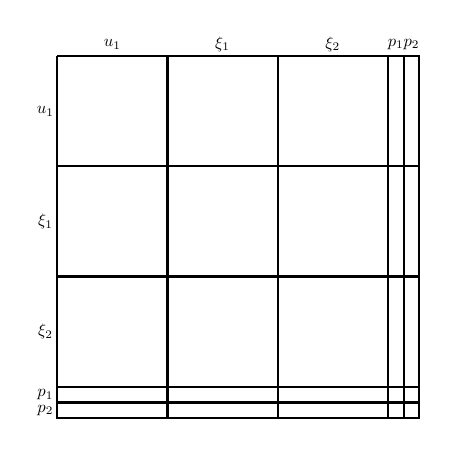
\begin{tikzpicture}[yscale=-1] 

\pgfmathsetmacro{\nt}{7};% time points
\pgfmathsetmacro{\nu}{1}; % controls
\pgfmathsetmacro{\nx}{2}; % states
\pgfmathsetmacro{\np}{2}; % parameters
\pgfmathsetmacro{\nc}{\nu + \nx}; % total continuous

%% control labels
\foreach \k in {1,...,\nu}{
	\pgfmathsetmacro{\x}{0.2*\nt*\k - 0.2/2*(\nt-1)};
	\node () at (\x,-0.05) {\scalebox{0.6}{$u_{\k}$}};
    \node () at (-0.05,\x) {\scalebox{0.6}{$u_{\k}$}};
}

%% state labels
\foreach \k in {1,...,\nx}{
	\pgfmathsetmacro{\x}{0.2*\nt*\k + 0.2*\nu*\nt - 0.2/2*(\nt-1)};
	\node () at (\x,-0.05) {\scalebox{0.6}{$\xi_{\k}$}};
    \node () at (-0.05,\x) {\scalebox{0.6}{$\xi_{\k}$}};
}

%% parameter labels
\foreach \k in {1,...,\np}{
	\pgfmathsetmacro{\x}{0.2*\k + 0.2*\nu*\nt + 0.2*\nx*\nt};
	\node () at (\x,-0.05) {\scalebox{0.6}{$p_{\k}$}};
    \node () at (-0.05,\x) {\scalebox{0.6}{$p_{\k}$}};
}


%% controls
\foreach \k in {1,...,\nu}{
	\foreach \j in {1,...,\nu}{
    \pgfmathsetmacro{\kk}{\k-1};
    \pgfmathsetmacro{\jj}{\j-1};
    \pgfmathsetmacro{\x}{0.2*\kk*\nt + 0.1};
    \pgfmathsetmacro{\y}{0.2*\jj*\nt + 0.1};
	\draw[\mysparseboxcolor,thick](\x,\y) -- (\x+0.2*\nt,\y) -- (\x+0.2*\nt,\y+0.2*\nt) -- (\x,\y+0.2*\nt) -- (\x,\y);
} }

%% states
\foreach \k in {1,...,\nx}{
	\foreach \j in {1,...,\nx}{
    \pgfmathsetmacro{\kk}{\k-1};
    \pgfmathsetmacro{\jj}{\j-1};
    \pgfmathsetmacro{\x}{0.2*\kk*\nt + 0.2*(\nu)*\nt + 0.1};
    \pgfmathsetmacro{\y}{0.2*\jj*\nt + 0.2*(\nu)*\nt + 0.1};
	\draw[\mysparseboxcolor,thick](\x,\y) -- (\x+0.2*\nt,\y) -- (\x+0.2*\nt,\y+0.2*\nt) -- (\x,\y+0.2*\nt) -- (\x,\y);
} }

%% parameters
\foreach \k in {1,...,\np}{
	\foreach \j in {1,...,\np}{
      \pgfmathsetmacro{\kk}{\k-1};
      \pgfmathsetmacro{\jj}{\j-1};
      \pgfmathsetmacro{\x}{0.2*\kk + 0.2*(\nu)*\nt + 0.2*\nx*\nt + 0.1};
      \pgfmathsetmacro{\y}{0.2*\jj + 0.2*(\nu)*\nt + 0.2*\nx*\nt + 0.1};
      \draw[\mysparseboxcolor,thick](\x,\y) -- (\x+0.2,\y) -- (\x+0.2,\y+0.2) -- (\x,\y+0.2) -- (\x,\y);
} }

%% states and controls
\foreach \k in {1,...,\nu}{
	\foreach \j in {1,...,\nx}{ 
    \pgfmathsetmacro{\kk}{\k-1};
    \pgfmathsetmacro{\jj}{\j-1};
    \pgfmathsetmacro{\x}{0.2*\kk*\nt + 0.1};
    \pgfmathsetmacro{\y}{0.2*\jj*\nt + 0.2*(\nu)*\nt + 0.1};
	\draw[\mysparseboxcolor,thick](\x,\y) -- (\x+0.2*\nt,\y) -- (\x+0.2*\nt,\y+0.2*\nt) -- (\x,\y+0.2*\nt) -- (\x,\y);
    \draw[\mysparseboxcolor,thick](\y,\x) -- (\y+0.2*\nt,\x) -- (\y+0.2*\nt,\x+0.2*\nt) -- (\y,\x+0.2*\nt) -- (\y,\x);
} }

%% states and parameters
\foreach \k in {1,...,\np}{
	\foreach \j in {1,...,\nx}{ 
    \pgfmathsetmacro{\kk}{\k-1};
    \pgfmathsetmacro{\jj}{\j-1};
    \pgfmathsetmacro{\x}{0.2*\kk + 0.2*\nx*\nt + 0.2*\nu*\nt + 0.1};
    \pgfmathsetmacro{\y}{0.2*\jj*\nt + 0.2*\nu*\nt + 0.1};
	\draw[\mysparseboxcolor,thick](\x,\y) -- (\x+0.2,\y) -- (\x+0.2,\y+0.2*\nt) -- (\x,\y+0.2*\nt) -- (\x,\y);
    \draw[\mysparseboxcolor,thick](\y,\x) -- (\y+0.2*\nt,\x) -- (\y+0.2*\nt,\x+0.2) -- (\y,\x+0.2) -- (\y,\x);

} }

%% controls and parameters
\foreach \k in {1,...,\np}{
	\foreach \j in {1,...,\nu}{
    \pgfmathsetmacro{\kk}{\k-1};
    \pgfmathsetmacro{\jj}{\j-1};
    \pgfmathsetmacro{\x}{0.2*\kk + 0.2*\nx*\nt + 0.2*\nu*\nt + 0.1};
    \pgfmathsetmacro{\y}{0.2*\jj*\nt + 0.1};
	\draw[\mysparseboxcolor,thick](\x,\y) -- (\x+0.2,\y) -- (\x+0.2,\y+0.2*\nt) -- (\x,\y+0.2*\nt) -- (\x,\y);
    \draw[\mysparseboxcolor,thick](\y,\x) -- (\y+0.2*\nt,\x) -- (\y+0.2*\nt,\x+0.2) -- (\y,\x+0.2) -- (\y,\x);
} }

%% states off 
\foreach \k in {1,...,\nx}{
	\foreach \j in {1,...,\nx}{
      \pgfmathsetmacro{\kk}{\k-1};
      \pgfmathsetmacro{\jj}{\j-1};
      \node () at ( 0.2 + 0.2*\kk*\nt + 0.2*\nu*\nt, 0.2*\nt + 0.2*\jj*\nt + 0.2*\nu*\nt ) {\mysparsesymbol};
      \node () at ( 0.2*\nt + 0.2*\jj*\nt + 0.2*\nu*\nt , 0.2 + 0.2*\kk*\nt + 0.2*\nu*\nt ) {\mysparsesymbol};
} }

%% parameters off
\foreach \k in {1,...,\np}{
	\foreach \j in {1,...,\nx}{
      \pgfmathsetmacro{\kk}{\k-1};
      \pgfmathsetmacro{\jj}{\j-1};
      \node ( ) at (0.2*\nt*\j + 0.2*\nu*\nt, 0.2*\k + 0.2*\nx*\nt + 0.2*\nu*\nt) {\mysparsesymbol};
	  \node ( ) at ( 0.2*\k + 0.2*\nx*\nt + 0.2*\nu*\nt, 0.2*\nt*\j + 0.2*\nu*\nt ) {\mysparsesymbol};
      
      \node ( ) at ( 0.2*\k + 0.2*\nx*\nt + 0.2*\nu*\nt, 0.2*\nt*\j - 0.2*\nt + 0.2 + 0.2*\nu*\nt ) {\mysparsesymbol};
      
      \node ( ) at ( 0.2*\nt*\j - 0.2*\nt + 0.2 + 0.2*\nu*\nt , 0.2*\k + 0.2*\nx*\nt + 0.2*\nu*\nt ) {\mysparsesymbol};
	  
} }

%% parameters
\foreach \k in {1,...,\np}{
      \foreach \j in {1,...,\np}{
      \pgfmathsetmacro{\kk}{\k-1};
      \pgfmathsetmacro{\jj}{\j-1};
      \node ( ) at (0.2*\j + 0.2*\nx*\nt + 0.2*\nu*\nt, 0.2*\k + 0.2*\nx*\nt + 0.2*\nu*\nt) {\mysparsesymbol};
} }

%% initial states
\foreach \k in {1,...,\nx}{
      \foreach \j in {1,...,\nx}{
      \pgfmathsetmacro{\kk}{\k-1};
      \pgfmathsetmacro{\jj}{\j-1};
      \node () at (0.2 + 0.2*\kk*\nt + 0.2*\nu*\nt, 0.2*1 + 0.2*\jj*\nt + 0.2*\nu*\nt ) {\mysparsesymbol};
} }

%% initial states
\foreach \k in {1,...,\nx}{
      \foreach \j in {1,...,\nx}{
      \pgfmathsetmacro{\kk}{\k-1};
      \pgfmathsetmacro{\jj}{\j-1};
      \node () at ( 0.2*\nt + 0.2*\kk*\nt + 0.2*\nu*\nt, 0.2*\nt + 0.2*\jj*\nt + 0.2*\nu*\nt ) {\mysparsesymbol};
} }



%% initial states
\foreach \k in {1,...,\nx}{
	\foreach \j in {1,...,\nx}{
      \pgfmathsetmacro{\kk}{\k-1};
      \pgfmathsetmacro{\jj}{\j-1};
      \node () at (0.2 + 0.2*\kk*\nt + 0.2*\nu*\nt, 0.2*1 + 0.2*\jj*\nt + 0.2*\nu*\nt ) {\mytemp};
} }
   
   
   
  
  
  
  
  
  
\end{tikzpicture}
}
% 	\end{minipage}
% }%
% \subfloat[(c) $\bm{M}_{55}$ terms.]{
% 	\begin{minipage}{0.33\textwidth}
% 	\input{../ch5/sparsity/Mxfxf}
% 	\end{minipage}
% }%

% \subfloat[(d) Remaining terms.]{
% 	\begin{minipage}{0.33\textwidth}
% 	\tikzsetnextfilename{Moff}

\centering
\resizebox{1\textwidth}{!}{
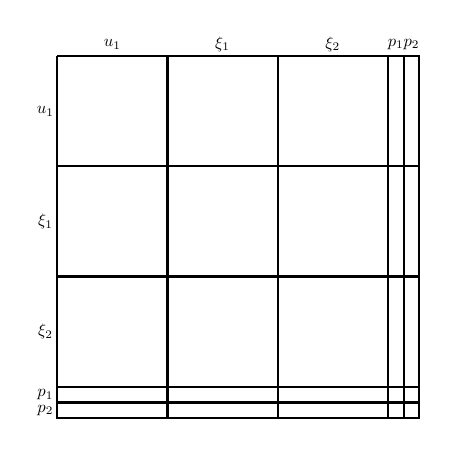
\begin{tikzpicture}[yscale=-1] 

\pgfmathsetmacro{\nt}{7};% time points
\pgfmathsetmacro{\nu}{1}; % controls
\pgfmathsetmacro{\nx}{2}; % states
\pgfmathsetmacro{\np}{2}; % parameters
\pgfmathsetmacro{\nc}{\nu + \nx}; % total continuous

%% control labels
\foreach \k in {1,...,\nu}{
	\pgfmathsetmacro{\x}{0.2*\nt*\k - 0.2/2*(\nt-1)};
	\node () at (\x,-0.05) {\scalebox{0.6}{$u_{\k}$}};
    \node () at (-0.05,\x) {\scalebox{0.6}{$u_{\k}$}};
}

%% state labels
\foreach \k in {1,...,\nx}{
	\pgfmathsetmacro{\x}{0.2*\nt*\k + 0.2*\nu*\nt - 0.2/2*(\nt-1)};
	\node () at (\x,-0.05) {\scalebox{0.6}{$\xi_{\k}$}};
    \node () at (-0.05,\x) {\scalebox{0.6}{$\xi_{\k}$}};
}

%% parameter labels
\foreach \k in {1,...,\np}{
	\pgfmathsetmacro{\x}{0.2*\k + 0.2*\nu*\nt + 0.2*\nx*\nt};
	\node () at (\x,-0.05) {\scalebox{0.6}{$p_{\k}$}};
    \node () at (-0.05,\x) {\scalebox{0.6}{$p_{\k}$}};
}


%% controls
\foreach \k in {1,...,\nu}{
	\foreach \j in {1,...,\nu}{
    \pgfmathsetmacro{\kk}{\k-1};
    \pgfmathsetmacro{\jj}{\j-1};
    \pgfmathsetmacro{\x}{0.2*\kk*\nt + 0.1};
    \pgfmathsetmacro{\y}{0.2*\jj*\nt + 0.1};
	\draw[\mysparseboxcolor,thick](\x,\y) -- (\x+0.2*\nt,\y) -- (\x+0.2*\nt,\y+0.2*\nt) -- (\x,\y+0.2*\nt) -- (\x,\y);
} }

%% states
\foreach \k in {1,...,\nx}{
	\foreach \j in {1,...,\nx}{
    \pgfmathsetmacro{\kk}{\k-1};
    \pgfmathsetmacro{\jj}{\j-1};
    \pgfmathsetmacro{\x}{0.2*\kk*\nt + 0.2*(\nu)*\nt + 0.1};
    \pgfmathsetmacro{\y}{0.2*\jj*\nt + 0.2*(\nu)*\nt + 0.1};
	\draw[\mysparseboxcolor,thick](\x,\y) -- (\x+0.2*\nt,\y) -- (\x+0.2*\nt,\y+0.2*\nt) -- (\x,\y+0.2*\nt) -- (\x,\y);
} }

%% parameters
\foreach \k in {1,...,\np}{
	\foreach \j in {1,...,\np}{
      \pgfmathsetmacro{\kk}{\k-1};
      \pgfmathsetmacro{\jj}{\j-1};
      \pgfmathsetmacro{\x}{0.2*\kk + 0.2*(\nu)*\nt + 0.2*\nx*\nt + 0.1};
      \pgfmathsetmacro{\y}{0.2*\jj + 0.2*(\nu)*\nt + 0.2*\nx*\nt + 0.1};
      \draw[\mysparseboxcolor,thick](\x,\y) -- (\x+0.2,\y) -- (\x+0.2,\y+0.2) -- (\x,\y+0.2) -- (\x,\y);
} }

%% states and controls
\foreach \k in {1,...,\nu}{
	\foreach \j in {1,...,\nx}{ 
    \pgfmathsetmacro{\kk}{\k-1};
    \pgfmathsetmacro{\jj}{\j-1};
    \pgfmathsetmacro{\x}{0.2*\kk*\nt + 0.1};
    \pgfmathsetmacro{\y}{0.2*\jj*\nt + 0.2*(\nu)*\nt + 0.1};
	\draw[\mysparseboxcolor,thick](\x,\y) -- (\x+0.2*\nt,\y) -- (\x+0.2*\nt,\y+0.2*\nt) -- (\x,\y+0.2*\nt) -- (\x,\y);
    \draw[\mysparseboxcolor,thick](\y,\x) -- (\y+0.2*\nt,\x) -- (\y+0.2*\nt,\x+0.2*\nt) -- (\y,\x+0.2*\nt) -- (\y,\x);
} }

%% states and parameters
\foreach \k in {1,...,\np}{
	\foreach \j in {1,...,\nx}{ 
    \pgfmathsetmacro{\kk}{\k-1};
    \pgfmathsetmacro{\jj}{\j-1};
    \pgfmathsetmacro{\x}{0.2*\kk + 0.2*\nx*\nt + 0.2*\nu*\nt + 0.1};
    \pgfmathsetmacro{\y}{0.2*\jj*\nt + 0.2*\nu*\nt + 0.1};
	\draw[\mysparseboxcolor,thick](\x,\y) -- (\x+0.2,\y) -- (\x+0.2,\y+0.2*\nt) -- (\x,\y+0.2*\nt) -- (\x,\y);
    \draw[\mysparseboxcolor,thick](\y,\x) -- (\y+0.2*\nt,\x) -- (\y+0.2*\nt,\x+0.2) -- (\y,\x+0.2) -- (\y,\x);

} }

%% controls and parameters
\foreach \k in {1,...,\np}{
	\foreach \j in {1,...,\nu}{
    \pgfmathsetmacro{\kk}{\k-1};
    \pgfmathsetmacro{\jj}{\j-1};
    \pgfmathsetmacro{\x}{0.2*\kk + 0.2*\nx*\nt + 0.2*\nu*\nt + 0.1};
    \pgfmathsetmacro{\y}{0.2*\jj*\nt + 0.1};
	\draw[\mysparseboxcolor,thick](\x,\y) -- (\x+0.2,\y) -- (\x+0.2,\y+0.2*\nt) -- (\x,\y+0.2*\nt) -- (\x,\y);
    \draw[\mysparseboxcolor,thick](\y,\x) -- (\y+0.2*\nt,\x) -- (\y+0.2*\nt,\x+0.2) -- (\y,\x+0.2) -- (\y,\x);
} }

%% states off 
\foreach \k in {1,...,\nx}{
	\foreach \j in {1,...,\nx}{
      \pgfmathsetmacro{\kk}{\k-1};
      \pgfmathsetmacro{\jj}{\j-1};
      \node () at ( 0.2 + 0.2*\kk*\nt + 0.2*\nu*\nt, 0.2*\nt + 0.2*\jj*\nt + 0.2*\nu*\nt ) {\mysparsesymbol};
      \node () at ( 0.2*\nt + 0.2*\jj*\nt + 0.2*\nu*\nt , 0.2 + 0.2*\kk*\nt + 0.2*\nu*\nt ) {\mysparsesymbol};
} }

%% parameters off
\foreach \k in {1,...,\np}{
	\foreach \j in {1,...,\nx}{
      \pgfmathsetmacro{\kk}{\k-1};
      \pgfmathsetmacro{\jj}{\j-1};
      \node ( ) at (0.2*\nt*\j + 0.2*\nu*\nt, 0.2*\k + 0.2*\nx*\nt + 0.2*\nu*\nt) {\mysparsesymbol};
	  \node ( ) at ( 0.2*\k + 0.2*\nx*\nt + 0.2*\nu*\nt, 0.2*\nt*\j + 0.2*\nu*\nt ) {\mysparsesymbol};
      
      \node ( ) at ( 0.2*\k + 0.2*\nx*\nt + 0.2*\nu*\nt, 0.2*\nt*\j - 0.2*\nt + 0.2 + 0.2*\nu*\nt ) {\mysparsesymbol};
      
      \node ( ) at ( 0.2*\nt*\j - 0.2*\nt + 0.2 + 0.2*\nu*\nt , 0.2*\k + 0.2*\nx*\nt + 0.2*\nu*\nt ) {\mysparsesymbol};
	  
} }

%% parameters
\foreach \k in {1,...,\np}{
      \foreach \j in {1,...,\np}{
      \pgfmathsetmacro{\kk}{\k-1};
      \pgfmathsetmacro{\jj}{\j-1};
      \node ( ) at (0.2*\j + 0.2*\nx*\nt + 0.2*\nu*\nt, 0.2*\k + 0.2*\nx*\nt + 0.2*\nu*\nt) {\mysparsesymbol};
} }

%% initial states
\foreach \k in {1,...,\nx}{
      \foreach \j in {1,...,\nx}{
      \pgfmathsetmacro{\kk}{\k-1};
      \pgfmathsetmacro{\jj}{\j-1};
      \node () at (0.2 + 0.2*\kk*\nt + 0.2*\nu*\nt, 0.2*1 + 0.2*\jj*\nt + 0.2*\nu*\nt ) {\mysparsesymbol};
} }

%% initial states
\foreach \k in {1,...,\nx}{
      \foreach \j in {1,...,\nx}{
      \pgfmathsetmacro{\kk}{\k-1};
      \pgfmathsetmacro{\jj}{\j-1};
      \node () at ( 0.2*\nt + 0.2*\kk*\nt + 0.2*\nu*\nt, 0.2*\nt + 0.2*\jj*\nt + 0.2*\nu*\nt ) {\mysparsesymbol};
} }



%% states off 
\foreach \k in {1,...,\nx}{
	\foreach \j in {1,...,\nx}{
      \pgfmathsetmacro{\kk}{\k-1};
      \pgfmathsetmacro{\jj}{\j-1};
      \node () at ( 0.2 + 0.2*\kk*\nt + 0.2*\nu*\nt, 0.2*\nt + 0.2*\jj*\nt + 0.2*\nu*\nt ) {\mytemp};
      \node () at ( 0.2*\nt + 0.2*\jj*\nt + 0.2*\nu*\nt , 0.2 + 0.2*\kk*\nt + 0.2*\nu*\nt ) {\mytemp};
} }    

%% parameters off
\foreach \k in {1,...,\np}{
	\foreach \j in {1,...,\nx}{
      \pgfmathsetmacro{\kk}{\k-1};
      \pgfmathsetmacro{\jj}{\j-1};
      \node ( ) at (0.2*\nt*\j + 0.2*\nu*\nt, 0.2*\k + 0.2*\nx*\nt + 0.2*\nu*\nt) {\mytemp};
	  \node ( ) at ( 0.2*\k + 0.2*\nx*\nt + 0.2*\nu*\nt, 0.2*\nt*\j + 0.2*\nu*\nt ) {\mytemp};
      
      \node ( ) at ( 0.2*\k + 0.2*\nx*\nt + 0.2*\nu*\nt, 0.2*\nt*\j - 0.2*\nt + 0.2 + 0.2*\nu*\nt ) {\mytemp};
      
      \node ( ) at ( 0.2*\nt*\j - 0.2*\nt + 0.2 + 0.2*\nu*\nt , 0.2*\k + 0.2*\nx*\nt + 0.2*\nu*\nt ) {\mytemp};
	  
} }





\end{tikzpicture}
}
% 	\end{minipage}
% }%

% \caption{Sparsity pattern of Mayer terms in $\mathbf{H}$ matrix.}\label{fig:figsparsityHmayer}
% \end{figure}

\begin{figure}[ht]

\centering

\begin{subfigure}{0.33\textwidth}
\centering
\begin{minipage}{\textwidth}
\tikzsetnextfilename{ASSTheta1}

\centering
\resizebox{1\textwidth}{!}{
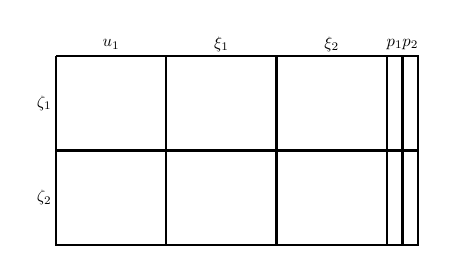
\begin{tikzpicture}[yscale=-1] 

\pgfmathsetmacro{\nt}{7};% time points
\pgfmathsetmacro{\ntm}{\nt-1};
\pgfmathsetmacro{\nu}{1}; % controls
\pgfmathsetmacro{\nx}{2}; % states
\pgfmathsetmacro{\np}{2}; % parameters
\pgfmathsetmacro{\nc}{\nu + \nx}; % total continuous

%% control labels
\foreach \k in {1,...,\nu}{
	\pgfmathsetmacro{\x}{0.2*\nt*\k - 0.2/2*(\nt-1)};
	\node () at (\x,-0.05) {\scalebox{0.6}{$u_{\k}$}};
}

%% state labels
\foreach \k in {1,...,\nx}{
	\pgfmathsetmacro{\x}{0.2*\nt*\k + 0.2*\nu*\nt - 0.2/2*(\nt-1)};
	\node () at (\x,-0.05) {\scalebox{0.6}{$\xi_{\k}$}};
}

%% parameter labels
\foreach \k in {1,...,\np}{
	\pgfmathsetmacro{\x}{0.2*\k + 0.2*\nu*\nt + 0.2*\nx*\nt};
	\node () at (\x,-0.05) {\scalebox{0.6}{$p_{\k}$}};
}

%% defects
\foreach \k in {1,...,\nx}{
	\pgfmathsetmacro{\x}{0.2*\ntm*\k - 0.2/2*(\ntm-1)};
	\node () at (-0.05,\x) {\scalebox{0.6}{$\zeta_{\k}$}};
}


%% controls
\foreach \k in {1,...,\nu}{
	\foreach \j in {1,...,\nx}{
		\foreach \i in {1,...,\ntm}{ 
        	\pgfmathsetmacro{\kk}{\k-1};
            \pgfmathsetmacro{\jj}{\j-1};
        	\pgfmathsetmacro{\x}{0.2*\i + 0.2*\kk*\nt};
            \pgfmathsetmacro{\y}{0.2*\i + 0.2*\jj*\ntm};
        	\node () at (\x,\y) {\mysparsesymbol};
            \node () at (\x+0.2,\y) {\mysparsesymbol};
} 
    \pgfmathsetmacro{\kk}{\k-1};
    \pgfmathsetmacro{\jj}{\j-1};
    \pgfmathsetmacro{\x}{0.2*\kk*\nt + 0.1};
    \pgfmathsetmacro{\y}{0.2*\jj*\ntm + 0.1};
	\draw[\mysparseboxcolor,thick](\x,\y) -- (\x+0.2*\nt,\y) -- (\x+0.2*\nt,\y+0.2*\ntm) -- (\x,\y+0.2*\ntm) -- (\x,\y);
} }

%% states
\foreach \k in {1,...,\nx}{
	\foreach \j in {1,...,\nx}{
		\foreach \i in {1,...,\ntm}{ 
        	\pgfmathsetmacro{\kk}{\k-1};
            \pgfmathsetmacro{\jj}{\j-1};
        	\pgfmathsetmacro{\x}{0.2*\i + 0.2*\nu*\nt + 0.2*\kk*\nt};
            \pgfmathsetmacro{\y}{0.2*\i + 0.2*\jj*\ntm};
        	\node () at (\x,\y) {\mysparsesymbol};
            \node () at (\x+0.2,\y) {\mysparsesymbol};
} 
    \pgfmathsetmacro{\kk}{\k-1};
    \pgfmathsetmacro{\jj}{\j-1};
    \pgfmathsetmacro{\x}{0.2*\kk*\nt + 0.2*\nu*\nt + 0.1};
    \pgfmathsetmacro{\y}{0.2*\jj*\ntm + 0.1};
	\draw[\mysparseboxcolor,thick](\x,\y) -- (\x+0.2*\nt,\y) -- (\x+0.2*\nt,\y+0.2*\ntm) -- (\x,\y+0.2*\ntm) -- (\x,\y);
} }

%% states and parameters
\foreach \k in {1,...,\np}{
	\foreach \j in {1,...,\nx}{
		\foreach \i in {1,...,\ntm}{ 
        	\pgfmathsetmacro{\kk}{\k-1};
            \pgfmathsetmacro{\jj}{\j-1};
        	\node () at ( 0.2*\k + 0.2*\nx*\nt + 0.2*\nu*\nt, 0.2*\i + 0.2*\jj*\ntm ) {\mysparsesymbol};
} 
    \pgfmathsetmacro{\kk}{\k-1};
    \pgfmathsetmacro{\jj}{\j-1};
    \pgfmathsetmacro{\x}{0.2*\kk + 0.2*\nx*\nt + 0.2*\nu*\nt + 0.1};
    \pgfmathsetmacro{\y}{0.2*\jj*\ntm+ 0.1};
	\draw[\mysparseboxcolor,thick](\x,\y) -- (\x+0.2,\y) -- (\x+0.2,\y+0.2*\ntm) -- (\x,\y+0.2*\ntm) -- (\x,\y);
} }

%% states
\foreach \k in {1,...,\nx}{
	\foreach \j in {1,...,\nx}{
		\foreach \i in {1,...,\ntm}{ 
        	\pgfmathsetmacro{\kk}{\k-1};
            \pgfmathsetmacro{\jj}{\j-1};
        	\pgfmathsetmacro{\x}{0.2*\i + 0.2*\nu*\nt + 0.2*\kk*\nt};
            \pgfmathsetmacro{\y}{0.2*\i + 0.2*\jj*\ntm};
        	\node () at (\x,\y) {\mytemp};
} } }

\end{tikzpicture}
}
\end{minipage}
\caption{$\bm{\theta}_1$ terms.}
% \label{fig:}
\end{subfigure}%
\begin{subfigure}{0.33\textwidth}
\centering
\begin{minipage}{\textwidth}
\input{../ch5/sparsity/ASSTheta2}
\end{minipage}
\caption{$\bm{\theta}_2$ terms.}
% \label{fig:}
\end{subfigure}%
\begin{subfigure}{0.33\textwidth}
\centering
\begin{minipage}{\textwidth}
\input{../ch5/sparsity/ASSTheta3}
\end{minipage}
\caption{$\bm{\theta}_3$ terms.}
% \label{fig:}
\end{subfigure}%

\begin{subfigure}{0.33\textwidth}
\centering
\begin{minipage}{\textwidth}
\tikzsetnextfilename{ASSTheta4}

\centering
\resizebox{1\textwidth}{!}{
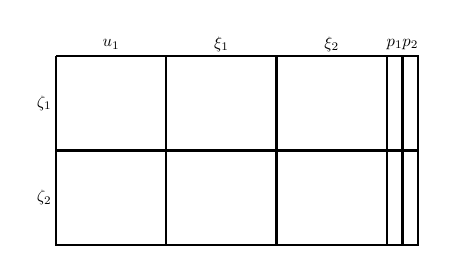
\begin{tikzpicture}[yscale=-1] 

\pgfmathsetmacro{\nt}{7};% time points
\pgfmathsetmacro{\ntm}{\nt-1};
\pgfmathsetmacro{\nu}{1}; % controls
\pgfmathsetmacro{\nx}{2}; % states
\pgfmathsetmacro{\np}{2}; % parameters
\pgfmathsetmacro{\nc}{\nu + \nx}; % total continuous

%% control labels
\foreach \k in {1,...,\nu}{
	\pgfmathsetmacro{\x}{0.2*\nt*\k - 0.2/2*(\nt-1)};
	\node () at (\x,-0.05) {\scalebox{0.6}{$u_{\k}$}};
}

%% state labels
\foreach \k in {1,...,\nx}{
	\pgfmathsetmacro{\x}{0.2*\nt*\k + 0.2*\nu*\nt - 0.2/2*(\nt-1)};
	\node () at (\x,-0.05) {\scalebox{0.6}{$\xi_{\k}$}};
}

%% parameter labels
\foreach \k in {1,...,\np}{
	\pgfmathsetmacro{\x}{0.2*\k + 0.2*\nu*\nt + 0.2*\nx*\nt};
	\node () at (\x,-0.05) {\scalebox{0.6}{$p_{\k}$}};
}

%% defects
\foreach \k in {1,...,\nx}{
	\pgfmathsetmacro{\x}{0.2*\ntm*\k - 0.2/2*(\ntm-1)};
	\node () at (-0.05,\x) {\scalebox{0.6}{$\zeta_{\k}$}};
}


%% controls
\foreach \k in {1,...,\nu}{
	\foreach \j in {1,...,\nx}{
		\foreach \i in {1,...,\ntm}{ 
        	\pgfmathsetmacro{\kk}{\k-1};
            \pgfmathsetmacro{\jj}{\j-1};
        	\pgfmathsetmacro{\x}{0.2*\i + 0.2*\kk*\nt};
            \pgfmathsetmacro{\y}{0.2*\i + 0.2*\jj*\ntm};
        	\node () at (\x,\y) {\mysparsesymbol};
            \node () at (\x+0.2,\y) {\mysparsesymbol};
} 
    \pgfmathsetmacro{\kk}{\k-1};
    \pgfmathsetmacro{\jj}{\j-1};
    \pgfmathsetmacro{\x}{0.2*\kk*\nt + 0.1};
    \pgfmathsetmacro{\y}{0.2*\jj*\ntm + 0.1};
	\draw[\mysparseboxcolor,thick](\x,\y) -- (\x+0.2*\nt,\y) -- (\x+0.2*\nt,\y+0.2*\ntm) -- (\x,\y+0.2*\ntm) -- (\x,\y);
} }

%% states
\foreach \k in {1,...,\nx}{
	\foreach \j in {1,...,\nx}{
		\foreach \i in {1,...,\ntm}{ 
        	\pgfmathsetmacro{\kk}{\k-1};
            \pgfmathsetmacro{\jj}{\j-1};
        	\pgfmathsetmacro{\x}{0.2*\i + 0.2*\nu*\nt + 0.2*\kk*\nt};
            \pgfmathsetmacro{\y}{0.2*\i + 0.2*\jj*\ntm};
        	\node () at (\x,\y) {\mysparsesymbol};
            \node () at (\x+0.2,\y) {\mysparsesymbol};
} 
    \pgfmathsetmacro{\kk}{\k-1};
    \pgfmathsetmacro{\jj}{\j-1};
    \pgfmathsetmacro{\x}{0.2*\kk*\nt + 0.2*\nu*\nt + 0.1};
    \pgfmathsetmacro{\y}{0.2*\jj*\ntm + 0.1};
	\draw[\mysparseboxcolor,thick](\x,\y) -- (\x+0.2*\nt,\y) -- (\x+0.2*\nt,\y+0.2*\ntm) -- (\x,\y+0.2*\ntm) -- (\x,\y);
} }

%% states and parameters
\foreach \k in {1,...,\np}{
	\foreach \j in {1,...,\nx}{
		\foreach \i in {1,...,\ntm}{ 
        	\pgfmathsetmacro{\kk}{\k-1};
            \pgfmathsetmacro{\jj}{\j-1};
        	\node () at ( 0.2*\k + 0.2*\nx*\nt + 0.2*\nu*\nt, 0.2*\i + 0.2*\jj*\ntm ) {\mysparsesymbol};
} 
    \pgfmathsetmacro{\kk}{\k-1};
    \pgfmathsetmacro{\jj}{\j-1};
    \pgfmathsetmacro{\x}{0.2*\kk + 0.2*\nx*\nt + 0.2*\nu*\nt + 0.1};
    \pgfmathsetmacro{\y}{0.2*\jj*\ntm+ 0.1};
	\draw[\mysparseboxcolor,thick](\x,\y) -- (\x+0.2,\y) -- (\x+0.2,\y+0.2*\ntm) -- (\x,\y+0.2*\ntm) -- (\x,\y);
} }

%% controls
\foreach \k in {1,...,\nu}{
	\foreach \j in {1,...,\nx}{
		\foreach \i in {1,...,\ntm}{ 
        	\pgfmathsetmacro{\kk}{\k-1};
            \pgfmathsetmacro{\jj}{\j-1};
        	\pgfmathsetmacro{\x}{0.2*\i + 0.2*\kk*\nt};
            \pgfmathsetmacro{\y}{0.2*\i + 0.2*\jj*\ntm};
            \node () at (\x+0.2,\y) {\mytemp};
} } }

\end{tikzpicture}
}
\end{minipage}
\caption{$\bm{\theta}_4$ terms.}
% \label{fig:}
\end{subfigure}%
\begin{subfigure}{0.33\textwidth}
\centering
\begin{minipage}{\textwidth}
\tikzsetnextfilename{ASSTheta5}

\centering
\resizebox{1\textwidth}{!}{
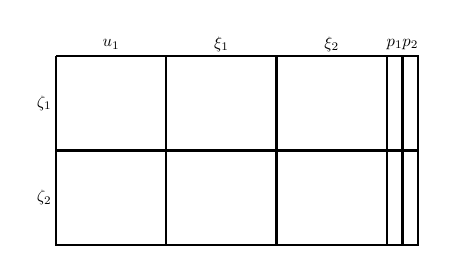
\begin{tikzpicture}[yscale=-1] 

\pgfmathsetmacro{\nt}{7};% time points
\pgfmathsetmacro{\ntm}{\nt-1};
\pgfmathsetmacro{\nu}{1}; % controls
\pgfmathsetmacro{\nx}{2}; % states
\pgfmathsetmacro{\np}{2}; % parameters
\pgfmathsetmacro{\nc}{\nu + \nx}; % total continuous

%% control labels
\foreach \k in {1,...,\nu}{
	\pgfmathsetmacro{\x}{0.2*\nt*\k - 0.2/2*(\nt-1)};
	\node () at (\x,-0.05) {\scalebox{0.6}{$u_{\k}$}};
}

%% state labels
\foreach \k in {1,...,\nx}{
	\pgfmathsetmacro{\x}{0.2*\nt*\k + 0.2*\nu*\nt - 0.2/2*(\nt-1)};
	\node () at (\x,-0.05) {\scalebox{0.6}{$\xi_{\k}$}};
}

%% parameter labels
\foreach \k in {1,...,\np}{
	\pgfmathsetmacro{\x}{0.2*\k + 0.2*\nu*\nt + 0.2*\nx*\nt};
	\node () at (\x,-0.05) {\scalebox{0.6}{$p_{\k}$}};
}

%% defects
\foreach \k in {1,...,\nx}{
	\pgfmathsetmacro{\x}{0.2*\ntm*\k - 0.2/2*(\ntm-1)};
	\node () at (-0.05,\x) {\scalebox{0.6}{$\zeta_{\k}$}};
}


%% controls
\foreach \k in {1,...,\nu}{
	\foreach \j in {1,...,\nx}{
		\foreach \i in {1,...,\ntm}{ 
        	\pgfmathsetmacro{\kk}{\k-1};
            \pgfmathsetmacro{\jj}{\j-1};
        	\pgfmathsetmacro{\x}{0.2*\i + 0.2*\kk*\nt};
            \pgfmathsetmacro{\y}{0.2*\i + 0.2*\jj*\ntm};
        	\node () at (\x,\y) {\mysparsesymbol};
            \node () at (\x+0.2,\y) {\mysparsesymbol};
} 
    \pgfmathsetmacro{\kk}{\k-1};
    \pgfmathsetmacro{\jj}{\j-1};
    \pgfmathsetmacro{\x}{0.2*\kk*\nt + 0.1};
    \pgfmathsetmacro{\y}{0.2*\jj*\ntm + 0.1};
	\draw[\mysparseboxcolor,thick](\x,\y) -- (\x+0.2*\nt,\y) -- (\x+0.2*\nt,\y+0.2*\ntm) -- (\x,\y+0.2*\ntm) -- (\x,\y);
} }

%% states
\foreach \k in {1,...,\nx}{
	\foreach \j in {1,...,\nx}{
		\foreach \i in {1,...,\ntm}{ 
        	\pgfmathsetmacro{\kk}{\k-1};
            \pgfmathsetmacro{\jj}{\j-1};
        	\pgfmathsetmacro{\x}{0.2*\i + 0.2*\nu*\nt + 0.2*\kk*\nt};
            \pgfmathsetmacro{\y}{0.2*\i + 0.2*\jj*\ntm};
        	\node () at (\x,\y) {\mysparsesymbol};
            \node () at (\x+0.2,\y) {\mysparsesymbol};
} 
    \pgfmathsetmacro{\kk}{\k-1};
    \pgfmathsetmacro{\jj}{\j-1};
    \pgfmathsetmacro{\x}{0.2*\kk*\nt + 0.2*\nu*\nt + 0.1};
    \pgfmathsetmacro{\y}{0.2*\jj*\ntm + 0.1};
	\draw[\mysparseboxcolor,thick](\x,\y) -- (\x+0.2*\nt,\y) -- (\x+0.2*\nt,\y+0.2*\ntm) -- (\x,\y+0.2*\ntm) -- (\x,\y);
} }

%% states and parameters
\foreach \k in {1,...,\np}{
	\foreach \j in {1,...,\nx}{
		\foreach \i in {1,...,\ntm}{ 
        	\pgfmathsetmacro{\kk}{\k-1};
            \pgfmathsetmacro{\jj}{\j-1};
        	\node () at ( 0.2*\k + 0.2*\nx*\nt + 0.2*\nu*\nt, 0.2*\i + 0.2*\jj*\ntm ) {\mysparsesymbol};
} 
    \pgfmathsetmacro{\kk}{\k-1};
    \pgfmathsetmacro{\jj}{\j-1};
    \pgfmathsetmacro{\x}{0.2*\kk + 0.2*\nx*\nt + 0.2*\nu*\nt + 0.1};
    \pgfmathsetmacro{\y}{0.2*\jj*\ntm+ 0.1};
	\draw[\mysparseboxcolor,thick](\x,\y) -- (\x+0.2,\y) -- (\x+0.2,\y+0.2*\ntm) -- (\x,\y+0.2*\ntm) -- (\x,\y);
} }

%% states and parameters
\foreach \k in {1,...,\np}{
	\foreach \j in {1,...,\nx}{
		\foreach \i in {1,...,\ntm}{ 
        	\pgfmathsetmacro{\kk}{\k-1};
            \pgfmathsetmacro{\jj}{\j-1};
        	\node () at ( 0.2*\k + 0.2*\nx*\nt + 0.2*\nu*\nt, 0.2*\i + 0.2*\jj*\ntm ) {\mytemp};
} } }

\end{tikzpicture}
}
\end{minipage}
\caption{$\bm{\theta}_5$ terms.}
% \label{fig:}
\end{subfigure}%

\caption{Sparsity pattern of $\mathbf{A}_{e1}$ matrix for the defect constraints using a single-step method.}\label{fig:figsparsityASS}
\end{figure}


% \begin{figure}[h]

% \centering

% \subfloat[(a) $\bm{\theta}_1$ terms.]{
% 	\begin{minipage}{0.33\textwidth}
% 	\tikzsetnextfilename{ASSTheta1}

\centering
\resizebox{1\textwidth}{!}{
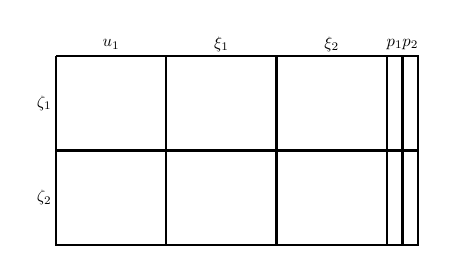
\begin{tikzpicture}[yscale=-1] 

\pgfmathsetmacro{\nt}{7};% time points
\pgfmathsetmacro{\ntm}{\nt-1};
\pgfmathsetmacro{\nu}{1}; % controls
\pgfmathsetmacro{\nx}{2}; % states
\pgfmathsetmacro{\np}{2}; % parameters
\pgfmathsetmacro{\nc}{\nu + \nx}; % total continuous

%% control labels
\foreach \k in {1,...,\nu}{
	\pgfmathsetmacro{\x}{0.2*\nt*\k - 0.2/2*(\nt-1)};
	\node () at (\x,-0.05) {\scalebox{0.6}{$u_{\k}$}};
}

%% state labels
\foreach \k in {1,...,\nx}{
	\pgfmathsetmacro{\x}{0.2*\nt*\k + 0.2*\nu*\nt - 0.2/2*(\nt-1)};
	\node () at (\x,-0.05) {\scalebox{0.6}{$\xi_{\k}$}};
}

%% parameter labels
\foreach \k in {1,...,\np}{
	\pgfmathsetmacro{\x}{0.2*\k + 0.2*\nu*\nt + 0.2*\nx*\nt};
	\node () at (\x,-0.05) {\scalebox{0.6}{$p_{\k}$}};
}

%% defects
\foreach \k in {1,...,\nx}{
	\pgfmathsetmacro{\x}{0.2*\ntm*\k - 0.2/2*(\ntm-1)};
	\node () at (-0.05,\x) {\scalebox{0.6}{$\zeta_{\k}$}};
}


%% controls
\foreach \k in {1,...,\nu}{
	\foreach \j in {1,...,\nx}{
		\foreach \i in {1,...,\ntm}{ 
        	\pgfmathsetmacro{\kk}{\k-1};
            \pgfmathsetmacro{\jj}{\j-1};
        	\pgfmathsetmacro{\x}{0.2*\i + 0.2*\kk*\nt};
            \pgfmathsetmacro{\y}{0.2*\i + 0.2*\jj*\ntm};
        	\node () at (\x,\y) {\mysparsesymbol};
            \node () at (\x+0.2,\y) {\mysparsesymbol};
} 
    \pgfmathsetmacro{\kk}{\k-1};
    \pgfmathsetmacro{\jj}{\j-1};
    \pgfmathsetmacro{\x}{0.2*\kk*\nt + 0.1};
    \pgfmathsetmacro{\y}{0.2*\jj*\ntm + 0.1};
	\draw[\mysparseboxcolor,thick](\x,\y) -- (\x+0.2*\nt,\y) -- (\x+0.2*\nt,\y+0.2*\ntm) -- (\x,\y+0.2*\ntm) -- (\x,\y);
} }

%% states
\foreach \k in {1,...,\nx}{
	\foreach \j in {1,...,\nx}{
		\foreach \i in {1,...,\ntm}{ 
        	\pgfmathsetmacro{\kk}{\k-1};
            \pgfmathsetmacro{\jj}{\j-1};
        	\pgfmathsetmacro{\x}{0.2*\i + 0.2*\nu*\nt + 0.2*\kk*\nt};
            \pgfmathsetmacro{\y}{0.2*\i + 0.2*\jj*\ntm};
        	\node () at (\x,\y) {\mysparsesymbol};
            \node () at (\x+0.2,\y) {\mysparsesymbol};
} 
    \pgfmathsetmacro{\kk}{\k-1};
    \pgfmathsetmacro{\jj}{\j-1};
    \pgfmathsetmacro{\x}{0.2*\kk*\nt + 0.2*\nu*\nt + 0.1};
    \pgfmathsetmacro{\y}{0.2*\jj*\ntm + 0.1};
	\draw[\mysparseboxcolor,thick](\x,\y) -- (\x+0.2*\nt,\y) -- (\x+0.2*\nt,\y+0.2*\ntm) -- (\x,\y+0.2*\ntm) -- (\x,\y);
} }

%% states and parameters
\foreach \k in {1,...,\np}{
	\foreach \j in {1,...,\nx}{
		\foreach \i in {1,...,\ntm}{ 
        	\pgfmathsetmacro{\kk}{\k-1};
            \pgfmathsetmacro{\jj}{\j-1};
        	\node () at ( 0.2*\k + 0.2*\nx*\nt + 0.2*\nu*\nt, 0.2*\i + 0.2*\jj*\ntm ) {\mysparsesymbol};
} 
    \pgfmathsetmacro{\kk}{\k-1};
    \pgfmathsetmacro{\jj}{\j-1};
    \pgfmathsetmacro{\x}{0.2*\kk + 0.2*\nx*\nt + 0.2*\nu*\nt + 0.1};
    \pgfmathsetmacro{\y}{0.2*\jj*\ntm+ 0.1};
	\draw[\mysparseboxcolor,thick](\x,\y) -- (\x+0.2,\y) -- (\x+0.2,\y+0.2*\ntm) -- (\x,\y+0.2*\ntm) -- (\x,\y);
} }

%% states
\foreach \k in {1,...,\nx}{
	\foreach \j in {1,...,\nx}{
		\foreach \i in {1,...,\ntm}{ 
        	\pgfmathsetmacro{\kk}{\k-1};
            \pgfmathsetmacro{\jj}{\j-1};
        	\pgfmathsetmacro{\x}{0.2*\i + 0.2*\nu*\nt + 0.2*\kk*\nt};
            \pgfmathsetmacro{\y}{0.2*\i + 0.2*\jj*\ntm};
        	\node () at (\x,\y) {\mytemp};
} } }

\end{tikzpicture}
}
% 	\end{minipage}
% }%
% \subfloat[(b) $\bm{\theta}_2$ terms.]{
% 	\begin{minipage}{0.33\textwidth}
% 	\input{../ch5/sparsity/ASSTheta2}
% 	\end{minipage}
% }%
% \subfloat[(c) $\bm{\theta}_3$ terms.]{
% 	\begin{minipage}{0.33\textwidth}
% 	\input{../ch5/sparsity/ASSTheta3}
% 	\end{minipage}
% }%

% \subfloat[(d) $\bm{\theta}_4$ terms.]{
% 	\begin{minipage}{0.33\textwidth}
% 	\tikzsetnextfilename{ASSTheta4}

\centering
\resizebox{1\textwidth}{!}{
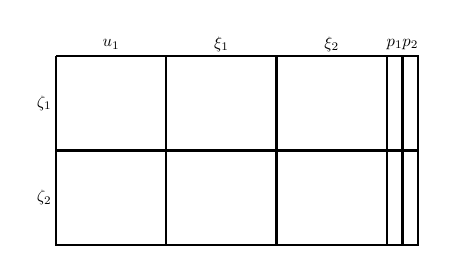
\begin{tikzpicture}[yscale=-1] 

\pgfmathsetmacro{\nt}{7};% time points
\pgfmathsetmacro{\ntm}{\nt-1};
\pgfmathsetmacro{\nu}{1}; % controls
\pgfmathsetmacro{\nx}{2}; % states
\pgfmathsetmacro{\np}{2}; % parameters
\pgfmathsetmacro{\nc}{\nu + \nx}; % total continuous

%% control labels
\foreach \k in {1,...,\nu}{
	\pgfmathsetmacro{\x}{0.2*\nt*\k - 0.2/2*(\nt-1)};
	\node () at (\x,-0.05) {\scalebox{0.6}{$u_{\k}$}};
}

%% state labels
\foreach \k in {1,...,\nx}{
	\pgfmathsetmacro{\x}{0.2*\nt*\k + 0.2*\nu*\nt - 0.2/2*(\nt-1)};
	\node () at (\x,-0.05) {\scalebox{0.6}{$\xi_{\k}$}};
}

%% parameter labels
\foreach \k in {1,...,\np}{
	\pgfmathsetmacro{\x}{0.2*\k + 0.2*\nu*\nt + 0.2*\nx*\nt};
	\node () at (\x,-0.05) {\scalebox{0.6}{$p_{\k}$}};
}

%% defects
\foreach \k in {1,...,\nx}{
	\pgfmathsetmacro{\x}{0.2*\ntm*\k - 0.2/2*(\ntm-1)};
	\node () at (-0.05,\x) {\scalebox{0.6}{$\zeta_{\k}$}};
}


%% controls
\foreach \k in {1,...,\nu}{
	\foreach \j in {1,...,\nx}{
		\foreach \i in {1,...,\ntm}{ 
        	\pgfmathsetmacro{\kk}{\k-1};
            \pgfmathsetmacro{\jj}{\j-1};
        	\pgfmathsetmacro{\x}{0.2*\i + 0.2*\kk*\nt};
            \pgfmathsetmacro{\y}{0.2*\i + 0.2*\jj*\ntm};
        	\node () at (\x,\y) {\mysparsesymbol};
            \node () at (\x+0.2,\y) {\mysparsesymbol};
} 
    \pgfmathsetmacro{\kk}{\k-1};
    \pgfmathsetmacro{\jj}{\j-1};
    \pgfmathsetmacro{\x}{0.2*\kk*\nt + 0.1};
    \pgfmathsetmacro{\y}{0.2*\jj*\ntm + 0.1};
	\draw[\mysparseboxcolor,thick](\x,\y) -- (\x+0.2*\nt,\y) -- (\x+0.2*\nt,\y+0.2*\ntm) -- (\x,\y+0.2*\ntm) -- (\x,\y);
} }

%% states
\foreach \k in {1,...,\nx}{
	\foreach \j in {1,...,\nx}{
		\foreach \i in {1,...,\ntm}{ 
        	\pgfmathsetmacro{\kk}{\k-1};
            \pgfmathsetmacro{\jj}{\j-1};
        	\pgfmathsetmacro{\x}{0.2*\i + 0.2*\nu*\nt + 0.2*\kk*\nt};
            \pgfmathsetmacro{\y}{0.2*\i + 0.2*\jj*\ntm};
        	\node () at (\x,\y) {\mysparsesymbol};
            \node () at (\x+0.2,\y) {\mysparsesymbol};
} 
    \pgfmathsetmacro{\kk}{\k-1};
    \pgfmathsetmacro{\jj}{\j-1};
    \pgfmathsetmacro{\x}{0.2*\kk*\nt + 0.2*\nu*\nt + 0.1};
    \pgfmathsetmacro{\y}{0.2*\jj*\ntm + 0.1};
	\draw[\mysparseboxcolor,thick](\x,\y) -- (\x+0.2*\nt,\y) -- (\x+0.2*\nt,\y+0.2*\ntm) -- (\x,\y+0.2*\ntm) -- (\x,\y);
} }

%% states and parameters
\foreach \k in {1,...,\np}{
	\foreach \j in {1,...,\nx}{
		\foreach \i in {1,...,\ntm}{ 
        	\pgfmathsetmacro{\kk}{\k-1};
            \pgfmathsetmacro{\jj}{\j-1};
        	\node () at ( 0.2*\k + 0.2*\nx*\nt + 0.2*\nu*\nt, 0.2*\i + 0.2*\jj*\ntm ) {\mysparsesymbol};
} 
    \pgfmathsetmacro{\kk}{\k-1};
    \pgfmathsetmacro{\jj}{\j-1};
    \pgfmathsetmacro{\x}{0.2*\kk + 0.2*\nx*\nt + 0.2*\nu*\nt + 0.1};
    \pgfmathsetmacro{\y}{0.2*\jj*\ntm+ 0.1};
	\draw[\mysparseboxcolor,thick](\x,\y) -- (\x+0.2,\y) -- (\x+0.2,\y+0.2*\ntm) -- (\x,\y+0.2*\ntm) -- (\x,\y);
} }

%% controls
\foreach \k in {1,...,\nu}{
	\foreach \j in {1,...,\nx}{
		\foreach \i in {1,...,\ntm}{ 
        	\pgfmathsetmacro{\kk}{\k-1};
            \pgfmathsetmacro{\jj}{\j-1};
        	\pgfmathsetmacro{\x}{0.2*\i + 0.2*\kk*\nt};
            \pgfmathsetmacro{\y}{0.2*\i + 0.2*\jj*\ntm};
            \node () at (\x+0.2,\y) {\mytemp};
} } }

\end{tikzpicture}
}
% 	\end{minipage}
% }%
% \subfloat[(e) $\bm{\theta}_5$ terms.]{
% 	\begin{minipage}{0.33\textwidth}
% 	\tikzsetnextfilename{ASSTheta5}

\centering
\resizebox{1\textwidth}{!}{
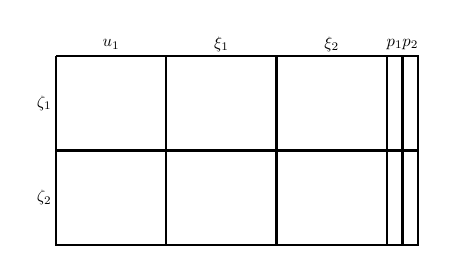
\begin{tikzpicture}[yscale=-1] 

\pgfmathsetmacro{\nt}{7};% time points
\pgfmathsetmacro{\ntm}{\nt-1};
\pgfmathsetmacro{\nu}{1}; % controls
\pgfmathsetmacro{\nx}{2}; % states
\pgfmathsetmacro{\np}{2}; % parameters
\pgfmathsetmacro{\nc}{\nu + \nx}; % total continuous

%% control labels
\foreach \k in {1,...,\nu}{
	\pgfmathsetmacro{\x}{0.2*\nt*\k - 0.2/2*(\nt-1)};
	\node () at (\x,-0.05) {\scalebox{0.6}{$u_{\k}$}};
}

%% state labels
\foreach \k in {1,...,\nx}{
	\pgfmathsetmacro{\x}{0.2*\nt*\k + 0.2*\nu*\nt - 0.2/2*(\nt-1)};
	\node () at (\x,-0.05) {\scalebox{0.6}{$\xi_{\k}$}};
}

%% parameter labels
\foreach \k in {1,...,\np}{
	\pgfmathsetmacro{\x}{0.2*\k + 0.2*\nu*\nt + 0.2*\nx*\nt};
	\node () at (\x,-0.05) {\scalebox{0.6}{$p_{\k}$}};
}

%% defects
\foreach \k in {1,...,\nx}{
	\pgfmathsetmacro{\x}{0.2*\ntm*\k - 0.2/2*(\ntm-1)};
	\node () at (-0.05,\x) {\scalebox{0.6}{$\zeta_{\k}$}};
}


%% controls
\foreach \k in {1,...,\nu}{
	\foreach \j in {1,...,\nx}{
		\foreach \i in {1,...,\ntm}{ 
        	\pgfmathsetmacro{\kk}{\k-1};
            \pgfmathsetmacro{\jj}{\j-1};
        	\pgfmathsetmacro{\x}{0.2*\i + 0.2*\kk*\nt};
            \pgfmathsetmacro{\y}{0.2*\i + 0.2*\jj*\ntm};
        	\node () at (\x,\y) {\mysparsesymbol};
            \node () at (\x+0.2,\y) {\mysparsesymbol};
} 
    \pgfmathsetmacro{\kk}{\k-1};
    \pgfmathsetmacro{\jj}{\j-1};
    \pgfmathsetmacro{\x}{0.2*\kk*\nt + 0.1};
    \pgfmathsetmacro{\y}{0.2*\jj*\ntm + 0.1};
	\draw[\mysparseboxcolor,thick](\x,\y) -- (\x+0.2*\nt,\y) -- (\x+0.2*\nt,\y+0.2*\ntm) -- (\x,\y+0.2*\ntm) -- (\x,\y);
} }

%% states
\foreach \k in {1,...,\nx}{
	\foreach \j in {1,...,\nx}{
		\foreach \i in {1,...,\ntm}{ 
        	\pgfmathsetmacro{\kk}{\k-1};
            \pgfmathsetmacro{\jj}{\j-1};
        	\pgfmathsetmacro{\x}{0.2*\i + 0.2*\nu*\nt + 0.2*\kk*\nt};
            \pgfmathsetmacro{\y}{0.2*\i + 0.2*\jj*\ntm};
        	\node () at (\x,\y) {\mysparsesymbol};
            \node () at (\x+0.2,\y) {\mysparsesymbol};
} 
    \pgfmathsetmacro{\kk}{\k-1};
    \pgfmathsetmacro{\jj}{\j-1};
    \pgfmathsetmacro{\x}{0.2*\kk*\nt + 0.2*\nu*\nt + 0.1};
    \pgfmathsetmacro{\y}{0.2*\jj*\ntm + 0.1};
	\draw[\mysparseboxcolor,thick](\x,\y) -- (\x+0.2*\nt,\y) -- (\x+0.2*\nt,\y+0.2*\ntm) -- (\x,\y+0.2*\ntm) -- (\x,\y);
} }

%% states and parameters
\foreach \k in {1,...,\np}{
	\foreach \j in {1,...,\nx}{
		\foreach \i in {1,...,\ntm}{ 
        	\pgfmathsetmacro{\kk}{\k-1};
            \pgfmathsetmacro{\jj}{\j-1};
        	\node () at ( 0.2*\k + 0.2*\nx*\nt + 0.2*\nu*\nt, 0.2*\i + 0.2*\jj*\ntm ) {\mysparsesymbol};
} 
    \pgfmathsetmacro{\kk}{\k-1};
    \pgfmathsetmacro{\jj}{\j-1};
    \pgfmathsetmacro{\x}{0.2*\kk + 0.2*\nx*\nt + 0.2*\nu*\nt + 0.1};
    \pgfmathsetmacro{\y}{0.2*\jj*\ntm+ 0.1};
	\draw[\mysparseboxcolor,thick](\x,\y) -- (\x+0.2,\y) -- (\x+0.2,\y+0.2*\ntm) -- (\x,\y+0.2*\ntm) -- (\x,\y);
} }

%% states and parameters
\foreach \k in {1,...,\np}{
	\foreach \j in {1,...,\nx}{
		\foreach \i in {1,...,\ntm}{ 
        	\pgfmathsetmacro{\kk}{\k-1};
            \pgfmathsetmacro{\jj}{\j-1};
        	\node () at ( 0.2*\k + 0.2*\nx*\nt + 0.2*\nu*\nt, 0.2*\i + 0.2*\jj*\ntm ) {\mytemp};
} } }

\end{tikzpicture}
}
% 	\end{minipage}
% }%

% \caption{Sparsity pattern of $\mathbf{A}_{e1}$ matrix for the defect constraints using a single-step method.}\label{fig:figsparsityASS}
% \end{figure}

\begin{figure}[ht]

\centering

\begin{subfigure}{0.33\textwidth}
\centering
\begin{minipage}{\textwidth}
\tikzsetnextfilename{APS2}

\centering
\resizebox{1\textwidth}{!}{
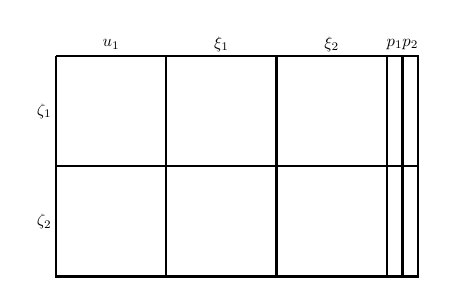
\begin{tikzpicture}[yscale=-1] 

\pgfmathsetmacro{\nt}{7};% time points
\pgfmathsetmacro{\nu}{1}; % controls
\pgfmathsetmacro{\nx}{2}; % states
\pgfmathsetmacro{\np}{2}; % parameters
\pgfmathsetmacro{\nc}{\nu + \nx}; % total continuous

%% control labels
\foreach \k in {1,...,\nu}{
	\pgfmathsetmacro{\x}{0.2*\nt*\k - 0.2/2*(\nt-1)};
	\node () at (\x,-0.05) {\scalebox{0.6}{$u_{\k}$}};
}

%% state labels
\foreach \k in {1,...,\nx}{
	\pgfmathsetmacro{\x}{0.2*\nt*\k + 0.2*\nu*\nt - 0.2/2*(\nt-1)};
	\node () at (\x,-0.05) {\scalebox{0.6}{$\xi_{\k}$}};
}

%% parameter labels
\foreach \k in {1,...,\np}{
	\pgfmathsetmacro{\x}{0.2*\k + 0.2*\nu*\nt + 0.2*\nx*\nt};
	\node () at (\x,-0.05) {\scalebox{0.6}{$p_{\k}$}};
}

%% defects
\foreach \k in {1,...,\nx}{
	\pgfmathsetmacro{\x}{0.2*\nt*\k - 0.2/2*(\nt-1)};
	\node () at (-0.05,\x) {\scalebox{0.6}{$\zeta_{\k}$}};
}


%% controls
\foreach \k in {1,...,\nu}{
	\foreach \j in {1,...,\nx}{
		\foreach \i in {1,...,\nt}{ 
        	\pgfmathsetmacro{\kk}{\k-1};
            \pgfmathsetmacro{\jj}{\j-1};
        	\pgfmathsetmacro{\x}{0.2*\i + 0.2*\kk*\nt};
            \pgfmathsetmacro{\y}{0.2*\i + 0.2*\jj*\nt};
        	\node () at (\x,\y) {\mysparsesymbol};
} 
    \pgfmathsetmacro{\kk}{\k-1};
    \pgfmathsetmacro{\jj}{\j-1};
    \pgfmathsetmacro{\x}{0.2*\kk*\nt + 0.1};
    \pgfmathsetmacro{\y}{0.2*\jj*\nt + 0.1};
	\draw[\mysparseboxcolor,thick](\x,\y) -- (\x+0.2*\nt,\y) -- (\x+0.2*\nt,\y+0.2*\nt) -- (\x,\y+0.2*\nt) -- (\x,\y);
} }

%% states
\foreach \k in {1,...,\nx}{
	\foreach \j in {1,...,\nx}{
		\foreach \i in {1,...,\nt}{ 
        	\pgfmathsetmacro{\kk}{\k-1};
            \pgfmathsetmacro{\jj}{\j-1};
        	\pgfmathsetmacro{\x}{0.2*\i + 0.2*\nu*\nt + 0.2*\kk*\nt};
            \pgfmathsetmacro{\y}{0.2*\i + 0.2*\jj*\nt};
        	\node () at (\x,\y) {\mysparsesymbol};
} 
    \pgfmathsetmacro{\kk}{\k-1};
    \pgfmathsetmacro{\jj}{\j-1};
    \pgfmathsetmacro{\x}{0.2*\kk*\nt + 0.2*\nu*\nt + 0.1};
    \pgfmathsetmacro{\y}{0.2*\jj*\nt + 0.1};
	\draw[\mysparseboxcolor,thick](\x,\y) -- (\x+0.2*\nt,\y) -- (\x+0.2*\nt,\y+0.2*\nt) -- (\x,\y+0.2*\nt) -- (\x,\y);
} }

%% states - full
\foreach \k in {1,...,\nx}{
		\foreach \i in {1,...,\nt}{
        	\foreach \p in {1,...,\nt}{
            
              \pgfmathsetmacro{\kk}{\k-1};
              \pgfmathsetmacro{\x}{0.2*\i + 0.2*\nu*\nt + 0.2*\kk*\nt};
              \pgfmathsetmacro{\y}{0.2*\p + 0.2*\kk*\nt};
            
        	\node () at (\x,\y) {\mysparsesymbol};
} } }

%% parameters
\foreach \k in {1,...,\np}{
	\foreach \j in {1,...,\nx}{
		\foreach \i in {1,...,\nt}{ 
        	\pgfmathsetmacro{\kk}{\k-1};
            \pgfmathsetmacro{\jj}{\j-1};
        	\node () at ( 0.2*\k + 0.2*\nx*\nt + 0.2*\nu*\nt, 0.2*\i + 0.2*\jj*\nt ) {\mysparsesymbol};
} 
    \pgfmathsetmacro{\kk}{\k-1};
    \pgfmathsetmacro{\jj}{\j-1};
    \pgfmathsetmacro{\x}{0.2*\kk + 0.2*\nx*\nt + 0.2*\nu*\nt + 0.1};
    \pgfmathsetmacro{\y}{0.2*\jj*\nt+ 0.1};
	\draw[\mysparseboxcolor,thick](\x,\y) -- (\x+0.2,\y) -- (\x+0.2,\y+0.2*\nt) -- (\x,\y+0.2*\nt) -- (\x,\y);

} }

%% states - full
\foreach \k in {1,...,\nx}{
		\foreach \i in {1,...,\nt}{
        	\foreach \p in {1,...,\nt}{
            
              \pgfmathsetmacro{\kk}{\k-1};
              \pgfmathsetmacro{\x}{0.2*\i + 0.2*\nu*\nt + 0.2*\kk*\nt};
              \pgfmathsetmacro{\y}{0.2*\p + 0.2*\kk*\nt};
            
        	\node () at (\x,\y) {\mytemp};
} } }

\end{tikzpicture}
}
\end{minipage}
\caption{$\bm{D}$ terms.}
% \label{fig:}
\end{subfigure}%
\begin{subfigure}{0.33\textwidth}
\centering
\begin{minipage}{\textwidth}
\tikzsetnextfilename{APS1}

\centering
\resizebox{1\textwidth}{!}{
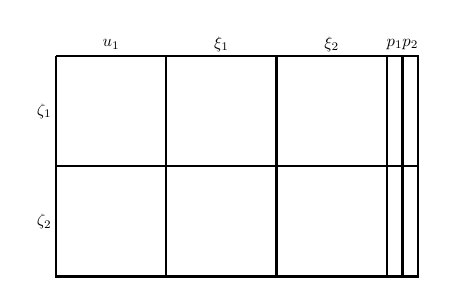
\begin{tikzpicture}[yscale=-1] 

\pgfmathsetmacro{\nt}{7};% time points
\pgfmathsetmacro{\nu}{1}; % controls
\pgfmathsetmacro{\nx}{2}; % states
\pgfmathsetmacro{\np}{2}; % parameters
\pgfmathsetmacro{\nc}{\nu + \nx}; % total continuous

%% control labels
\foreach \k in {1,...,\nu}{
	\pgfmathsetmacro{\x}{0.2*\nt*\k - 0.2/2*(\nt-1)};
	\node () at (\x,-0.05) {\scalebox{0.6}{$u_{\k}$}};
}

%% state labels
\foreach \k in {1,...,\nx}{
	\pgfmathsetmacro{\x}{0.2*\nt*\k + 0.2*\nu*\nt - 0.2/2*(\nt-1)};
	\node () at (\x,-0.05) {\scalebox{0.6}{$\xi_{\k}$}};
}

%% parameter labels
\foreach \k in {1,...,\np}{
	\pgfmathsetmacro{\x}{0.2*\k + 0.2*\nu*\nt + 0.2*\nx*\nt};
	\node () at (\x,-0.05) {\scalebox{0.6}{$p_{\k}$}};
}

%% defects
\foreach \k in {1,...,\nx}{
	\pgfmathsetmacro{\x}{0.2*\nt*\k - 0.2/2*(\nt-1)};
	\node () at (-0.05,\x) {\scalebox{0.6}{$\zeta_{\k}$}};
}


%% controls
\foreach \k in {1,...,\nu}{
	\foreach \j in {1,...,\nx}{
		\foreach \i in {1,...,\nt}{ 
        	\pgfmathsetmacro{\kk}{\k-1};
            \pgfmathsetmacro{\jj}{\j-1};
        	\pgfmathsetmacro{\x}{0.2*\i + 0.2*\kk*\nt};
            \pgfmathsetmacro{\y}{0.2*\i + 0.2*\jj*\nt};
        	\node () at (\x,\y) {\mysparsesymbol};
} 
    \pgfmathsetmacro{\kk}{\k-1};
    \pgfmathsetmacro{\jj}{\j-1};
    \pgfmathsetmacro{\x}{0.2*\kk*\nt + 0.1};
    \pgfmathsetmacro{\y}{0.2*\jj*\nt + 0.1};
	\draw[\mysparseboxcolor,thick](\x,\y) -- (\x+0.2*\nt,\y) -- (\x+0.2*\nt,\y+0.2*\nt) -- (\x,\y+0.2*\nt) -- (\x,\y);
} }

%% states
\foreach \k in {1,...,\nx}{
	\foreach \j in {1,...,\nx}{
		\foreach \i in {1,...,\nt}{ 
        	\pgfmathsetmacro{\kk}{\k-1};
            \pgfmathsetmacro{\jj}{\j-1};
        	\pgfmathsetmacro{\x}{0.2*\i + 0.2*\nu*\nt + 0.2*\kk*\nt};
            \pgfmathsetmacro{\y}{0.2*\i + 0.2*\jj*\nt};
        	\node () at (\x,\y) {\mysparsesymbol};
} 
    \pgfmathsetmacro{\kk}{\k-1};
    \pgfmathsetmacro{\jj}{\j-1};
    \pgfmathsetmacro{\x}{0.2*\kk*\nt + 0.2*\nu*\nt + 0.1};
    \pgfmathsetmacro{\y}{0.2*\jj*\nt + 0.1};
	\draw[\mysparseboxcolor,thick](\x,\y) -- (\x+0.2*\nt,\y) -- (\x+0.2*\nt,\y+0.2*\nt) -- (\x,\y+0.2*\nt) -- (\x,\y);
} }

%% states - full
\foreach \k in {1,...,\nx}{
		\foreach \i in {1,...,\nt}{
        	\foreach \p in {1,...,\nt}{
            
              \pgfmathsetmacro{\kk}{\k-1};
              \pgfmathsetmacro{\x}{0.2*\i + 0.2*\nu*\nt + 0.2*\kk*\nt};
              \pgfmathsetmacro{\y}{0.2*\p + 0.2*\kk*\nt};
            
        	\node () at (\x,\y) {\mysparsesymbol};
} } }

%% parameters
\foreach \k in {1,...,\np}{
	\foreach \j in {1,...,\nx}{
		\foreach \i in {1,...,\nt}{ 
        	\pgfmathsetmacro{\kk}{\k-1};
            \pgfmathsetmacro{\jj}{\j-1};
        	\node () at ( 0.2*\k + 0.2*\nx*\nt + 0.2*\nu*\nt, 0.2*\i + 0.2*\jj*\nt ) {\mysparsesymbol};
} 
    \pgfmathsetmacro{\kk}{\k-1};
    \pgfmathsetmacro{\jj}{\j-1};
    \pgfmathsetmacro{\x}{0.2*\kk + 0.2*\nx*\nt + 0.2*\nu*\nt + 0.1};
    \pgfmathsetmacro{\y}{0.2*\jj*\nt+ 0.1};
	\draw[\mysparseboxcolor,thick](\x,\y) -- (\x+0.2,\y) -- (\x+0.2,\y+0.2*\nt) -- (\x,\y+0.2*\nt) -- (\x,\y);

} }

%% states
\foreach \k in {1,...,\nx}{
	\foreach \j in {1,...,\nx}{
		\foreach \i in {1,...,\nt}{ 
        	\pgfmathsetmacro{\kk}{\k-1};
            \pgfmathsetmacro{\jj}{\j-1};
        	\pgfmathsetmacro{\x}{0.2*\i + 0.2*\nu*\nt + 0.2*\kk*\nt};
            \pgfmathsetmacro{\y}{0.2*\i + 0.2*\jj*\nt};
        	\node () at (\x,\y) {\mytemp};
} } }

\end{tikzpicture}
}
\end{minipage}
\caption{$\bm{A}$ terms.}
% \label{fig:}
\end{subfigure}%
\begin{subfigure}{0.33\textwidth}
\centering
\begin{minipage}{\textwidth}
\input{../ch5/sparsity/APS3}
\end{minipage}
\caption{$\bm{B}$ terms.}
% \label{fig:}
\end{subfigure}%

\begin{subfigure}{0.33\textwidth}
\centering
\begin{minipage}{\textwidth}
\tikzsetnextfilename{APS4}

\centering
\resizebox{1\textwidth}{!}{
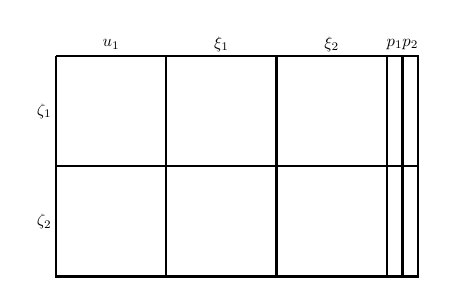
\begin{tikzpicture}[yscale=-1] 

\pgfmathsetmacro{\nt}{7};% time points
\pgfmathsetmacro{\nu}{1}; % controls
\pgfmathsetmacro{\nx}{2}; % states
\pgfmathsetmacro{\np}{2}; % parameters
\pgfmathsetmacro{\nc}{\nu + \nx}; % total continuous

%% control labels
\foreach \k in {1,...,\nu}{
	\pgfmathsetmacro{\x}{0.2*\nt*\k - 0.2/2*(\nt-1)};
	\node () at (\x,-0.05) {\scalebox{0.6}{$u_{\k}$}};
}

%% state labels
\foreach \k in {1,...,\nx}{
	\pgfmathsetmacro{\x}{0.2*\nt*\k + 0.2*\nu*\nt - 0.2/2*(\nt-1)};
	\node () at (\x,-0.05) {\scalebox{0.6}{$\xi_{\k}$}};
}

%% parameter labels
\foreach \k in {1,...,\np}{
	\pgfmathsetmacro{\x}{0.2*\k + 0.2*\nu*\nt + 0.2*\nx*\nt};
	\node () at (\x,-0.05) {\scalebox{0.6}{$p_{\k}$}};
}

%% defects
\foreach \k in {1,...,\nx}{
	\pgfmathsetmacro{\x}{0.2*\nt*\k - 0.2/2*(\nt-1)};
	\node () at (-0.05,\x) {\scalebox{0.6}{$\zeta_{\k}$}};
}


%% controls
\foreach \k in {1,...,\nu}{
	\foreach \j in {1,...,\nx}{
		\foreach \i in {1,...,\nt}{ 
        	\pgfmathsetmacro{\kk}{\k-1};
            \pgfmathsetmacro{\jj}{\j-1};
        	\pgfmathsetmacro{\x}{0.2*\i + 0.2*\kk*\nt};
            \pgfmathsetmacro{\y}{0.2*\i + 0.2*\jj*\nt};
        	\node () at (\x,\y) {\mysparsesymbol};
} 
    \pgfmathsetmacro{\kk}{\k-1};
    \pgfmathsetmacro{\jj}{\j-1};
    \pgfmathsetmacro{\x}{0.2*\kk*\nt + 0.1};
    \pgfmathsetmacro{\y}{0.2*\jj*\nt + 0.1};
	\draw[\mysparseboxcolor,thick](\x,\y) -- (\x+0.2*\nt,\y) -- (\x+0.2*\nt,\y+0.2*\nt) -- (\x,\y+0.2*\nt) -- (\x,\y);
} }

%% states
\foreach \k in {1,...,\nx}{
	\foreach \j in {1,...,\nx}{
		\foreach \i in {1,...,\nt}{ 
        	\pgfmathsetmacro{\kk}{\k-1};
            \pgfmathsetmacro{\jj}{\j-1};
        	\pgfmathsetmacro{\x}{0.2*\i + 0.2*\nu*\nt + 0.2*\kk*\nt};
            \pgfmathsetmacro{\y}{0.2*\i + 0.2*\jj*\nt};
        	\node () at (\x,\y) {\mysparsesymbol};
} 
    \pgfmathsetmacro{\kk}{\k-1};
    \pgfmathsetmacro{\jj}{\j-1};
    \pgfmathsetmacro{\x}{0.2*\kk*\nt + 0.2*\nu*\nt + 0.1};
    \pgfmathsetmacro{\y}{0.2*\jj*\nt + 0.1};
	\draw[\mysparseboxcolor,thick](\x,\y) -- (\x+0.2*\nt,\y) -- (\x+0.2*\nt,\y+0.2*\nt) -- (\x,\y+0.2*\nt) -- (\x,\y);
} }

%% states - full
\foreach \k in {1,...,\nx}{
		\foreach \i in {1,...,\nt}{
        	\foreach \p in {1,...,\nt}{
            
              \pgfmathsetmacro{\kk}{\k-1};
              \pgfmathsetmacro{\x}{0.2*\i + 0.2*\nu*\nt + 0.2*\kk*\nt};
              \pgfmathsetmacro{\y}{0.2*\p + 0.2*\kk*\nt};
            
        	\node () at (\x,\y) {\mysparsesymbol};
} } }

%% parameters
\foreach \k in {1,...,\np}{
	\foreach \j in {1,...,\nx}{
		\foreach \i in {1,...,\nt}{ 
        	\pgfmathsetmacro{\kk}{\k-1};
            \pgfmathsetmacro{\jj}{\j-1};
        	\node () at ( 0.2*\k + 0.2*\nx*\nt + 0.2*\nu*\nt, 0.2*\i + 0.2*\jj*\nt ) {\mysparsesymbol};
} 
    \pgfmathsetmacro{\kk}{\k-1};
    \pgfmathsetmacro{\jj}{\j-1};
    \pgfmathsetmacro{\x}{0.2*\kk + 0.2*\nx*\nt + 0.2*\nu*\nt + 0.1};
    \pgfmathsetmacro{\y}{0.2*\jj*\nt+ 0.1};
	\draw[\mysparseboxcolor,thick](\x,\y) -- (\x+0.2,\y) -- (\x+0.2,\y+0.2*\nt) -- (\x,\y+0.2*\nt) -- (\x,\y);

} }

%% parameters
\foreach \k in {1,...,\np}{
	\foreach \j in {1,...,\nx}{
		\foreach \i in {1,...,\nt}{ 
        	\pgfmathsetmacro{\kk}{\k-1};
            \pgfmathsetmacro{\jj}{\j-1};
        	\node () at ( 0.2*\k + 0.2*\nx*\nt + 0.2*\nu*\nt, 0.2*\i + 0.2*\jj*\nt ) {\mytemp};
} } }

\end{tikzpicture}
}
\end{minipage}
\caption{$\bm{G}$ terms.}
% \label{fig:}
\end{subfigure}%

\caption{Sparsity pattern of $\mathbf{A}_{e1}$ matrix for the defect constraints using a pseudospectral method.}
\label{fig:figsparsityAPS}
\end{figure}


% \begin{figure}[h]

% \centering

% \subfloat[(a) $\bm{D}$ terms.]{
% 	\begin{minipage}{0.33\textwidth}
% 	\tikzsetnextfilename{APS2}

\centering
\resizebox{1\textwidth}{!}{
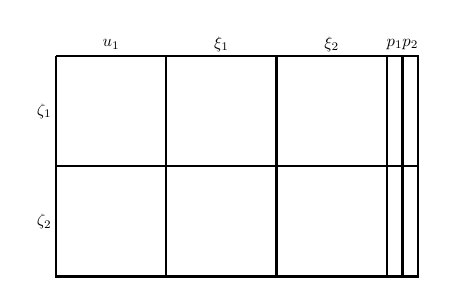
\begin{tikzpicture}[yscale=-1] 

\pgfmathsetmacro{\nt}{7};% time points
\pgfmathsetmacro{\nu}{1}; % controls
\pgfmathsetmacro{\nx}{2}; % states
\pgfmathsetmacro{\np}{2}; % parameters
\pgfmathsetmacro{\nc}{\nu + \nx}; % total continuous

%% control labels
\foreach \k in {1,...,\nu}{
	\pgfmathsetmacro{\x}{0.2*\nt*\k - 0.2/2*(\nt-1)};
	\node () at (\x,-0.05) {\scalebox{0.6}{$u_{\k}$}};
}

%% state labels
\foreach \k in {1,...,\nx}{
	\pgfmathsetmacro{\x}{0.2*\nt*\k + 0.2*\nu*\nt - 0.2/2*(\nt-1)};
	\node () at (\x,-0.05) {\scalebox{0.6}{$\xi_{\k}$}};
}

%% parameter labels
\foreach \k in {1,...,\np}{
	\pgfmathsetmacro{\x}{0.2*\k + 0.2*\nu*\nt + 0.2*\nx*\nt};
	\node () at (\x,-0.05) {\scalebox{0.6}{$p_{\k}$}};
}

%% defects
\foreach \k in {1,...,\nx}{
	\pgfmathsetmacro{\x}{0.2*\nt*\k - 0.2/2*(\nt-1)};
	\node () at (-0.05,\x) {\scalebox{0.6}{$\zeta_{\k}$}};
}


%% controls
\foreach \k in {1,...,\nu}{
	\foreach \j in {1,...,\nx}{
		\foreach \i in {1,...,\nt}{ 
        	\pgfmathsetmacro{\kk}{\k-1};
            \pgfmathsetmacro{\jj}{\j-1};
        	\pgfmathsetmacro{\x}{0.2*\i + 0.2*\kk*\nt};
            \pgfmathsetmacro{\y}{0.2*\i + 0.2*\jj*\nt};
        	\node () at (\x,\y) {\mysparsesymbol};
} 
    \pgfmathsetmacro{\kk}{\k-1};
    \pgfmathsetmacro{\jj}{\j-1};
    \pgfmathsetmacro{\x}{0.2*\kk*\nt + 0.1};
    \pgfmathsetmacro{\y}{0.2*\jj*\nt + 0.1};
	\draw[\mysparseboxcolor,thick](\x,\y) -- (\x+0.2*\nt,\y) -- (\x+0.2*\nt,\y+0.2*\nt) -- (\x,\y+0.2*\nt) -- (\x,\y);
} }

%% states
\foreach \k in {1,...,\nx}{
	\foreach \j in {1,...,\nx}{
		\foreach \i in {1,...,\nt}{ 
        	\pgfmathsetmacro{\kk}{\k-1};
            \pgfmathsetmacro{\jj}{\j-1};
        	\pgfmathsetmacro{\x}{0.2*\i + 0.2*\nu*\nt + 0.2*\kk*\nt};
            \pgfmathsetmacro{\y}{0.2*\i + 0.2*\jj*\nt};
        	\node () at (\x,\y) {\mysparsesymbol};
} 
    \pgfmathsetmacro{\kk}{\k-1};
    \pgfmathsetmacro{\jj}{\j-1};
    \pgfmathsetmacro{\x}{0.2*\kk*\nt + 0.2*\nu*\nt + 0.1};
    \pgfmathsetmacro{\y}{0.2*\jj*\nt + 0.1};
	\draw[\mysparseboxcolor,thick](\x,\y) -- (\x+0.2*\nt,\y) -- (\x+0.2*\nt,\y+0.2*\nt) -- (\x,\y+0.2*\nt) -- (\x,\y);
} }

%% states - full
\foreach \k in {1,...,\nx}{
		\foreach \i in {1,...,\nt}{
        	\foreach \p in {1,...,\nt}{
            
              \pgfmathsetmacro{\kk}{\k-1};
              \pgfmathsetmacro{\x}{0.2*\i + 0.2*\nu*\nt + 0.2*\kk*\nt};
              \pgfmathsetmacro{\y}{0.2*\p + 0.2*\kk*\nt};
            
        	\node () at (\x,\y) {\mysparsesymbol};
} } }

%% parameters
\foreach \k in {1,...,\np}{
	\foreach \j in {1,...,\nx}{
		\foreach \i in {1,...,\nt}{ 
        	\pgfmathsetmacro{\kk}{\k-1};
            \pgfmathsetmacro{\jj}{\j-1};
        	\node () at ( 0.2*\k + 0.2*\nx*\nt + 0.2*\nu*\nt, 0.2*\i + 0.2*\jj*\nt ) {\mysparsesymbol};
} 
    \pgfmathsetmacro{\kk}{\k-1};
    \pgfmathsetmacro{\jj}{\j-1};
    \pgfmathsetmacro{\x}{0.2*\kk + 0.2*\nx*\nt + 0.2*\nu*\nt + 0.1};
    \pgfmathsetmacro{\y}{0.2*\jj*\nt+ 0.1};
	\draw[\mysparseboxcolor,thick](\x,\y) -- (\x+0.2,\y) -- (\x+0.2,\y+0.2*\nt) -- (\x,\y+0.2*\nt) -- (\x,\y);

} }

%% states - full
\foreach \k in {1,...,\nx}{
		\foreach \i in {1,...,\nt}{
        	\foreach \p in {1,...,\nt}{
            
              \pgfmathsetmacro{\kk}{\k-1};
              \pgfmathsetmacro{\x}{0.2*\i + 0.2*\nu*\nt + 0.2*\kk*\nt};
              \pgfmathsetmacro{\y}{0.2*\p + 0.2*\kk*\nt};
            
        	\node () at (\x,\y) {\mytemp};
} } }

\end{tikzpicture}
}
% 	\end{minipage}
% }%
% \subfloat[(b) $\bm{A}$ terms.]{
% 	\begin{minipage}{0.33\textwidth}
% 	\tikzsetnextfilename{APS1}

\centering
\resizebox{1\textwidth}{!}{
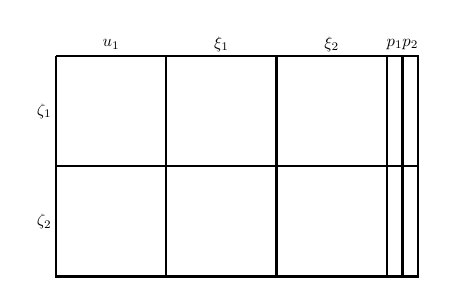
\begin{tikzpicture}[yscale=-1] 

\pgfmathsetmacro{\nt}{7};% time points
\pgfmathsetmacro{\nu}{1}; % controls
\pgfmathsetmacro{\nx}{2}; % states
\pgfmathsetmacro{\np}{2}; % parameters
\pgfmathsetmacro{\nc}{\nu + \nx}; % total continuous

%% control labels
\foreach \k in {1,...,\nu}{
	\pgfmathsetmacro{\x}{0.2*\nt*\k - 0.2/2*(\nt-1)};
	\node () at (\x,-0.05) {\scalebox{0.6}{$u_{\k}$}};
}

%% state labels
\foreach \k in {1,...,\nx}{
	\pgfmathsetmacro{\x}{0.2*\nt*\k + 0.2*\nu*\nt - 0.2/2*(\nt-1)};
	\node () at (\x,-0.05) {\scalebox{0.6}{$\xi_{\k}$}};
}

%% parameter labels
\foreach \k in {1,...,\np}{
	\pgfmathsetmacro{\x}{0.2*\k + 0.2*\nu*\nt + 0.2*\nx*\nt};
	\node () at (\x,-0.05) {\scalebox{0.6}{$p_{\k}$}};
}

%% defects
\foreach \k in {1,...,\nx}{
	\pgfmathsetmacro{\x}{0.2*\nt*\k - 0.2/2*(\nt-1)};
	\node () at (-0.05,\x) {\scalebox{0.6}{$\zeta_{\k}$}};
}


%% controls
\foreach \k in {1,...,\nu}{
	\foreach \j in {1,...,\nx}{
		\foreach \i in {1,...,\nt}{ 
        	\pgfmathsetmacro{\kk}{\k-1};
            \pgfmathsetmacro{\jj}{\j-1};
        	\pgfmathsetmacro{\x}{0.2*\i + 0.2*\kk*\nt};
            \pgfmathsetmacro{\y}{0.2*\i + 0.2*\jj*\nt};
        	\node () at (\x,\y) {\mysparsesymbol};
} 
    \pgfmathsetmacro{\kk}{\k-1};
    \pgfmathsetmacro{\jj}{\j-1};
    \pgfmathsetmacro{\x}{0.2*\kk*\nt + 0.1};
    \pgfmathsetmacro{\y}{0.2*\jj*\nt + 0.1};
	\draw[\mysparseboxcolor,thick](\x,\y) -- (\x+0.2*\nt,\y) -- (\x+0.2*\nt,\y+0.2*\nt) -- (\x,\y+0.2*\nt) -- (\x,\y);
} }

%% states
\foreach \k in {1,...,\nx}{
	\foreach \j in {1,...,\nx}{
		\foreach \i in {1,...,\nt}{ 
        	\pgfmathsetmacro{\kk}{\k-1};
            \pgfmathsetmacro{\jj}{\j-1};
        	\pgfmathsetmacro{\x}{0.2*\i + 0.2*\nu*\nt + 0.2*\kk*\nt};
            \pgfmathsetmacro{\y}{0.2*\i + 0.2*\jj*\nt};
        	\node () at (\x,\y) {\mysparsesymbol};
} 
    \pgfmathsetmacro{\kk}{\k-1};
    \pgfmathsetmacro{\jj}{\j-1};
    \pgfmathsetmacro{\x}{0.2*\kk*\nt + 0.2*\nu*\nt + 0.1};
    \pgfmathsetmacro{\y}{0.2*\jj*\nt + 0.1};
	\draw[\mysparseboxcolor,thick](\x,\y) -- (\x+0.2*\nt,\y) -- (\x+0.2*\nt,\y+0.2*\nt) -- (\x,\y+0.2*\nt) -- (\x,\y);
} }

%% states - full
\foreach \k in {1,...,\nx}{
		\foreach \i in {1,...,\nt}{
        	\foreach \p in {1,...,\nt}{
            
              \pgfmathsetmacro{\kk}{\k-1};
              \pgfmathsetmacro{\x}{0.2*\i + 0.2*\nu*\nt + 0.2*\kk*\nt};
              \pgfmathsetmacro{\y}{0.2*\p + 0.2*\kk*\nt};
            
        	\node () at (\x,\y) {\mysparsesymbol};
} } }

%% parameters
\foreach \k in {1,...,\np}{
	\foreach \j in {1,...,\nx}{
		\foreach \i in {1,...,\nt}{ 
        	\pgfmathsetmacro{\kk}{\k-1};
            \pgfmathsetmacro{\jj}{\j-1};
        	\node () at ( 0.2*\k + 0.2*\nx*\nt + 0.2*\nu*\nt, 0.2*\i + 0.2*\jj*\nt ) {\mysparsesymbol};
} 
    \pgfmathsetmacro{\kk}{\k-1};
    \pgfmathsetmacro{\jj}{\j-1};
    \pgfmathsetmacro{\x}{0.2*\kk + 0.2*\nx*\nt + 0.2*\nu*\nt + 0.1};
    \pgfmathsetmacro{\y}{0.2*\jj*\nt+ 0.1};
	\draw[\mysparseboxcolor,thick](\x,\y) -- (\x+0.2,\y) -- (\x+0.2,\y+0.2*\nt) -- (\x,\y+0.2*\nt) -- (\x,\y);

} }

%% states
\foreach \k in {1,...,\nx}{
	\foreach \j in {1,...,\nx}{
		\foreach \i in {1,...,\nt}{ 
        	\pgfmathsetmacro{\kk}{\k-1};
            \pgfmathsetmacro{\jj}{\j-1};
        	\pgfmathsetmacro{\x}{0.2*\i + 0.2*\nu*\nt + 0.2*\kk*\nt};
            \pgfmathsetmacro{\y}{0.2*\i + 0.2*\jj*\nt};
        	\node () at (\x,\y) {\mytemp};
} } }

\end{tikzpicture}
}
% 	\end{minipage}
% }%
% \subfloat[(c) $\bm{B}$ terms.]{
% 	\begin{minipage}{0.33\textwidth}
% 	\input{../ch5/sparsity/APS3}
% 	\end{minipage}
% }%

% \subfloat[(d) $\bm{G}$ terms.]{
% 	\begin{minipage}{0.33\textwidth}
% 	\tikzsetnextfilename{APS4}

\centering
\resizebox{1\textwidth}{!}{
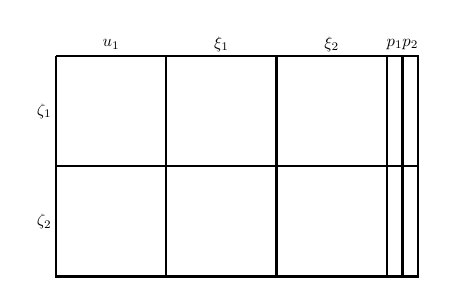
\begin{tikzpicture}[yscale=-1] 

\pgfmathsetmacro{\nt}{7};% time points
\pgfmathsetmacro{\nu}{1}; % controls
\pgfmathsetmacro{\nx}{2}; % states
\pgfmathsetmacro{\np}{2}; % parameters
\pgfmathsetmacro{\nc}{\nu + \nx}; % total continuous

%% control labels
\foreach \k in {1,...,\nu}{
	\pgfmathsetmacro{\x}{0.2*\nt*\k - 0.2/2*(\nt-1)};
	\node () at (\x,-0.05) {\scalebox{0.6}{$u_{\k}$}};
}

%% state labels
\foreach \k in {1,...,\nx}{
	\pgfmathsetmacro{\x}{0.2*\nt*\k + 0.2*\nu*\nt - 0.2/2*(\nt-1)};
	\node () at (\x,-0.05) {\scalebox{0.6}{$\xi_{\k}$}};
}

%% parameter labels
\foreach \k in {1,...,\np}{
	\pgfmathsetmacro{\x}{0.2*\k + 0.2*\nu*\nt + 0.2*\nx*\nt};
	\node () at (\x,-0.05) {\scalebox{0.6}{$p_{\k}$}};
}

%% defects
\foreach \k in {1,...,\nx}{
	\pgfmathsetmacro{\x}{0.2*\nt*\k - 0.2/2*(\nt-1)};
	\node () at (-0.05,\x) {\scalebox{0.6}{$\zeta_{\k}$}};
}


%% controls
\foreach \k in {1,...,\nu}{
	\foreach \j in {1,...,\nx}{
		\foreach \i in {1,...,\nt}{ 
        	\pgfmathsetmacro{\kk}{\k-1};
            \pgfmathsetmacro{\jj}{\j-1};
        	\pgfmathsetmacro{\x}{0.2*\i + 0.2*\kk*\nt};
            \pgfmathsetmacro{\y}{0.2*\i + 0.2*\jj*\nt};
        	\node () at (\x,\y) {\mysparsesymbol};
} 
    \pgfmathsetmacro{\kk}{\k-1};
    \pgfmathsetmacro{\jj}{\j-1};
    \pgfmathsetmacro{\x}{0.2*\kk*\nt + 0.1};
    \pgfmathsetmacro{\y}{0.2*\jj*\nt + 0.1};
	\draw[\mysparseboxcolor,thick](\x,\y) -- (\x+0.2*\nt,\y) -- (\x+0.2*\nt,\y+0.2*\nt) -- (\x,\y+0.2*\nt) -- (\x,\y);
} }

%% states
\foreach \k in {1,...,\nx}{
	\foreach \j in {1,...,\nx}{
		\foreach \i in {1,...,\nt}{ 
        	\pgfmathsetmacro{\kk}{\k-1};
            \pgfmathsetmacro{\jj}{\j-1};
        	\pgfmathsetmacro{\x}{0.2*\i + 0.2*\nu*\nt + 0.2*\kk*\nt};
            \pgfmathsetmacro{\y}{0.2*\i + 0.2*\jj*\nt};
        	\node () at (\x,\y) {\mysparsesymbol};
} 
    \pgfmathsetmacro{\kk}{\k-1};
    \pgfmathsetmacro{\jj}{\j-1};
    \pgfmathsetmacro{\x}{0.2*\kk*\nt + 0.2*\nu*\nt + 0.1};
    \pgfmathsetmacro{\y}{0.2*\jj*\nt + 0.1};
	\draw[\mysparseboxcolor,thick](\x,\y) -- (\x+0.2*\nt,\y) -- (\x+0.2*\nt,\y+0.2*\nt) -- (\x,\y+0.2*\nt) -- (\x,\y);
} }

%% states - full
\foreach \k in {1,...,\nx}{
		\foreach \i in {1,...,\nt}{
        	\foreach \p in {1,...,\nt}{
            
              \pgfmathsetmacro{\kk}{\k-1};
              \pgfmathsetmacro{\x}{0.2*\i + 0.2*\nu*\nt + 0.2*\kk*\nt};
              \pgfmathsetmacro{\y}{0.2*\p + 0.2*\kk*\nt};
            
        	\node () at (\x,\y) {\mysparsesymbol};
} } }

%% parameters
\foreach \k in {1,...,\np}{
	\foreach \j in {1,...,\nx}{
		\foreach \i in {1,...,\nt}{ 
        	\pgfmathsetmacro{\kk}{\k-1};
            \pgfmathsetmacro{\jj}{\j-1};
        	\node () at ( 0.2*\k + 0.2*\nx*\nt + 0.2*\nu*\nt, 0.2*\i + 0.2*\jj*\nt ) {\mysparsesymbol};
} 
    \pgfmathsetmacro{\kk}{\k-1};
    \pgfmathsetmacro{\jj}{\j-1};
    \pgfmathsetmacro{\x}{0.2*\kk + 0.2*\nx*\nt + 0.2*\nu*\nt + 0.1};
    \pgfmathsetmacro{\y}{0.2*\jj*\nt+ 0.1};
	\draw[\mysparseboxcolor,thick](\x,\y) -- (\x+0.2,\y) -- (\x+0.2,\y+0.2*\nt) -- (\x,\y+0.2*\nt) -- (\x,\y);

} }

%% parameters
\foreach \k in {1,...,\np}{
	\foreach \j in {1,...,\nx}{
		\foreach \i in {1,...,\nt}{ 
        	\pgfmathsetmacro{\kk}{\k-1};
            \pgfmathsetmacro{\jj}{\j-1};
        	\node () at ( 0.2*\k + 0.2*\nx*\nt + 0.2*\nu*\nt, 0.2*\i + 0.2*\jj*\nt ) {\mytemp};
} } }

\end{tikzpicture}
}
% 	\end{minipage}
% }%

% \caption{Sparsity pattern of $\mathbf{A}_{e1}$ matrix for the defect constraints using a pseudospectral method.}\label{fig:figsparsityAPS}
% \end{figure}